\documentclass[12pt,a4paper]{report}

% --- packages (BMSCE CSE-DS thesis template; tikz before its libraries) ---
\usepackage{tikz}
\usetikzlibrary{calc}
\usepackage{graphicx}
\usepackage{amsmath}
\usepackage{amssymb}
\usepackage{amsthm}
\usepackage{url}
\usepackage{hyperref}
\usepackage{setspace}
\usepackage{geometry}
\usepackage{titlesec}
\usepackage{tabularx}
\usepackage{etoolbox}
\usepackage{datetime}
\usepackage{lscape}
\usepackage{longtable}
\usetikzlibrary{shapes.geometric, arrows, arrows.meta, positioning, fit, calc, shadows, backgrounds}
\usepackage{float}
\usepackage{listings}
\usepackage{xcolor}
\usepackage{adjustbox}
\usepackage{rotating}
\usepackage{algorithm}
\usepackage{algpseudocode}
\usepackage{algorithmicx}
\usepackage{ragged2e}
\usepackage{afterpage}
\usepackage{multirow}
\usepackage{array}
\usepackage{pgfplots}
\pgfplotsset{compat=1.17}
\usepackage{pgfgantt}

\definecolor{codegray}{rgb}{0.5,0.5,0.5}
\definecolor{codegreen}{rgb}{0,0.6,0}
\definecolor{codeblue}{rgb}{0,0,0.8}
\definecolor{backcolor}{rgb}{0.95,0.95,0.92}

\hypersetup{
    colorlinks=true,
    citecolor=blue,
    linkcolor=blue,
    urlcolor=blue
}

\lstdefinestyle{mystyle}{
    backgroundcolor=\color{backcolor},
    commentstyle=\color{codegreen},
    keywordstyle=\color{codeblue},
    numberstyle=\tiny\color{codegray},
    stringstyle=\color{codegreen},
    basicstyle=\ttfamily\footnotesize,
    breakatwhitespace=false,
    breaklines=true,
    captionpos=b,
    keepspaces=true,
    numbers=left,
    numbersep=5pt,
    showspaces=false,
    showstringspaces=false,
    showtabs=false,
    tabsize=2
}
\lstset{style=mystyle}

\renewcommand{\algorithmicrequire}{\textbf{Input:}}
\renewcommand{\algorithmicensure}{\textbf{Output:}}
\renewcommand{\algorithmiccomment}[1]{\hfill{\small\textit{#1}}}

\geometry{
 a4paper,
 total={170mm,257mm},
 left=20mm,
 top=20mm,
}

% Page border (apply only where needed)
\newcommand{\ApplyBorder}{%
  \begin{tikzpicture}[remember picture,overlay]
    \draw [on background layer,rounded corners=7pt, line width=1.5pt,
           color=black!90, fill=white!20, double distance=1.8pt, double=black!50]
      ($(current page.north west)+(0.4cm,-0.4cm)$)
      rectangle
      ($(current page.south east)+(-0.4cm,0.4cm)$);
  \end{tikzpicture}%
}

\titleformat{\chapter}[display]
  {\normalfont\bfseries}
  {\makebox[\textwidth][l]{\fontsize{36}{42}\selectfont\chaptername\ \thechapter}}
  {0pt}
  {\centering\fontsize{28}{34}\selectfont}
  []
\titlespacing*{\chapter}{0pt}{0pt}{14pt}

\titleformat{\section}
  {\normalfont\fontsize{12}{14}\bfseries}{\thesection}{1em}{}
\titlespacing*{\section}{0pt}{*2}{*1.5}

\titleformat{\subsection}
  {\normalfont\fontsize{12}{14}\bfseries\itshape}{\thesubsection}{1em}{}
\titlespacing*{\subsection}{0pt}{*1.5}{*1}

\titleformat{\subsubsection}
  {\normalfont\fontsize{12}{14}\bfseries\itshape}{\thesubsubsection}{1em}{}
\titlespacing*{\subsubsection}{0pt}{*1}{*0.5}

\setlength{\emergencystretch}{2em}

% Float pages fill from the top with a fixed gap, so two tables on one
% float page sit together instead of being spread over the page height.
\makeatletter
\setlength{\@fptop}{0pt}
\setlength{\@fpsep}{1.5\baselineskip}
\setlength{\@fpbot}{0pt plus 1fil}
\makeatother
\renewcommand{\floatpagefraction}{0.7}

% Table text columns are set ragged-right so narrow cells at body size
% do not stretch inter-word spaces.
\newcolumntype{L}[1]{>{\raggedright\arraybackslash}p{#1}}
\renewcommand{\tabularxcolumn}[1]{>{\raggedright\arraybackslash}p{#1}}
\newdateformat{mydateformat}{\twodigit{\THEDAY}-\twodigit{\THEMONTH}-\THEYEAR}

\usepackage{fancyhdr}
\setlength{\headheight}{15pt}
\fancypagestyle{plain}{%
  \fancyhf{}
  \renewcommand{\headrulewidth}{0pt}
  \renewcommand{\footrulewidth}{0pt}
}
\fancypagestyle{romanstyle}{%
  \fancyhf{}
  \fancyfoot[C]{\roman{page}}
  \renewcommand{\headrulewidth}{0pt}
  \renewcommand{\footrulewidth}{0pt}
}
\fancypagestyle{chapterstyle}{
  \fancyhf{}
  \fancyhead[L]{\textbf{VisionFood QAI: AI-Powered Quality Inspection}}
  \fancyfoot[L]{\small Dept. of CSE (Data Science), BMSCE}
  \fancyfoot[C]{\small 2026--27}
  \fancyfoot[R]{\thepage}
  \renewcommand{\headrulewidth}{1.8pt}
  \renewcommand{\footrulewidth}{1.8pt}
}

\newtheorem{theorem}{Theorem}
\newtheorem{lemma}[theorem]{Lemma}
\newtheorem{corollary}[theorem]{Corollary}
\theoremstyle{definition}
\newtheorem{definition}{Definition}
\theoremstyle{remark}
\newtheorem{remark}{Remark}

% Notation shortcuts
\newcommand{\Rfill}{R_{\mathrm{fill}}}
\newcommand{\mAP}{\mathrm{mAP}}

% Diagram styles shared by all chapters
\tikzset{
  blk/.style={draw, rounded corners=2pt, align=center, font=\footnotesize, minimum height=8mm, fill=white},
  stage/.style={blk, fill=blue!6},
  data/.style={blk, fill=gray!10},
  dec/.style={blk, fill=orange!12},
  res/.style={blk, fill=green!10},
  arr/.style={-{Stealth[length=2mm]}, semithick},
  grp/.style={draw, dashed, rounded corners=4pt, inner sep=6pt}
}

\renewcommand{\bibname}{References}

\begin{document}
\linespread{1.39}\selectfont
\pagestyle{plain}

%======================================================================
\begin{titlepage}
\ApplyBorder
    \begin{center}
        \textsc{\Large \textbf{\textcolor{blue}{B.M.S. COLLEGE OF ENGINEERING}}}\\[0.2cm]
        \textsc{\large \textbf{(Autonomous College under VTU)}}\\[0.2cm]
        \textsc{\large \textbf{Bull Temple Road, Basavangudi, Bangalore - 560019}}\\[0.5cm]

        
\includegraphics[scale=0.6]{logo.png}\\[0.2cm]
        \textit{a Thesis on}\\[0.2cm]
        \textsc{\textbf{\textcolor{red}{VisionFood QAI: AI-Powered Quality Inspection for Food and Beverage Manufacturing}}}\\[0.1cm]
        \textit{(Project Work -- Phase 2)}\\[0.2cm]
        \textit{in fulfillment of the requirements for the award of degree}\\[0.2cm]

        \textbf{BACHELOR OF ENGINEERING}\\[0.15cm]
        \textit{in}\\[0.2cm]
        \textbf{Computer Science \& Engineering (Data Science)}\\[0.2cm]

        \textit{ by}\\[0.2cm]
        \textbf{Shreyas Bairy K S (1BM23CD058)}\\[0.2cm]
        \textbf{Sushanth S (1BM23CD063)}\\[0.2cm]
        \textbf{Ullas N (1BM23CD067)}\\[0.5cm]

        \textbf{Under the Guidance of}\\[0.25cm]
        \textbf{Prof. Nayana N Kumar}\\[0.15cm]
        Project Guide\\[0.4cm]
        \textbf{Department of CSE (Data Science)}, \\
        \textbf{B.M.S. College of Engineering}\\[0.3cm]

        \textbf{AY 2026-2027}
    \end{center}
\end{titlepage}

%======================================================================
\newpage
\pagenumbering{roman}
\pagestyle{romanstyle}
\ApplyBorder
\addcontentsline{toc}{chapter}{Certificate}
\begin{center}
    \textsc{\Large \textbf{\textcolor{blue}{B.M.S. COLLEGE OF ENGINEERING}}}\\[0.1cm]
    \textsc{\large \textbf{(Autonomous College under VTU)}}\\[0.1cm]
    \textsc{\large \textbf{Bull Temple Road, Basavangudi, Bangalore - 560019}}\\[0.4cm]

    
\includegraphics[scale=0.4]{logo.png}\\[0.1cm]
    \textbf{Department of Computer Science and Engineering} \textbf{(Data Science)}\\[0.1cm]
    \textbf{\Large \underline{CERTIFICATE}}\\[0.1cm]
\end{center}

\noindent
This is to certify that the project entitled ``\textbf{VisionFood QAI: AI-Powered Quality Inspection for Food and Beverage Manufacturing}'' is a bona fide work carried out by the following students for the course Project Work -- Phase 2 (Course Code: \textbf{23DS7PWPP2}). It is certified that all corrections and suggestions indicated during the internal assessments have been incorporated in the final thesis submitted to the departmental library. The project thesis has been approved as it meets the academic requirements prescribed for the Bachelor of Engineering Degree in respect of project work.

\begin{center}
    \textbf{\underline{Candidate details}}
\end{center}

\begin{center}
\begin{tabularx}{\textwidth}{|c|X|c|}
    \hline
    \textbf{SL. NO.} & \textbf{Student Name} & \textbf{USN} \\
    \hline
    1 & Shreyas Bairy K S & 1BM23CD058 \\
    \hline
    2 & Sushanth S & 1BM23CD063 \\
    \hline
    3 & Ullas N & 1BM23CD067 \\
    \hline
\end{tabularx}
\end{center}

\vspace{1cm}

\begin{center}
\begin{tabular*}{\textwidth}{@{\extracolsep{\fill}} l c r}
\textbf{Prof. Nayana N Kumar} & \textbf{Dr. Shambhavi B R} & \textbf{Dr. Bheemsha Arya} \\
Project Guide & Professor \& HOD & Principal \\
\end{tabular*}
\end{center}\vspace{0.2cm}

\noindent
\begin{center}
    \textbf{Examiners}\\[0.1cm]
\end{center}
    \textbf{Name of Examiner} \hfill \textbf{Signature of the examiner} \\[0.1cm]
    \textbf{1.} \hfill \rule{5cm}{0.4pt} \\[0.1cm]
    \textbf{2.} \hfill \rule{5cm}{0.4pt} \\

\vfill
\onehalfspacing

%======================================================================
\newpage
\ApplyBorder
\addcontentsline{toc}{chapter}{Declaration}
\begin{center}
        \textsc{\Large \textbf{\textcolor{blue}{B.M.S. COLLEGE OF ENGINEERING}}}\\[0.2cm]
        \textsc{\large \textbf{(Autonomous College under VTU)}}\\[0.2cm]
        \textsc{\large \textbf{Bull Temple Road, Basavangudi, Bangalore - 560019}}\\[0.5cm]
        
\includegraphics[width=0.2\textwidth]{logo.png}\\[0.2cm]
\end{center}

\begin{center}
    \textbf{\Large \underline{DECLARATION}}
\end{center}

\noindent We hereby declare that the project thesis entitled \textbf{\textit{``VisionFood QAI: AI-Powered Quality Inspection for Food and Beverage Manufacturing''}} is a bona fide work carried out by us under the guidance of \textbf{Prof. Nayana N Kumar}, Department of Computer Science and Engineering (Data Science), B.M.S. College of Engineering, Bengaluru, in partial fulfillment of the requirements of the degree of Bachelor of Engineering in Computer Science \& Engineering (Data Science) of Visvesvaraya Technological University, Belagavi.
We further declare that, to the best of our knowledge and belief, this thesis has not been submitted either in part or in full to any other university or college.
\vspace{0.3cm}

\begin{center}
    \textbf{\underline{Candidate details}}
\end{center}

\begin{center}
\begin{tabularx}{\textwidth}{|c|X|c|c|}
    \hline
    \textbf{SL. NO.} & \textbf{Student Name} & \textbf{USN} & \textbf{Student's Signature} \\
    \hline
    1 & Shreyas Bairy K S & 1BM23CD058 & \\
    \hline
    2 & Sushanth S & 1BM23CD063 & \\
    \hline
    3 & Ullas N & 1BM23CD067 & \\
    \hline
\end{tabularx}
\end{center}

\vspace{1.2cm}
\begin{flushleft}
    Date: \rule{4cm}{0.4pt} \hfill Place: Bengaluru
\end{flushleft}

%======================================================================
\newpage
\pagestyle{romanstyle}
\ApplyBorder
\addcontentsline{toc}{chapter}{Acknowledgments}
\begin{center}
\textbf{\Large Acknowledgments}
\end{center}

\noindent The satisfaction that accompanies the completion of the second phase of this \textit{\textbf{Capstone Project}} would be incomplete without acknowledging the people whose guidance and encouragement made it possible.\\
\noindent We express our heartfelt gratitude to \textbf{Dr. B. S. Ragini Narayan}, \textit{Chairperson}, Donor Trustee, Member Secretary \& Chairperson, BMSET; \textbf{Dr. P. Dayananda Pai}, \textit{Member Life Trustee}, BMSET; and \textbf{Dr. Bheemsha Arya}, \textit{Principal}, B.M.S. College of Engineering, for providing the infrastructure required to complete this project.\\
\noindent We are grateful to \textbf{Dr. Shambhavi B R}, Head of the Department, Computer Science and Engineering (Data Science), and to the project coordinators for their constant support.\\
\noindent We express our sincere thanks to our guide, \textbf{Prof. Nayana N Kumar}, Department of Computer Science and Engineering (Data Science), for her guidance, timely reviews, and encouragement throughout both phases of the project.\\
\noindent We also thank all faculty members of the Department of Computer Science and Engineering (Data Science) for their views and suggestions.

\vspace{1.8cm}
\begin{flushright}
Shreyas Bairy K S (1BM23CD058)\\
Sushanth S (1BM23CD063)\\
Ullas N (1BM23CD067)\\
\end{flushright}

%======================================================================
\newpage
% border on every page of the contents and lists, however many pages they take
\AddToHook{shipout/background}[frontborder]{\put(0,0){\ApplyBorder}}
\tableofcontents
\begin{center}
    \addcontentsline{toc}{chapter}{\textbf{List of Tables}}
    \listoftables
\end{center}
\begin{center}
    \addcontentsline{toc}{chapter}{List of Figures}
    \listoffigures
\end{center}

\clearpage
\RemoveFromHook{shipout/background}[frontborder]
\chapter*{\centering List of Abbreviations}
\addcontentsline{toc}{chapter}{List of Abbreviations}
\begin{center}
\begin{tabularx}{\textwidth}{|l|X|}
\hline
\textbf{Abbreviation} & \textbf{Expansion} \\ \hline
AP / mAP & Average Precision / mean Average Precision \\ \hline
API & Application Programming Interface \\ \hline
C2PSA & Cross-stage partial block with Position-Sensitive Attention (YOLO11) \\ \hline
C3k2 & Cross-stage partial bottleneck with kernel-2 option (YOLO11) \\ \hline
DFL & Distribution Focal Loss \\ \hline
FAR / FRR & False Accept Rate / False Reject Rate \\ \hline
FP16 / FP32 & 16-bit / 32-bit floating point \\ \hline
GFLOPs & Giga floating-point operations \\ \hline
IoU & Intersection over Union \\ \hline
KD & Knowledge Distillation \\ \hline
KPI & Key Performance Indicator \\ \hline
MCC & Matthews Correlation Coefficient \\ \hline
NMS & Non-Maximum Suppression \\ \hline
ONNX & Open Neural Network Exchange \\ \hline
ORT & ONNX Runtime \\ \hline
PET & Polyethylene terephthalate (bottle material) \\ \hline
REST & Representational State Transfer \\ \hline
ROI & Region of Interest \\ \hline
RTSP & Real-Time Streaming Protocol \\ \hline
SAHI & Slicing Aided Hyper Inference \\ \hline
SDG & Sustainable Development Goal \\ \hline
SPPF & Spatial Pyramid Pooling -- Fast \\ \hline
TRT & NVIDIA TensorRT \\ \hline
VRAM & Video Random-Access Memory (GPU memory) \\ \hline
WAL & Write-Ahead Log (SQLite journal mode) \\ \hline
\end{tabularx}
\end{center}

%======================================================================
\newpage
\pagenumbering{arabic}
\setcounter{page}{1}
\chapter*{\centering Abstract}
\addcontentsline{toc}{chapter}{Abstract}
\noindent Packaged food and beverage lines still depend heavily on human inspectors, who cannot keep pace with several products per second and who tire over a shift. The first phase of this project proposed a broad inspection architecture; this second phase narrowed it to inspection stations that were built, measured, and deployed. The work had six objectives: a bottle-cap defect detector with threshold analysis, an audited dataset with a defined evaluation protocol, a geometric fill-level estimator with configurable limits, accelerated inference engines, a label-defect prototype for an industrial cosmetic tube, and an operator dashboard with an audit trail. For cap inspection, the Phase 1 pipeline of a bottle detector followed by a MobileNetV3-Small classifier, which reached 86.5\% accuracy, was replaced by a single YOLO11m instance-segmentation student distilled from a YOLO11x-seg teacher through normalised feature alignment at three backbone and attention modules. The student labels six cap states on three synchronised camera views, and an asymmetric quality gate converts its detections into pass, reject, review, or failed-inspection verdicts. The fill-level station combines a bottle detector, a liquid-surface detector, and a closed-form fill ratio with a review band around the underfill and overfill limits. The label prototype localises four printed regions on 1504 by 8000 pixel tube scans by template matching and scores each region with an EfficientAD anomaly model trained only on good labels. All models were exported through ONNX to TensorRT FP16 engines and served by a FastAPI backend and React dashboard in Docker, with every inspection written to SQLite. On the held-out test split of 354 images, the student matched the teacher's mask mAP at IoU 0.5 of 0.995 with 2.8 times fewer parameters and exceeded its strict-IoU mask mAP (0.927 against 0.912); the FP16 engine scored 0.928. Replaying the quality gate produced no false accepts among 153 defective caps and no false rejects among 201 good caps. The liquid-surface detector reached AP of 0.923 at IoU 0.5, the median fill-ratio error from surface localisation was 0.002, and 34 of 35 fill verdicts agreed with the annotated surface. TensorRT reduced the three-view network time from 21.0 ms to 7.4 ms; the closed loop with synchronous audit storage ran at a median of 299 ms per bottle, so storage, not inference, limits throughput. In the label prototype, template matching located all four regions on all 120 scans, and grayscale anomaly models caught 91 to 94 percent of defective crops, although one region still raised too many false alarms. The project shows that a distilled segmentation model, a transparent geometric rule, and an auditable deployment can deliver measurable inspection quality, and it contributes to SDG 9 and SDG 12 by making automated inspection affordable for small and mid-size producers.

\vspace{1em}
\noindent\textbf{Keywords:} bottle-cap inspection; knowledge distillation; YOLO11 instance segmentation; fill-level estimation; anomaly detection; TensorRT; quality gate; operator dashboard.

%======================================================================
\newpage
\pagestyle{chapterstyle}

%======================================================================
\chapter{Introduction}
\label{ch:intro}

This chapter places the second phase of VisionFood QAI in context. It summarises what Phase 1 delivered, explains why the scope was narrowed and the architecture changed, states the Phase 2 objectives in measurable form, and defines the problem the remaining chapters address.

\section{Background}
\label{sec:background}

Visual inspection is the last line of defence between a filling or labelling machine and the consumer. On a beverage line the two most frequent visual rejects concern the closure and the fill level: a cap that is missing, open, misplaced, or damaged breaks the seal, and a container filled below or above its band misstates the declared volume and wastes product. On cosmetic and personal-care lines the printed label carries the brand, the ingredient list, the batch and expiry codes, and the barcode, so a torn, smudged, or partly missing print is a regulatory as well as a cosmetic defect.

Manual inspection does not scale to these lines. A filler running at 300 bottles per minute presents a new container every 200 ms, and inspectors examining reflective plastic or glossy print lose consistency over a shift~\cite{banus2021}. Rule-based machine vision, built from edge detection and pattern matching, works for a fixed product but must be re-tuned whenever a bottle shape, cap colour, or label layout changes~\cite{farhangi2024}. Deep convolutional networks learn the visual patterns directly from data and have reached high accuracy on food-packaging defects~\cite{banus2021,liu2025}, yet published systems rarely report what matters to a plant: the rate at which defective products are passed, the rate at which good products are discarded, and the end-to-end latency of the deployed system~\cite{liakos2025}.

\noindent\textbf{Outcome of Phase 1.} Phase 1 surveyed eighteen studies, proposed a product-profile-driven architecture with a YOLOv8 detector, an EfficientViT-M5 confirmation classifier, Monte Carlo Dropout uncertainty, and a REMEDY routing engine, and built a first bottle prototype. The prototype detected bottles and caps with a YOLO detector (precision 0.869, recall 0.973, mAP@0.5 of 0.958, mAP@0.5:0.95 of 0.786 on a three-class cap set), classified the cap crop with MobileNetV3-Small, and computed fill ratio from a water-surface detector. The cap classifier reached 86.5\% accuracy (precision and recall 0.870), and the dashboard reported 466--678\,ms per uploaded image on a development machine.

The Phase 1 conference submission (CSITSS 2026, Paper 1204) was reviewed in August 2026. The reviewers asked for evaluation on an untouched test split, product-level false-accept and false-reject rates, measured latency, a justification of the cap classifier's accuracy, and a scope that matched what had actually been tested. These comments, together with the Phase 1 evaluation feedback, shaped Phase 2.

\noindent\textbf{Direction of Phase 2.}Phase 2 therefore moved from a broad architecture to a set of inspection stations that are built, measured, and deployed:
\begin{itemize}
    \item \textbf{Station 1 (cap)} replaces the detector-plus-classifier cascade with one distilled instance-segmentation network that labels six cap states on three camera views.
    \item \textbf{Station 2 (fill level)} formalises the geometric fill-ratio rule, adds a review band, and measures its error.
    \item \textbf{Label prototype} extends inspection to printed labels on an industrial cosmetic tube supplied as the Himalaya NSC dataset.
    \item \textbf{Deployment} compiles every model to a TensorRT engine and serves the stations through a containerised backend, an operator dashboard, and an SQLite audit trail.
\end{itemize}
Product formats, the REMEDY engine, Monte Carlo Dropout, and SKU profiles from the Phase 1 design were not carried forward; Section~\ref{sec:scope} lists what is in and out of scope.

\section{Objectives}
\label{sec:objectives}

\noindent\textbf{Primary objective.} Develop and evaluate a bottle-cap defect detector with small-object-aware localisation and threshold analysis, deployable at line rate on a single workstation GPU.

\noindent\textbf{Specific objectives.}
\begin{enumerate}
    \item[\textbf{O1.}] Preserve and audit the cap dataset and all model artefacts (PyTorch, ONNX, TensorRT): document per-split and per-class counts, capture resolution, and object-size distribution; verify that the deployed FP16 engine preserves the accuracy of the trained model; and identify a capture-session-grouped held-out test as the benchmark for future model versions.
    \item[\textbf{O2.}] Build a fill-level estimator from a bottle detector and a liquid-surface detector with a closed-form fill ratio and configurable underfill and overfill limits, and measure its ratio error and verdict agreement on held-out images (target: verdict agreement $\geq 0.93$).
    \item[\textbf{O3.}] Optimise inference by exporting every model to a TensorRT FP16 engine, and measure per-stage and closed-loop latency against PyTorch and ONNX Runtime baselines (targets: network time $<100$\,ms for three views; closed-loop cycle $\leq 200$\,ms for 300 bottles per minute).
    \item[\textbf{O4.}] Prototype a label-defect detector for the Himalaya NSC tube label: template-matching localisation of four printed regions, ROI cropping, and per-region anomaly models, with honestly reported limitations.
    \item[\textbf{O5.}] Deliver an operator dashboard with live KPIs, a review queue for uncertain products, replay of stored inspections, and an exportable SQLite audit trail, packaged with Docker.
\end{enumerate}

The quantitative targets for the cap station were carried over from Phase 1: image-level accuracy $\geq 0.93$, precision $\geq 0.93$, recall $\geq 0.97$, false-accept rate $\leq 3\%$, and false-reject rate $\leq 7\%$. All targets are compared with measured outcomes in Table~\ref{tab:targets}, including the ones that were missed.

\section{Problem Statement}
\label{sec:problem-statement}

The core problem is to decide, for every product on a moving line, whether its closure, fill level, and printed label are acceptable, with error rates and latency that a plant can verify and audit. Four difficulties make this hard.

First, the decisive evidence is small. A droplet on a wet cap, a dent on a damaged cap, the thread gap of an open cap, or a smudge on a few square millimetres of print occupies a small fraction of the region an inspector looks at. A model must keep that fine detail through its down-sampling layers.

Second, the two error types are not equally costly. Passing a defective product exposes the consumer and the brand; rejecting a good product costs material. A useful system must make the asymmetry explicit, send doubtful cases to a human, and report both error rates rather than a single accuracy figure.

Third, accuracy and speed compete. Large networks extract finer features but are too slow for a 200\,ms cycle on one GPU, and a model that is fast in isolation can still miss the line rate once image transfer, post-processing, and storage are added.

Fourth, defects are scarce. Defective labels in particular are rare and varied, so a supervised classifier for each defect type cannot be trained from the few examples available.

\noindent\textbf{Scope.}\label{sec:scope}In scope are transparent PET bottles (cap and fill-level stations) and the Himalaya Winter Defense Moisturizing Cream 50\,ml tube label (prototype). Out of scope are other package types, chemical or microbial contamination, label checks on bottles, remediation routing, and claims about physical fill volume, because no volumetric ground truth was available.

\section{Summary}
\label{sec:intro-summary}

Phase 2 turns the Phase 1 proposal into measured stations. A distilled YOLO11m segmentation model inspects caps behind an asymmetric quality gate, a geometric rule estimates fill level, an anomaly-detection prototype inspects printed labels, and all of them run as optimised engines behind an auditable dashboard. Chapter~\ref{ch:lit} reviews the literature on food and beverage inspection, real-time segmentation, knowledge distillation, anomaly detection, and inference optimisation. Chapter~\ref{ch:method} specifies the requirements and presents the proposed method, the system architecture, the datasets, and the experimental setup. Chapter~\ref{ch:planning} gives the work breakdown, critical path, schedule, responsibilities, risks, and resources. Chapter~\ref{ch:impl} gives the algorithms, loss functions, and integration details. Chapter~\ref{ch:results} reports and discusses the results against every target, and Chapter~\ref{ch:concl} concludes with learnings, the complex-engineering-problem justification, future work, and the SDG alignment.

%======================================================================
\chapter{Literature Review}
\label{ch:lit}

This chapter reviews the work that the Phase 2 design builds on. Phase 1 surveyed food-quality inspection broadly; this review keeps the studies that bear directly on the stations that were built and adds the literature the Phase 2 decisions depend on: instance segmentation, knowledge distillation, reduced-precision inference, class-imbalance handling, and unsupervised anomaly detection for printed surfaces. Each theme ends with what it implies for this project.

\section{Visual Inspection in Food and Beverage Packaging}
\label{sec:lit-food}

\textit{Classical machine vision.} Farhangi \textit{et al.}~\cite{farhangi2024} inspected caps, liquid level, and label placement on liquid bottles with a CMOS camera, edge detection, and pattern matching, reporting 95.6\% average accuracy. The method works because the product, lighting, and camera pose are fixed; every new bottle or cap design requires new rules.

\textit{CNN classification.} Ban\'us \textit{et al.}~\cite{banus2021} compared ResNet, VGG, and DenseNet backbones for thermoformed food packages and validated the best model on a production line with very low false-accept and false-reject rates. Their study is one of few that report both error types, and it shows that imaging design and dataset curation matter as much as the network. Subramanian \textit{et al.}~\cite{subramanian2025} used an optimised ResNet-50 for manufacturing defects. Chatchapol \textit{et al.}~\cite{chatchapol2024} classified beverage fill level and lid sealing with a CNN on an embedded GPU, reaching 98.89\% liquid-level accuracy, but they classify the whole image and do not localise the liquid surface, so the result cannot be expressed as a fill ratio.

\textit{Detection.} Liu \textit{et al.}~\cite{liu2025} added CBAM attention and adaptive feature fusion to YOLOv5 for five food-packaging defects (7,400 images, accuracy 0.96, recall 0.94). Nguyen \textit{et al.}~\cite{nguyen2025} integrated YOLOv8 with a PLC and multi-threaded acquisition and reported above 90\% accuracy across defect types. Kavitha \textit{et al.}~\cite{kavitha2024} coupled YOLO detection to Arduino-driven sorting. These systems localise defects, but they report validation accuracy rather than product-level error rates, and only Nguyen \textit{et al.} measure the latency of the full loop.

\textit{Surveys and data-centric work.} Liakos \textit{et al.}~\cite{liakos2025} reviewed machine learning for food quality control and found beverages to be a small minority of studied applications; they list data scarcity and integration with legacy systems as open problems. Xiong \textit{et al.}~\cite{xiong2024} showed in a food-packaging case study that improving data quality can matter as much as changing the model. Sensor-heavy approaches~\cite{krishnan2024,cao2025,du2025} monitor quality along the supply chain but do not inspect visual defects on the line.

\begin{table}[htbp]
\centering
\caption{Comparison of representative packaging-inspection studies}
\label{tab:lit-compare}
\footnotesize
\begin{tabularx}{\textwidth}{|p{2.6cm}|p{2.4cm}|p{2.6cm}|p{2.4cm}|X|}
\hline
\textbf{Study} & \textbf{Task} & \textbf{Method} & \textbf{Reported result} & \textbf{Gap relative to this project} \\ \hline
Farhangi \textit{et al.}~\cite{farhangi2024} & Cap, level, label on bottles & Edge detection, pattern matching & 95.6\% accuracy & Hand-tuned rules per product \\ \hline
Ban\'us \textit{et al.}~\cite{banus2021} & Thermoformed food packs & DenseNet, ResNet, VGG & Very low FAR/FRR on line & Classification only; no localisation \\ \hline
Chatchapol \textit{et al.}~\cite{chatchapol2024} & Fill level, lid seal & CNN, embedded GPU & 98.89\% level accuracy & No surface localisation, no ratio \\ \hline
Liu \textit{et al.}~\cite{liu2025} & Five packaging defects & YOLOv5 + CBAM + ASFF & Acc.\ 0.96, recall 0.94 & No product-level error rates or latency \\ \hline
Nguyen \textit{et al.}~\cite{nguyen2025} & Industrial surfaces & YOLOv8 + PLC & $>$90\% accuracy & Not food-specific \\ \hline
Truong and Luong~\cite{truong2024} & Reusable food packaging & Autoencoder anomaly detection & Detects cracks and contamination & Threshold sensitivity, false alarms \\ \hline
Ribeiro \textit{et al.}~\cite{ribeiro2025} & Pharmaceutical bottles & Multi-view, incremental learning & Adapts to new defects & Pharmaceutical domain \\ \hline
\end{tabularx}
\end{table}

\noindent\textit{Implication.} The literature supports learned localisation, but it rarely reports false-accept and false-reject rates, threshold margins, or deployed latency. Phase 2 reports all three for every station.

\section{Real-Time Detection and Instance Segmentation}
\label{sec:lit-seg}

One-stage detectors in the YOLO family predict boxes and classes in a single forward pass~\cite{redmon2016}. Ultralytics YOLOv8~\cite{jocher2023} and YOLO11~\cite{jocher2024} are anchor-free and decouple the classification and box-regression heads; box regression uses a distribution focal loss (DFL) over discretised offsets. Their segmentation variants follow YOLACT~\cite{bolya2019}: the network predicts a small set of full-image mask prototypes and, for every detected instance, a vector of coefficients; the instance mask is the sigmoid of the coefficient-weighted sum of prototypes, cropped to the box. This keeps mask prediction nearly as cheap as detection, unlike two-stage Mask R-CNN~\cite{he2017maskrcnn}, which pools a feature map for each proposal.

YOLO11 introduces three blocks that matter for this project. The C3k2 block is a cross-stage partial bottleneck that carries edge and texture features through the backbone. The SPPF block pools the deepest backbone map at several receptive fields in sequence, giving multi-scale context at little cost. The C2PSA block adds position-sensitive self-attention to the deepest features, so the network can weigh where in the image the evidence lies. Section~\ref{sec:kd-impl} distils features at exactly these three blocks.

\noindent\textit{Implication.} A segmentation detector returns class, box, and mask in one pass. The mask gives the quality gate and the audit record the cap's exact region, which a whole-image classifier cannot provide.

\section{Knowledge Distillation}
\label{sec:lit-kd}

Knowledge distillation trains a compact \textit{student} to imitate a larger \textit{teacher}. Hinton \textit{et al.}~\cite{hinton2015} matched temperature-softened class probabilities (\textit{response} or \textit{logit} distillation), so that the student learns the teacher's similarity structure between classes. FitNets~\cite{romero2015} introduced \textit{hint} learning: a learned regressor maps an intermediate student layer onto a teacher layer and the two are matched with an $L_2$ loss. Zagoruyko and Komodakis~\cite{zagoruyko2017} transferred spatial attention maps instead of raw activations.

Distilling detectors is harder than distilling classifiers, because most image locations are background and dominate any loss summed over the feature map. Chen \textit{et al.}~\cite{chen2017kd} combined hint, logit, and bounded regression terms for two-stage detectors. Wang \textit{et al.}~\cite{wang2019fgfi} imitated features only near object anchors, and showed that full-map imitation can hurt because background swamps the signal. Normalising features before matching, or restricting the loss to informative regions, are the two common remedies.

\noindent\textit{Implication.} For bottle caps, the decisive evidence is fine-grained (droplets, dents, a thread gap), so matching only the teacher's outputs would tell the student \emph{what} to predict but not \emph{where} to look. Phase 2 uses feature-level distillation at the three YOLO11 blocks above, with channel-wise $L_2$ normalisation to keep the background from dominating (Section~\ref{sec:kd-impl}).

\section{Reduced-Precision and Accelerated Inference}
\label{sec:lit-trt}

Mixed-precision arithmetic stores weights and activations in 16-bit floating point while keeping numerically sensitive operations in 32 bits~\cite{micikevicius2018}. Integer quantisation goes further, replacing floating-point arithmetic with 8-bit integers~\cite{jacob2018}; both can change accuracy as well as speed, so each must be measured on the target hardware. NVIDIA TensorRT~\cite{tensorrt} compiles a network graph for a specific GPU: it fuses layers, selects kernels by timing them, and supports FP16 and INT8 precision with static or dynamic input shapes. The ONNX format and ONNX Runtime~\cite{onnxruntime} provide a vendor-neutral intermediate representation and a portable CPU/GPU runtime.

\noindent\textit{Implication.} A TensorRT engine is tied to the GPU and library version that built it. The deployment therefore compiles engines on the target machine, caches them under a version tag, and falls back to ONNX Runtime and then PyTorch when no compatible GPU is present (Section~\ref{sec:deploy-impl}).

\section{Class Imbalance and Evaluation}
\label{sec:lit-imb}

Defect data are usually imbalanced because compliant products far outnumber defective ones. Standard remedies are re-weighting or re-sampling the training data~\cite{buda2018}, class-balanced losses based on the effective number of samples~\cite{cui2019}, and focal loss, which down-weights easy examples~\cite{lin2017focal}. Mixup~\cite{zhang2018mixup} and CutMix~\cite{yun2019} regularise training but can blend away a defect that covers a small part of the object. The benefit of any remedy is best judged with class-sensitive metrics: per-class precision and recall, Cohen's $\kappa$~\cite{cohen1960}, and the Matthews correlation coefficient~\cite{chicco2020}. When an error count is zero, an exact binomial (Clopper--Pearson) bound~\cite{clopper1934} states how large the true rate could still be.

\noindent\textit{Implication.} Phase 2 reports per-class AP, $\kappa$, MCC, and exact confidence bounds on false-accept and false-reject rates instead of a single accuracy figure.

\section{Anomaly Detection for Printed Labels}
\label{sec:lit-anom}

Supervised detectors need labelled examples of every defect type. For printed labels, defects are rare and open-ended, so unsupervised anomaly detection, which learns only from good samples, is the usual alternative. The MVTec AD benchmark~\cite{bergmann2019} established the task of image- and pixel-level anomaly detection on industrial objects and textures. PatchCore~\cite{roth2022} stores a coreset of pretrained patch features from good images and scores a test patch by its distance to the nearest stored feature; it is among the most accurate methods, but its memory bank grows with the training set and nearest-neighbour search slows inference. EfficientAD~\cite{batzner2024} trains a lightweight student network to reproduce a pretrained teacher's features on good images, and an autoencoder to model global layout; disagreement between student and teacher, and between student and autoencoder, produces a pixel-level anomaly map at millisecond-level latency. The Anomalib library~\cite{akcay2022} provides reference implementations of both.

Localising the regions to inspect is a separate problem. Template matching by normalised cross-correlation~\cite{lewis1995,brunelli2009} finds a known pattern in an image without training data and is reliable when the pattern's appearance and scale are stable. Learned detectors are more flexible, but very large images must either be down-scaled, which destroys small structures, or sliced into tiles as in SAHI~\cite{akyon2022}. Generative models such as StyleGAN2-ADA~\cite{karras2020} can synthesise additional good samples when training data are limited.

\noindent\textit{Implication.} For a fixed label layout scanned at high resolution, template matching gives deterministic localisation without labelled boxes, and EfficientAD gives per-region anomaly maps from good samples only. Phase 2 tested both PatchCore and a YOLO-plus-SAHI localiser before settling on this combination (Section~\ref{sec:risk}).

\section{Limitations of Existing Systems}
\label{sec:limitations}

Table~\ref{tab:limitations} summarises the gaps that the Phase 2 objectives address.

\begin{table}[htbp]
\centering
\caption{Limitations of existing systems and the Phase 2 response}
\label{tab:limitations}
\footnotesize
\begin{tabularx}{\textwidth}{|p{3.6cm}|X|p{1.4cm}|}
\hline
\textbf{Limitation} & \textbf{Evidence and Phase 2 response} & \textbf{Obj.} \\ \hline
Validation-only accuracy & Most packaging studies report validation accuracy~\cite{liu2025,nguyen2025}. Phase 2 reports held-out test results for FP32 and deployed FP16 models and product-level FAR/FRR with exact bounds. & Primary, O1 \\ \hline
No threshold analysis & Decision thresholds are rarely justified. Phase 2 sweeps the gate thresholds and reports the margin to the nearest error. & Primary \\ \hline
Whole-image fill classification & Fill level is classified, not measured~\cite{chatchapol2024}. Phase 2 localises the meniscus, computes a ratio, and derives its sensitivity to pixel error. & O2 \\ \hline
Heavy models at the edge & Accurate backbones are slow~\cite{subramanian2025}. Phase 2 distils a 62\,M-parameter teacher into a 22\,M student and compiles FP16 engines. & Primary, O3 \\ \hline
Scarce defect labels & Rare, varied defects~\cite{liakos2025,truong2024}. The label prototype trains on good samples only. & O4 \\ \hline
No auditable deployment & Few systems store evidence per product. Phase 2 stores raw frames, labels, and verdicts in SQLite and exposes them in a dashboard. & O5 \\ \hline
\end{tabularx}
\end{table}

These gaps lead to the architecture in Chapter~\ref{ch:method}: distilled segmentation for caps, geometric measurement for fill level, good-only anomaly detection for labels, and an optimised, auditable deployment around all three.

%======================================================================
\chapter{Methodology}
\label{ch:method}

This chapter specifies what the system must do, describes the proposed method and the system at the level of modules and data flow, and defines the datasets, experimental setup, metrics, baselines, and resources used. Algorithms, equations of the models, and pseudocode are deferred to Chapter~\ref{ch:impl}; the project plan is given in Chapter~\ref{ch:planning}.

\section{Requirements Specification}
\label{sec:req-spec}

The requirements follow from the objectives in Section~\ref{sec:objectives} and from the conference reviews of Phase 1. Table~\ref{tab:fr} lists the functional requirements and Table~\ref{tab:nfr} the non-functional requirements with their quantitative targets. Every target is checked against a measured value in Table~\ref{tab:targets}.

\begin{table}[htbp]
\centering
\caption{Functional requirements}
\label{tab:fr}
\begin{tabularx}{\textwidth}{|L{1.2cm}|X|L{1.6cm}|}
\hline
\textbf{ID} & \textbf{Requirement} & \textbf{Obj.} \\ \hline
FR1 & Label the cap of every bottle from three synchronised views as one of six states and return \texttt{PASS}, \texttt{REJECT}, \texttt{UNCERTAIN}, or \texttt{INSPECTION\_FAILED}. & Primary \\ \hline
FR2 & Measure the fill ratio of a bottle from one side view and judge it against configurable underfill and overfill limits. & O2 \\ \hline
FR3 & Locate the four printed regions of the tube label, score each with its own anomaly model, and fail the label if any region fails or is missing. & O4 \\ \hline
FR4 & Store the raw frames, YOLO-format labels, verdict, and decision reason of every inspection. & O1, O5 \\ \hline
FR5 & Show live KPIs, a review queue for uncertain products, replay of stored inspections, CSV export, and run-time threshold settings in a dashboard. & O5 \\ \hline
FR6 & Switch between stations so that only one station's engines occupy GPU memory at a time. & O3, O5 \\ \hline
\end{tabularx}
\end{table}

\begin{table}[htbp]
\centering
\caption{Non-functional requirements and targets}
\label{tab:nfr}
\begin{tabularx}{\textwidth}{|L{1.2cm}|L{3.0cm}|X|}
\hline
\textbf{ID} & \textbf{Quality} & \textbf{Target} \\ \hline
NFR1 & Cap accuracy & Image-level accuracy $\geq0.93$, precision $\geq0.93$, recall $\geq0.97$ on a held-out test split. \\ \hline
NFR2 & Fail-safe decisions & False-accept rate $\leq3\%$, false-reject rate $\leq7\%$; a doubtful product is never passed automatically. \\ \hline
NFR3 & Fill accuracy & Fill-state agreement with the annotated surface $\geq0.93$. \\ \hline
NFR4 & Latency & Network time $<100$\,ms for three views; closed-loop cycle $\leq200$\,ms (300 bottles per minute). \\ \hline
NFR5 & Portability & Same code natively and in Docker; fall back to ONNX Runtime and then PyTorch when no compatible GPU is present. \\ \hline
NFR6 & Auditability & Every verdict traceable to stored evidence; engines versioned; paths set by configuration. \\ \hline
\end{tabularx}
\end{table}

\section{Proposed Methodology}
\label{sec:proposed-method}

The method replaces the broad Phase 1 design with three stations, each built around one inspection question, one set of models, and one decision rule. Three principles guided the design.
\begin{enumerate}
    \item \textbf{One station, one question.} Each station answers one inspection question (cap state, fill level, or label integrity) with its own models, decision rule, audit database, and API namespace. Stations share a server and a dashboard only for convenience, so one can be changed or removed without touching the others.
    \item \textbf{Asymmetric, fail-safe decisions.} A doubtful product is never passed automatically. Every station has four outcomes: \texttt{PASS}, \texttt{REJECT}, \texttt{UNCERTAIN} (sent to human review without ejection), and \texttt{INSPECTION\_FAILED} (the input could not be evaluated).
    \item \textbf{Evidence before verdict.} Every verdict is stored with the raw frames, the model outputs, and the reason for the decision, so any automated decision can be audited and the stored images can be re-used for training.
\end{enumerate}

\subsection{Station 1: cap inspection}
The three camera views of one bottle are resized to the network input and passed through the cap network as one batch of three. Non-maximum suppression (NMS) is applied to each view separately. The network is a YOLO11m instance-segmentation \emph{student} that was trained with feature-level distillation from a frozen YOLO11x-seg \emph{teacher} (Section~\ref{sec:kd-impl}); the teacher and the distillation projectors exist only during training. Each view is judged on its own, and the bottle verdict is \emph{defect-dominant}: a defect seen by any camera rejects the bottle. This design replaces the Phase 1 cascade of a bottle/cap detector followed by a MobileNetV3-Small crop classifier; the reasons are given in Section~\ref{sec:why-seg}.

\subsection{Station 2: fill level}
Figure~\ref{fig:fill-pipeline} shows the fill station as a multi-stage pipeline. Stage 1 localises the bottle with a YOLOv8s detector and keeps the highest-scoring bottle box. Stage 2 detects the liquid surface (meniscus) with a separate YOLOv8n detector run on the full frame, associates a surface box with the bottle, trims the bottle box to remove detector padding, and computes the fill ratio $\Rfill$ in closed form. Stage 3 maps the ratio into one of three fill classes (underfill, acceptable, overfill) and then into a gate verdict, with a review band around each limit when the meniscus detection is weak. The limits are configuration values, not learned parameters.

\begin{figure}[htbp]
\centering
\begin{adjustbox}{max width=\textwidth}
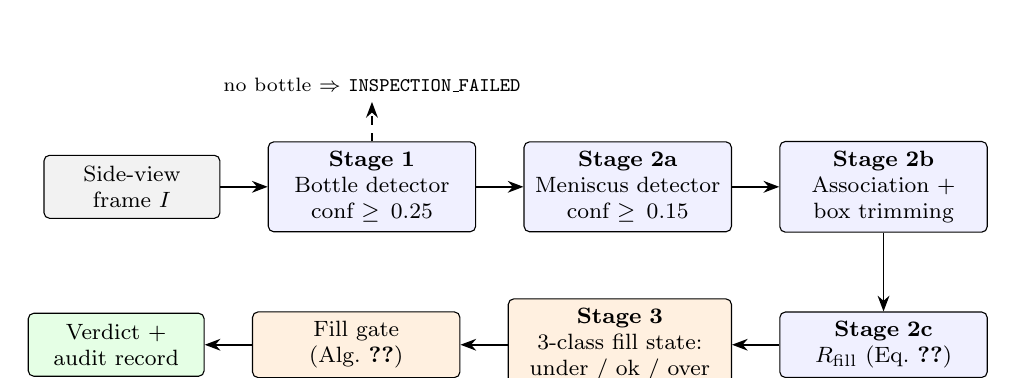
\begin{tikzpicture}[node distance=5mm, every node/.style={font=\footnotesize}]
\node[data, text width=2.0cm] (in) {Side-view\\frame $I$};
\node[stage, text width=2.4cm, right=6mm of in] (s1) {\textbf{Stage 1}\\Bottle detector\\conf $\geq 0.25$};
\node[stage, text width=2.4cm, right=6mm of s1] (s2a) {\textbf{Stage 2a}\\Meniscus detector\\conf $\geq 0.15$};
\node[stage, text width=2.4cm, right=6mm of s2a] (s2b) {\textbf{Stage 2b}\\Association +\\box trimming};
\node[stage, text width=2.4cm, below=10mm of s2b] (s2c) {\textbf{Stage 2c}\\$R_{\mathrm{fill}}$ (Eq.~\ref{eq:rfill})};
\node[dec, text width=2.6cm, left=6mm of s2c] (s3) {\textbf{Stage 3}\\3-class fill state:\\under / ok / over};
\node[dec, text width=2.4cm, left=6mm of s3] (g) {Fill gate\\(Alg.~\ref{alg:fillgate})};
\node[res, text width=2.0cm, left=6mm of g] (v) {Verdict +\\audit record};
\foreach \a/\b in {in/s1,s1/s2a,s2a/s2b,s2b/s2c,s2c/s3,s3/g,g/v} \draw[arr] (\a) -- (\b);
\draw[arr, dashed] (s1.north) -- ++(0,5mm) node[above, font=\scriptsize, align=center]{no bottle $\Rightarrow$ \texttt{INSPECTION\_FAILED}};
\end{tikzpicture}
\end{adjustbox}
\caption[Multi-stage fill-level pipeline (Station 2)]{Multi-stage fill-level pipeline (Station 2). Stage 1 localises the bottle, Stage 2 localises the meniscus and measures the ratio, and Stage 3 classifies the fill state and applies the review band.}
\label{fig:fill-pipeline}
\end{figure}

\subsection{Label prototype (O4)}
The label prototype inspects the printed label of the Himalaya Winter Defense Moisturizing Cream (50\,ml) tube. The input is a flat, unwrapped scan of about $1504{\times}8000$ pixels. Because the label wraps around a cylinder, each printed region appears twice in the scan. Figure~\ref{fig:label-pipeline} shows the three steps: (i) \emph{preprocessing and localisation}, in which the scan is converted to grayscale and four full-region templates are located by coarse-to-fine normalised cross-correlation, keeping the complete (uncut) occurrence of each region; (ii) \emph{ROI cropping}, in which each located region is cut out and rotated upright; and (iii) \emph{model routing}, in which each crop is sent to the anomaly model trained for that region. A label fails if any region scores above its calibrated threshold or if any region cannot be located.

\begin{figure}[htbp]
\centering
\begin{adjustbox}{max width=\textwidth}
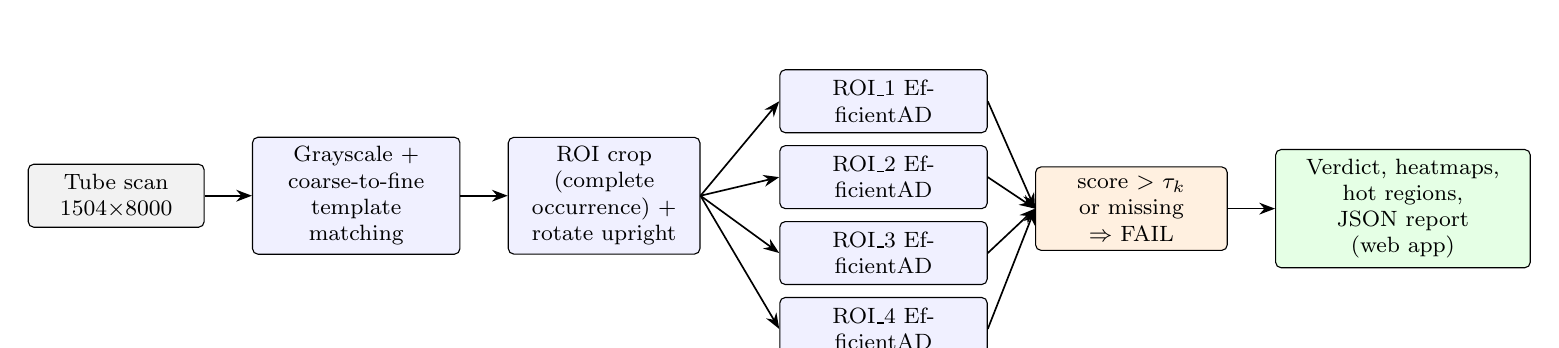
\begin{tikzpicture}[node distance=5mm, every node/.style={font=\footnotesize}]
\node[data, text width=2.0cm] (scan) {Tube scan\\$1504{\times}8000$};
\node[stage, text width=2.4cm, right=6mm of scan] (pre) {Grayscale +\\coarse-to-fine\\template matching};
\node[stage, text width=2.2cm, right=6mm of pre] (crop) {ROI crop\\(complete\\occurrence) +\\rotate upright};
\node[stage, text width=2.4cm, right=10mm of crop, yshift=12mm] (r1) {ROI\_1 EfficientAD};
\node[stage, text width=2.4cm, below=1.5mm of r1] (r2) {ROI\_2 EfficientAD};
\node[stage, text width=2.4cm, below=1.5mm of r2] (r3) {ROI\_3 EfficientAD};
\node[stage, text width=2.4cm, below=1.5mm of r3] (r4) {ROI\_4 EfficientAD};
\node[dec, text width=2.2cm, right=6mm of r2, yshift=-4mm] (agg) {score $>$ $\tau_k$\\or missing\\$\Rightarrow$ FAIL};
\draw[arr] (scan) -- (pre); \draw[arr] (pre) -- (crop);
\foreach \r in {r1,r2,r3,r4} {\draw[arr] (crop.east) -- (\r.west); \draw[arr] (\r.east) -- (agg.west);}
\node[res, text width=3.0cm, right=6mm of agg] (exp) {Verdict, heatmaps, hot regions,\\JSON report (web app)};
\draw[arr] (agg) -- (exp);
\end{tikzpicture}
\end{adjustbox}
\caption[Label-defect prototype pipeline]{Label-defect prototype: template-matching localisation, ROI cropping, and routing of each crop to its own anomaly model.}
\label{fig:label-pipeline}
\end{figure}

The four regions are: ROI\_1, the logo and product name; ROI\_2, the ingredient line and paragraph; ROI\_3, the address, regulatory numbers, manufacturing and expiry dates, and barcode; and ROI\_4, the ``3 Way Care'' graphic.

\section{System Architecture}
\label{sec:system-architecture}

Figure~\ref{fig:system-architecture} shows the complete system. The input layer acquires frames: three synchronised views per bottle for the cap station, one side view for the fill station, and a full unwrapped scan for the label prototype. The inference layer runs each station's models as TensorRT engines (cap and fill) or ONNX models (label). The decision layer turns model outputs into verdicts with station-specific rules. The persistence and presentation layer writes each result to SQLite and to disk, pushes it to the dashboard over a WebSocket, and drives the reject actuator.

\begin{figure}[htbp]
\centering
\begin{adjustbox}{max width=\textwidth}
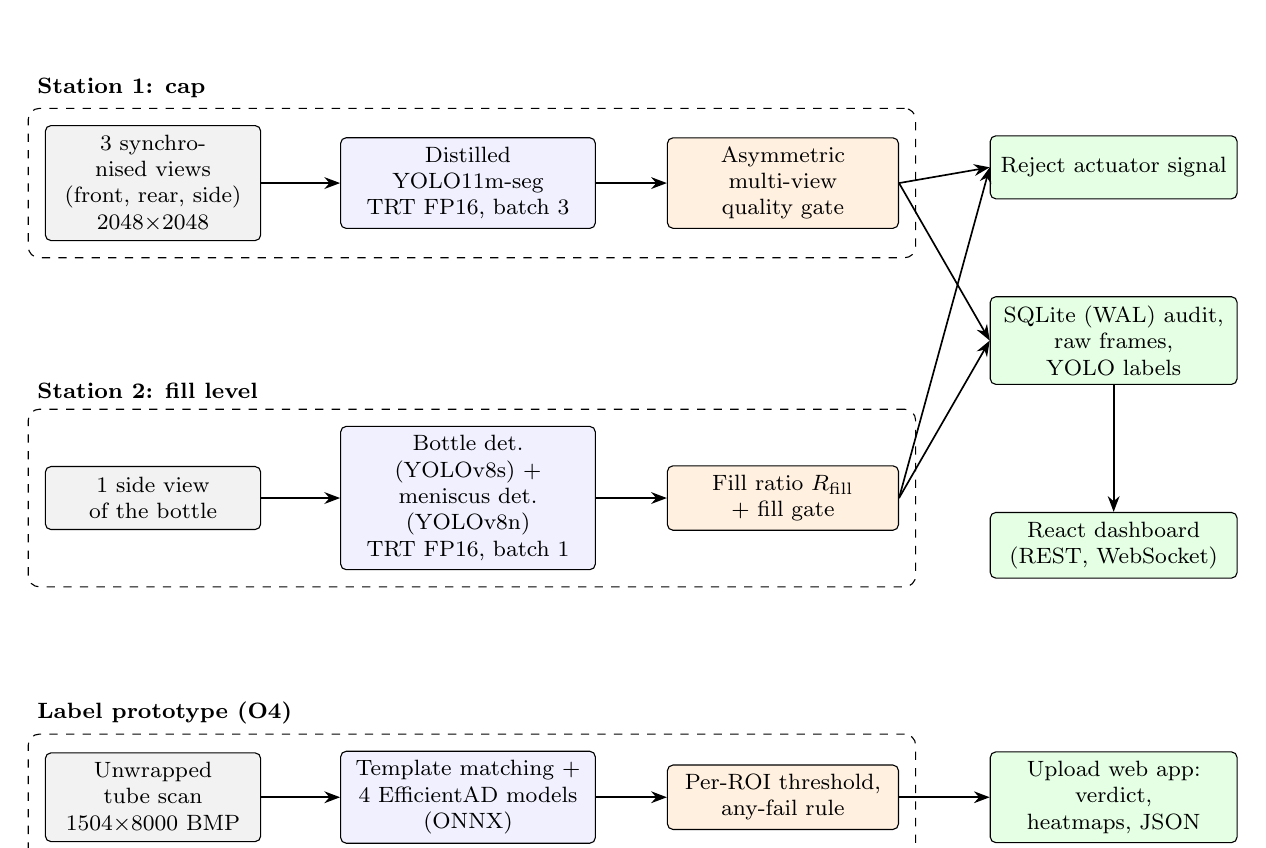
\begin{tikzpicture}[every node/.style={font=\footnotesize}]
% rows far enough apart that each group's heading clears the box above it
\def\rA{0} \def\rB{-4.0} \def\rC{-7.8}
% inputs
\node[data, text width=2.5cm] (c1) at (0,\rA) {3 synchronised views\\(front, rear, side)\\$2048{\times}2048$};
\node[data, text width=2.5cm] (c2) at (0,\rB) {1 side view\\of the bottle};
\node[data, text width=2.5cm] (c3) at (0,\rC) {Unwrapped tube scan\\$1504{\times}8000$ BMP};
% models
\node[stage, text width=3.0cm] (m1) at (4.0,\rA) {Distilled YOLO11m-seg\\TRT FP16, batch 3};
\node[stage, text width=3.0cm] (m2) at (4.0,\rB) {Bottle det.\ (YOLOv8s) +\\meniscus det.\ (YOLOv8n)\\TRT FP16, batch 1};
\node[stage, text width=3.0cm] (m3) at (4.0,\rC) {Template matching +\\4 EfficientAD models\\(ONNX)};
% decisions
\node[dec, text width=2.7cm] (d1) at (8.0,\rA) {Asymmetric multi-view\\quality gate};
\node[dec, text width=2.7cm] (d2) at (8.0,\rB) {Fill ratio $R_{\mathrm{fill}}$\\+ fill gate};
\node[dec, text width=2.7cm] (d3) at (8.0,\rC) {Per-ROI threshold,\\any-fail rule};
% outputs
\node[res, text width=2.9cm] (act) at (12.2,0.2) {Reject actuator signal};
\node[res, text width=2.9cm] (db) at (12.2,-2.0) {SQLite (WAL) audit,\\raw frames, YOLO labels};
\node[res, text width=2.9cm] (ui) at (12.2,-4.6) {React dashboard\\(REST, WebSocket)};
\node[res, text width=2.9cm] (web) at (12.2,\rC) {Upload web app:\\verdict, heatmaps, JSON};
\foreach \a/\b in {c1/m1,c2/m2,c3/m3,m1/d1,m2/d2,m3/d3,db/ui,d3/web} \draw[arr] (\a) -- (\b);
\draw[arr] (d1.east) -- (act.west);
\draw[arr] (d1.east) -- (db.west);
\draw[arr] (d2.east) -- (db.west);
\draw[arr] (d2.east) -- (act.west);
\begin{scope}[on background layer]
\node[grp, fit=(c1)(m1)(d1), label={[font=\footnotesize\bfseries, anchor=south west]north west:Station 1: cap}] {};
\node[grp, fit=(c2)(m2)(d2), label={[font=\footnotesize\bfseries, anchor=south west]north west:Station 2: fill level}] {};
\node[grp, fit=(c3)(m3)(d3), label={[font=\footnotesize\bfseries, anchor=south west]north west:Label prototype (O4)}] {};
\end{scope}
\end{tikzpicture}
\end{adjustbox}
\caption[Overall VisionFood QAI architecture]{Overall VisionFood QAI architecture. Each row is an independent station with its own models and decision rule; the cap and fill stations share the audit and dashboard layer, and the label prototype runs as a separate upload-and-inspect application. Blue: inference; orange: decision; green: outputs.}
\label{fig:system-architecture}
\end{figure}

Figure~\ref{fig:deploy} shows how the cap and fill stations are served. A FastAPI application exposes Station 1 under \texttt{/api/*} and Station 2 under \texttt{/api/fill/*}, with one WebSocket stream per station. Each station is owned by a service object that holds the engine, the gate, the audit logger, and the overlay renderer. Only one station's engines occupy GPU memory at a time: the cap engine is loaded at start-up, the fill engines are loaded on demand, and a station switch in the dashboard unloads one set before loading the other. The backend and an nginx container serving the built dashboard are started together with Docker Compose; the same backend can also run natively and serve the built dashboard itself.

\begin{figure}[htbp]
\centering
\begin{adjustbox}{max width=\textwidth}
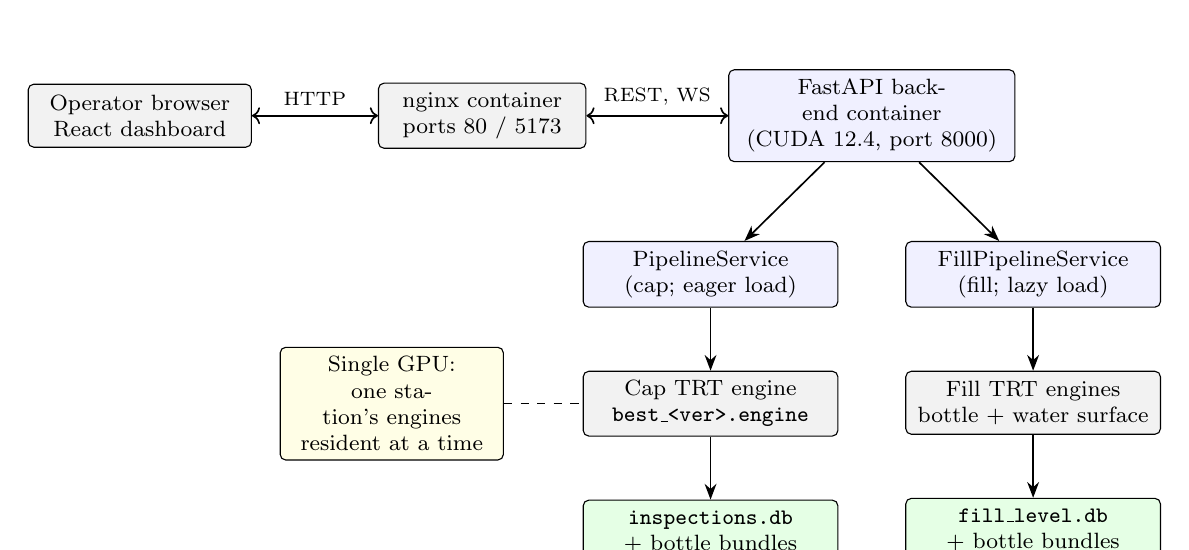
\begin{tikzpicture}[node distance=5mm, every node/.style={font=\footnotesize}]
\node[blk, fill=gray!10, text width=2.6cm] (br) {Operator browser\\React dashboard};
\node[blk, fill=gray!10, text width=2.4cm, right=16mm of br] (ng) {nginx container\\ports 80 / 5173};
\node[stage, text width=3.4cm, right=18mm of ng] (api) {FastAPI backend container\\(CUDA 12.4, port 8000)};
\node[stage, text width=3.0cm, below left=10mm and -14mm of api] (s1) {PipelineService\\(cap; eager load)};
\node[stage, text width=3.0cm, below right=10mm and -14mm of api] (s2) {FillPipelineService\\(fill; lazy load)};
\node[data, text width=3.0cm, below=8mm of s1] (e1) {Cap TRT engine\\\texttt{best\_<ver>.engine}};
\node[data, text width=3.0cm, below=8mm of s2] (e2) {Fill TRT engines\\bottle + water surface};
\node[res, text width=3.0cm, below=8mm of e1] (d1) {\texttt{inspections.db}\\+ bottle bundles};
\node[res, text width=3.0cm, below=8mm of e2] (d2) {\texttt{fill\_level.db}\\+ bottle bundles};
\node[blk, fill=yellow!10, text width=2.6cm, left=10mm of e1] (gpu) {Single GPU:\\one station's engines\\resident at a time};
\draw[arr, <->] (br) -- node[above, font=\scriptsize]{HTTP} (ng);
\draw[arr, <->] (ng) -- node[above, font=\scriptsize]{REST, WS} (api);
\draw[arr] (api) -- (s1); \draw[arr] (api) -- (s2);
\draw[arr] (s1) -- (e1); \draw[arr] (s2) -- (e2);
\draw[arr] (e1) -- (d1); \draw[arr] (e2) -- (d2);
\draw[dashed] (gpu) -- (e1);
\end{tikzpicture}
\end{adjustbox}
\caption[Deployment architecture]{Deployment architecture. Two Docker containers (dashboard and backend) share bind-mounted model and audit folders with the host. Station switching unloads one engine set before loading the other.}
\label{fig:deploy}
\end{figure}

\section{Dataset}
\label{sec:dataset}
\label{sec:data-sources}

Table~\ref{tab:datasets} lists every dataset used; Appendix~\ref{appendix:dataset} describes their collection, composition, annotation format, limitations, and availability in detail. The cap set is public and was used as exported, with its own training, validation, and test splits. The fill-level detectors were trained on merged public sets. The label scans were supplied by an industrial partner. The code and data are kept in the following locations:
\begin{itemize}
    \item Repository: \url{https://github.com/ShreyasBairyKS/Capstone-Project} (cap and fill stations, dashboard, deployment).
    \item Label prototype branch: \url{https://github.com/ShreyasBairyKS/Capstone-Project/tree/himalaya-label-detection}.
    \item \sloppy Local project folder \texttt{E:\textbackslash P-25 Vision Food ai}, which holds the NSC scans in \texttt{dataset\textbackslash NSC} and the label-prototype working tree in \texttt{himalaya\_\allowbreak label\_\allowbreak detection}.
\end{itemize}
The NSC scans are not redistributed because the product images belong to the manufacturer.

\begin{table}[htbp]
\centering
\caption{Datasets used in Phase 2}
\label{tab:datasets}
\begin{tabularx}{\textwidth}{|L{2.9cm}|L{2.7cm}|X|L{2.4cm}|}
\hline
\textbf{Dataset} & \textbf{Used for} & \textbf{Content and split} & \textbf{Licence / source} \\ \hline
\texttt{bottle\_cap\_\allowbreak sdp} v7~\cite{roboflowcap} & Station 1 teacher and student & 6 cap classes, polygon masks; 7,458 / 712 / 354 images (train / valid / test), $2048{\times}2048$ & Roboflow Universe, CC BY 4.0 \\ \hline
Merged bottle/cap sets & Station 2 bottle detector & 4 public sources; 2,286 / 417 / 280 images; 2,133 / 774 / 356 bottle boxes & Public, CC BY 4.0 \\ \hline
\texttt{fill-level} v1~\cite{fillds1} + \texttt{bottle-\allowbreak liquid-\allowbreak level} v2~\cite{fillds2} & Station 2 meniscus detector & Single class \texttt{water\_\allowbreak surface}; 545 / 31 / 41 images; 1,683 / 54 / 76 boxes & Roboflow Universe, CC BY 4.0 \\ \hline
Four-class cap classification set & Model-selection benchmark (Table~\ref{tab:classifiers}) & 7,540 images; 308-image test split & Earlier project data \\ \hline
Himalaya NSC & Label prototype (O4) & 120 unwrapped tube scans, $\approx1504{\times}8000$ BMP: 78 good, 42 defective & Industrial partner (local copy) \\ \hline
\end{tabularx}
\end{table}

\section{Experimental Setup and Evaluation Metrics}
\label{sec:setup}

\subsection{Experimental Configuration}
\label{sec:exp-config}
Training ran on an NVIDIA RTX A5000 (24\,GB). All latency figures were measured inside the production Docker image on one workstation (RTX A5000, Intel Xeon W-2295 with 36 threads, CUDA 12.1 PyTorch build 2.4.1, TensorRT 10.16.1, Ultralytics 8.4.192, ONNX Runtime 1.31.1 with the CPU provider). Each GPU configuration was warmed up with 5 calls and timed over 100 calls; medians are reported. Station 1 accuracy is reported for both the trained FP32 checkpoint and the deployed FP16 engine. The cap models were selected on the 712-image validation split and reported on the 354-image test split, which was used neither for training nor for model selection or threshold setting. The closed-loop stress test drives the complete Station 1 path for 500 unpaced cycles and a second run of 300 cycles paced at 150 bottles per minute. Label-prototype results come from the experiments on the \texttt{himalaya-label-detection} branch and are reported with the protocol under which each number was obtained.

\subsection{Evaluation Metrics}
\label{sec:metrics}
With $TP$, $FP$, $FN$, and $TN$ the counts of true positives, false positives, false negatives, and true negatives,
\begin{equation}
    P=\frac{TP}{TP+FP},\qquad R=\frac{TP}{TP+FN},\qquad F_1=\frac{2PR}{P+R}.
    \label{eq:prf}
\end{equation}
\noindent\textbf{Detection and segmentation.} A detection is a true positive when its intersection over union (IoU) with an unmatched ground-truth instance of the same class reaches a threshold $t$. The average precision $\mathrm{AP}_t$ is the area under the precision--recall curve at IoU $t$; $\mAP@0.5$ averages it over classes at $t=0.5$, and $\mAP@0.5{:}0.95$ also averages over $t\in\{0.50,0.55,\dots,0.95\}$, which rewards tight boxes and masks. Mask AP uses mask IoU; box AP uses box IoU.

\noindent\textbf{Product-level errors.} For the cap gate a defective cap is the positive class. The false-accept rate (defect passed) and false-reject rate (good product rejected) are
\begin{equation}
    \mathrm{FAR}=\frac{\#\{\text{defective}\rightarrow\texttt{PASS}\}}{\#\text{defective}},\qquad
    \mathrm{FRR}=\frac{\#\{\text{good}\rightarrow\texttt{REJECT}\}}{\#\text{good}}.
    \label{eq:farfrr}
\end{equation}
When no error is observed in $n$ trials, the exact Clopper--Pearson~\cite{clopper1934} 95\% upper bound on the rate is $1-0.025^{1/n}$. The review rate is the share of products routed to \texttt{UNCERTAIN}.

\noindent\textbf{Agreement under imbalance.} Macro-F1 averages $F_1$ over classes; Cohen's $\kappa=(p_o-p_e)/(1-p_e)$ corrects observed agreement $p_o$ for chance agreement $p_e$~\cite{cohen1960}; and the Matthews correlation coefficient~\cite{chicco2020} uses all four cells of the confusion matrix.

\noindent\textbf{Fill level.} For an image with ratio $\hat R$ from the predicted surface and $R$ from the annotated surface, the error is $|\Delta R|=|\hat R-R|$; we report its median, mean (MAE), 90th percentile, and maximum, and the share of images whose fill state (Eq.~\eqref{eq:fillstate}) agrees.

\noindent\textbf{Latency.} Per-call network, pre- and post-processing, and wall time are reported as medians; closed-loop stage times as the 50th, 95th, and 99th percentiles (p50, p95, p99).

\subsection{Baselines for Comparison}
\label{sec:baselines}
Each result is compared with the baseline that isolates one design decision:
\begin{itemize}
    \item \textbf{Teacher YOLO11x-seg} for the distilled student: same data, same validation, FP32 (Table~\ref{tab:kd}).
    \item \textbf{FP32 PyTorch checkpoint} for the deployed FP16 TensorRT engine: same test split (Table~\ref{tab:seg}).
    \item \textbf{PyTorch FP32 on GPU and ONNX Runtime on CPU} for TensorRT latency (Table~\ref{tab:latency}).
    \item \textbf{Phase 1 detector plus MobileNetV3-Small classifier}, and five whole-image classifiers (MobileNetV3-L, EfficientNetV2-S, ShuffleNetV2, ResNet-50, DeiT-Tiny), for the choice of a segmentation detector (Tables~\ref{tab:classifiers} and \ref{tab:phase-compare}).
    \item \textbf{A MobileNetV3 fill-level classifier} for the geometric fill rule (Section~\ref{sec:fill-impl}).
    \item \textbf{Colour-trained EfficientAD models} for the grayscale label models (Table~\ref{tab:label-colour}).
\end{itemize}

\section{Software and Hardware Requirements}
\label{sec:requirements}

Tables~\ref{tab:software-req} and \ref{tab:hardware-req} list the resources used. Ultralytics was chosen because one library covers training, segmentation, and export for YOLOv8 and YOLO11; TensorRT because the target is an NVIDIA GPU; FastAPI because it serves REST and WebSocket endpoints from one asynchronous process; and SQLite because a single-file database with write-ahead logging needs no separate server on the line.

\begin{table}[htbp]
\centering
\caption{Software requirements}
\label{tab:software-req}
\begin{tabularx}{\textwidth}{|L{3.6cm}|X|L{3.9cm}|}
\hline
\textbf{Category} & \textbf{Tool / library} & \textbf{Version} \\ \hline
Language & Python & 3.12 (host); 3.11 (container) \\ \hline
Deep learning & PyTorch (CUDA 12.1 build) & 2.4.1 \\ \hline
Detection / segmentation & Ultralytics & 8.4.192 (deployment) \\ \hline
Inference engine & NVIDIA TensorRT & 10.16.1 \\ \hline
Portable runtime & ONNX, ONNX Runtime & 1.16+, 1.31.1 \\ \hline
Anomaly detection & Anomalib (EfficientAD-M) & 1.1.0 \\ \hline
Computer vision & OpenCV & 4.9--4.10 \\ \hline
Backend & FastAPI, Uvicorn, Pydantic & 0.111+, 0.30+, 2.8+ \\ \hline
Frontend & React, Vite, Recharts & 19.2, 8.3, 3.10 \\ \hline
Database & SQLite (WAL journal) & bundled with Python \\ \hline
Containers & Docker Compose, nginx, NVIDIA Container Toolkit & --- \\ \hline
Base image & \texttt{nvidia/cuda:12.4.1-\allowbreak cudnn-\allowbreak runtime-\allowbreak ubuntu22.04} & 12.4.1 \\ \hline
Annotation, version control & Roboflow, LabelImg, Git / GitHub & --- \\ \hline
\end{tabularx}
\end{table}

\begin{table}[htbp]
\centering
\caption{Hardware requirements}
\label{tab:hardware-req}
\begin{tabularx}{\textwidth}{|L{3.6cm}|X|}
\hline
\textbf{Component} & \textbf{Specification (measurement workstation)} \\ \hline
GPU & NVIDIA RTX A5000, 24\,GB VRAM \\ \hline
CPU & Intel Xeon W-2295, 18 cores / 36 threads \\ \hline
System RAM & 128\,GB (training workstation) \\ \hline
Cameras (Station 1) & Three synchronised views per bottle; $2048{\times}2048$ capture \\ \hline
Cameras (Station 2) & One side view per bottle \\ \hline
Label scanner (O4) & Line-scan or flatbed capture of the unwrapped tube, $\approx1504{\times}8000$ \\ \hline
OS & Windows 11 host with Docker (Linux containers) \\ \hline
\end{tabularx}
\end{table}

%======================================================================
\chapter{Project Planning and Management}
\label{ch:planning}
\label{sec:project-planning}

This chapter records how the Phase 2 work was broken down, sequenced, scheduled, assigned, protected against risk, and resourced. The schedule was reconstructed from the repository's commit history, so it records what actually happened rather than a plan drawn after the fact.

\section{Work Breakdown Structure}
\label{sec:wbs}
Figure~\ref{fig:wbs} decomposes Phase 2 into five work packages, one per station plus deployment and documentation. Each leaf is a deliverable that can be checked: a trained model, a measured result, or a working component.

\begin{figure}[htbp]
\centering
\begin{adjustbox}{max width=\textwidth}
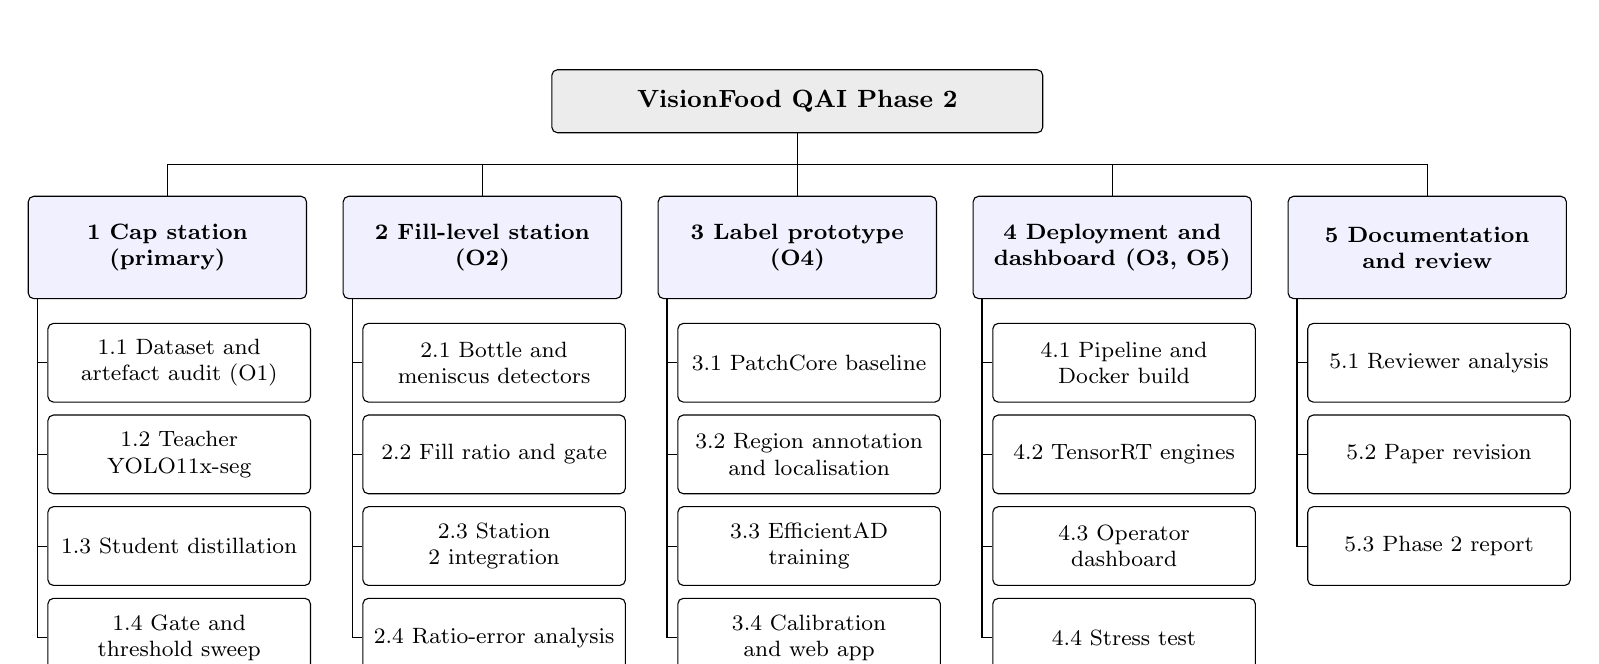
\begin{tikzpicture}[
  wp/.style={blk, fill=blue!6, text width=3.3cm, minimum height=13mm, anchor=north, font={\footnotesize\bfseries\hyphenpenalty=10000}},
  leaf/.style={blk, text width=3.1cm, minimum height=10mm, font={\footnotesize\hyphenpenalty=10000}},
  every node/.style={font=\footnotesize}]
\node[blk, fill=gray!15, text width=6.0cm, font=\small\bfseries] (root) at (8.0,0) {VisionFood QAI Phase 2};
\foreach \i/\t/\x in {1/{1 Cap station\\(primary)}/0, 2/{2 Fill-level station\\(O2)}/4.0, 3/{3 Label prototype\\(O4)}/8.0, 4/{4 Deployment and\\dashboard (O3, O5)}/12.0, 5/{5 Documentation\\and review}/16.0}
  \node[wp] (w\i) at (\x,-1.2) {\t};
\foreach \i in {1,...,5} \draw (root.south) -- ++(0,-0.4) -| (w\i.north);
% each leaf hangs 1.5 mm below the previous one, whatever its height
\def\leaves#1#2{\foreach \lf [count=\k] in {#2} {%
  \ifnum\k=1 \node[leaf, anchor=north west] (#1-\k) at ($(#1.south west)+(0.25,-0.3)$) {\lf};%
  \else \pgfmathtruncatemacro{\prev}{\k-1}\node[leaf, anchor=north west] (#1-\k) at ($(#1-\prev.south west)+(0,-0.15)$) {\lf};\fi}}
\leaves{w1}{{1.1 Dataset and artefact audit (O1)},{1.2 Teacher YOLO11x-seg},{1.3 Student distillation},{1.4 Gate and threshold sweep}}
\leaves{w2}{{2.1 Bottle and meniscus detectors},{2.2 Fill ratio and gate},{2.3 Station 2 integration},{2.4 Ratio-error analysis}}
\leaves{w3}{{3.1 PatchCore baseline},{3.2 Region annotation and localisation},{3.3 EfficientAD training},{3.4 Calibration and web app}}
\leaves{w4}{{4.1 Pipeline and Docker build},{4.2 TensorRT engines},{4.3 Operator dashboard},{4.4 Stress test}}
\leaves{w5}{{5.1 Reviewer analysis},{5.2 Paper revision},{5.3 Phase 2 report}}
\foreach \w/\n in {w1/4,w2/4,w3/4,w4/4,w5/3} {
  \foreach \k in {1,...,\n} \draw ($(\w.south west)+(0.12,0)$) |- (\w-\k.west);
}
\end{tikzpicture}
\end{adjustbox}
\caption[Work breakdown structure]{Work breakdown structure of Phase 2: five work packages and their deliverables.}
\label{fig:wbs}
\end{figure}

\section{Activity Network and Critical Path}
\label{sec:cpm}
Table~\ref{tab:activities} lists the activities with their durations, taken from the bar lengths of the Gantt chart (Figure~\ref{fig:gantt}), and their finish-to-start predecessors. The cap chain follows the dependencies stated in Section~\ref{sec:schedule}: the student cannot be trained before the teacher, the TensorRT engines and stress test need the integrated pipeline, and Station 2 integration needs the station-switching mechanism. A forward pass gives the earliest start (ES) and finish (EF) of each activity, and a backward pass from the project end gives the latest start (LS) and finish (LF); the total float is $\mathrm{LS}-\mathrm{ES}$.

\begin{table}[htbp]
\centering
\caption{Activities, durations, and critical-path analysis (weeks)}
\label{tab:activities}
\setlength{\tabcolsep}{4pt}
\begin{tabularx}{\textwidth}{|L{0.9cm}|X|c|L{2.6cm}|c|c|c|c|c|}
\hline
\textbf{ID} & \textbf{Activity} & \textbf{Dur.} & \textbf{Predecessor} & \textbf{ES} & \textbf{EF} & \textbf{LS} & \textbf{LF} & \textbf{Float} \\ \hline
L1 & PatchCore baseline & 4 & --- & 0 & 4 & 0 & 4 & \textbf{0} \\ \hline
L2 & ROI annotation, crop tools & 1 & L1 & 4 & 5 & 4 & 5 & \textbf{0} \\ \hline
L3 & YOLO11m + SAHI localiser & 2 & L2 & 5 & 7 & 14 & 16 & 9 \\ \hline
L4 & EfficientAD train + calibrate & 2 & L2 & 5 & 7 & 5 & 7 & \textbf{0} \\ \hline
L5 & Grayscale retraining, ONNX & 9 & L4 & 7 & 16 & 7 & 16 & \textbf{0} \\ \hline
L6 & Template matching + web app & 2 & L3, L5 & 16 & 18 & 16 & 18 & \textbf{0} \\ \hline
L7 & ROI\_4 re-annotation + retrain & 1 & L5 & 16 & 17 & 17 & 18 & 1 \\ \hline
C1 & Reviewer analysis, KD plan & 3 & --- & 0 & 3 & 5 & 8 & 5 \\ \hline
C2 & Teacher YOLO11x-seg & 2 & C1 & 3 & 5 & 8 & 10 & 5 \\ \hline
C3 & Student distillation & 2 & C2 & 5 & 7 & 10 & 12 & 5 \\ \hline
C4 & Pipeline + Docker build & 2 & C3 & 7 & 9 & 12 & 14 & 5 \\ \hline
C5 & TRT dynamic batch, stress test & 2 & C4 & 9 & 11 & 14 & 16 & 5 \\ \hline
C6 & Dashboard workstations & 2 & C4 & 9 & 11 & 16 & 18 & 7 \\ \hline
C7 & Gate + threshold sweep & 3 & C3 & 7 & 10 & 15 & 18 & 8 \\ \hline
C8 & Station 2 integration & 2 & C5 & 11 & 13 & 16 & 18 & 5 \\ \hline
R1 & Paper revision, report & 3 & L6, L7, C6, C7, C8 & 18 & 21 & 18 & 21 & \textbf{0} \\ \hline
\end{tabularx}
\end{table}

Figure~\ref{fig:network} draws the activity-on-node network. The critical path is L1 $\rightarrow$ L2 $\rightarrow$ L4 $\rightarrow$ L5 $\rightarrow$ L6 $\rightarrow$ R1, with a length of 21 weeks; this equals the calendar span of the Gantt chart from the start of week 3 to the end of week 23. The label prototype therefore set the project duration, and its longest activity, the nine-week grayscale retraining, was the one that most needed protecting. The cap chain had five weeks of float, which is why its late start in September did not delay the project. In practice the report was started while the last label activities were still running (fast-tracking), which the finish-to-start network does not show.

\begin{figure}[htbp]
\centering
\begin{adjustbox}{max width=\textwidth}
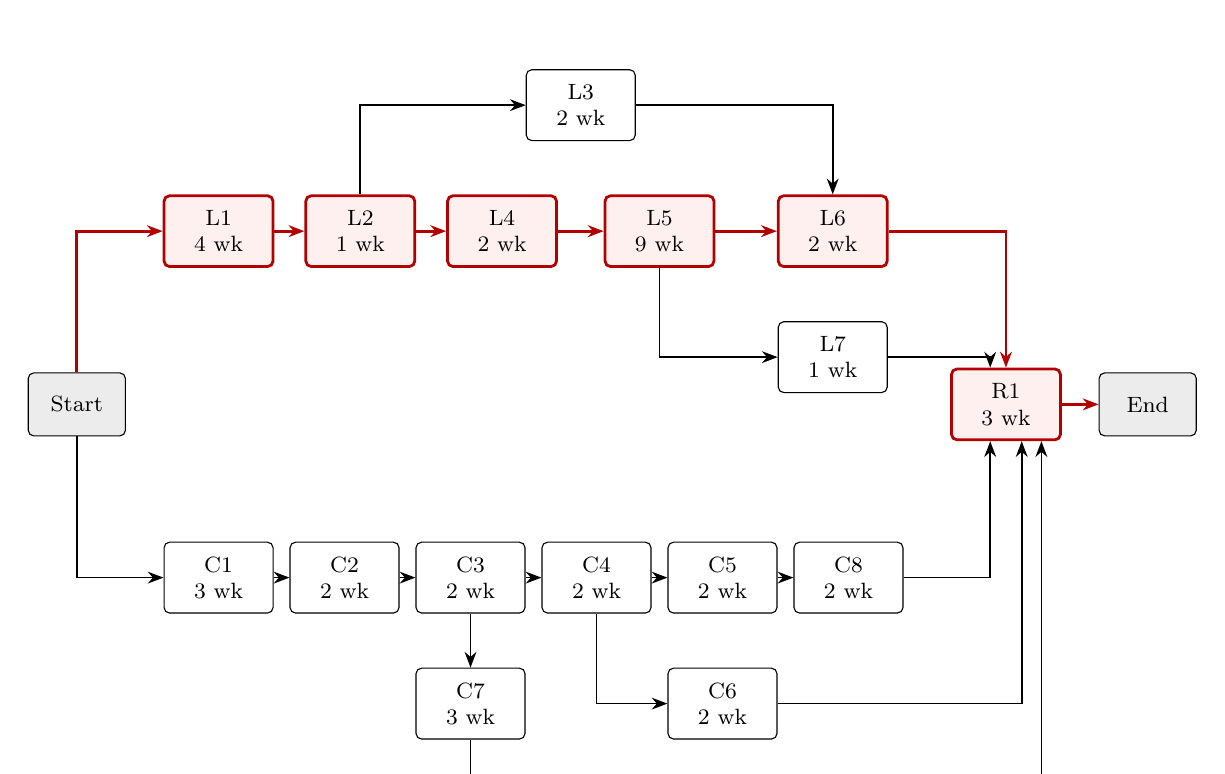
\begin{tikzpicture}[
  act/.style={blk, text width=1.15cm, minimum height=9mm, font=\footnotesize},
  crit/.style={act, draw=red!70!black, line width=1pt, fill=red!6},
  carr/.style={arr, draw=red!70!black, line width=1pt},
  every node/.style={font=\footnotesize}]
\node[blk, fill=gray!15, text width=1.0cm] (st) at (0,-2.2) {Start};
% label track (critical)
\node[crit] (L1) at (1.8,0) {L1\\4 wk};
\node[crit] (L2) at (3.6,0) {L2\\1 wk};
\node[crit] (L4) at (5.4,0) {L4\\2 wk};
\node[crit] (L5) at (7.4,0) {L5\\9 wk};
\node[crit] (L6) at (9.6,0) {L6\\2 wk};
\node[act]  (L3) at (6.4,1.6) {L3\\2 wk};
\node[act]  (L7) at (9.6,-1.6) {L7\\1 wk};
% cap and integration track
\node[act] (C1) at (1.8,-4.4) {C1\\3 wk};
\node[act] (C2) at (3.4,-4.4) {C2\\2 wk};
\node[act] (C3) at (5.0,-4.4) {C3\\2 wk};
\node[act] (C4) at (6.6,-4.4) {C4\\2 wk};
\node[act] (C5) at (8.2,-4.4) {C5\\2 wk};
\node[act] (C8) at (9.8,-4.4) {C8\\2 wk};
\node[act] (C7) at (5.0,-6.0) {C7\\3 wk};
\node[act] (C6) at (8.2,-6.0) {C6\\2 wk};
\node[crit] (R1) at (11.8,-2.2) {R1\\3 wk};
\node[blk, fill=gray!15, text width=1.0cm] (en) at (13.6,-2.2) {End};
% critical arrows
\draw[carr] (st) |- (L1); \draw[carr] (L1) -- (L2); \draw[carr] (L2) -- (L4); \draw[carr] (L4) -- (L5);
\draw[carr] (L5) -- (L6); \draw[carr] (L6) -| (R1); \draw[carr] (R1) -- (en);
% other arrows
\draw[arr] (L2) |- (L3); \draw[arr] (L3) -| (L6);
\draw[arr] (L5) |- (L7); \draw[arr] (L7) -| ([xshift=-2mm]R1.north);
\draw[arr] (st) |- (C1);
\foreach \a/\b in {C1/C2,C2/C3,C3/C4,C4/C5,C5/C8} \draw[arr] (\a) -- (\b);
\draw[arr] (C3) -- (C7); \draw[arr] (C4) |- (C6);
\draw[arr] (C8) -| ([xshift=-2mm]R1.south);
\draw[arr] (C7.south) -- ++(0,-0.6) -| ([xshift=4.5mm]R1.south);
\draw[arr] (C6) -| ([xshift=2mm]R1.south);
\end{tikzpicture}
\end{adjustbox}
\caption[Activity-on-node network]{Activity-on-node network of Phase 2 (IDs as in Table~\ref{tab:activities}). The critical path, in red, runs through the label prototype and the report.}
\label{fig:network}
\end{figure}

\section{Project Schedule and Milestones}
\label{sec:schedule}
\label{subsec:gantt}
Figure~\ref{fig:gantt} shows the Phase 2 timeline from June to November 2026. Work ran in three parallel tracks: the label prototype (June to October), the cap station (September to October), and integration, deployment, and documentation (September to November). The dependencies are: the student cannot be trained before the teacher; TensorRT engines and the stress test require the integrated pipeline; and Station 2 integration requires the station-switching mechanism.

\begin{figure}[htbp]
\centering
\begin{adjustbox}{max width=\textwidth}
\begin{ganttchart}[
    hgrid, vgrid={*3{dotted},*1{solid}},
    x unit=0.55cm, y unit chart=0.52cm, y unit title=0.6cm,
    title height=1,
    bar height=0.55, group height=0.35,
    bar/.append style={fill=blue!35},
    group/.append style={fill=black!70},
    milestone/.append style={fill=red!70},
    bar label font=\footnotesize, group label font=\footnotesize\bfseries,
    milestone label font=\footnotesize\itshape,
    link/.style={->, thick, red!60}
  ]{1}{24}
  \gantttitle{Jun}{4} \gantttitle{Jul}{4} \gantttitle{Aug}{4} \gantttitle{Sep}{4} \gantttitle{Oct}{4} \gantttitle{Nov}{4} \\
  \ganttgroup{Label prototype (O4)}{3}{22} \\
  \ganttbar{PatchCore baseline}{3}{6} \\
  \ganttbar{ROI annotation, crop tools}{8}{8} \\
  \ganttbar[name=yolo]{YOLO11m + SAHI localiser}{8}{9} \\
  \ganttbar[name=ead]{EfficientAD train + calibrate}{9}{10} \\
  \ganttbar{Grayscale retraining, ONNX}{9}{17} \\
  \ganttbar{Template matching + web app}{21}{22} \\
  \ganttbar{ROI\_4 re-annotation + retrain}{22}{22} \\
  \ganttgroup{Cap station (primary)}{12}{21} \\
  \ganttbar{Reviewer analysis, KD plan}{12}{14} \\
  \ganttbar[name=teacher]{Teacher YOLO11x-seg}{13}{14} \\
  \ganttbar[name=student]{Student distillation}{14}{15} \\
  \ganttmilestone{Student model ready}{15} \\
  \ganttbar{Gate + threshold sweep}{19}{21} \\
  \ganttgroup{Integration and deployment}{15}{24} \\
  \ganttbar[name=pipe]{Pipeline + Docker build}{15}{16} \\
  \ganttbar[name=trt]{TRT dynamic batch, stress test}{20}{21} \\
  \ganttbar{Dashboard workstations (O5)}{20}{21} \\
  \ganttbar[name=fill]{Station 2 integration (O2)}{21}{22} \\
  \ganttbar{Paper revision, report}{21}{23} \\
  \ganttmilestone{Phase 2 Review 1}{23}
  \ganttlink{teacher}{student}
  \ganttlink{student}{pipe}
  \ganttlink{pipe}{trt}
  \ganttlink{trt}{fill}
\end{ganttchart}
\end{adjustbox}
\caption[Phase 2 Gantt chart]{Phase 2 Gantt chart (weekly resolution, June--November 2026), reconstructed from the repository commit history. Red arrows mark dependencies; diamonds mark milestones.}
\label{fig:gantt}
\end{figure}

Table~\ref{tab:milestones} lists the milestones, and Table~\ref{tab:plan-actual} compares the Phase 1 plan with what Phase 2 delivered. Several Phase 1 components were deliberately dropped or replaced after the Phase 1 evaluation and the conference reviews; the reasons are recorded alongside.

\begin{table}[htbp]
\centering
\caption{Phase 2 milestones (week numbers as in Figure~\ref{fig:gantt})}
\label{tab:milestones}
\begin{tabularx}{\textwidth}{|L{0.9cm}|X|L{1.4cm}|L{4.2cm}|}
\hline
\textbf{ID} & \textbf{Milestone} & \textbf{Week} & \textbf{Evidence} \\ \hline
M1 & Label baseline evaluated; PatchCore replaced by EfficientAD & 6 & Risk register (Table~\ref{tab:risks}) \\ \hline
M2 & Distilled student model ready & 15 & Table~\ref{tab:kd} \\ \hline
M3 & Integrated pipeline running in Docker & 16 & Section~\ref{sec:system-integration} \\ \hline
M4 & Grayscale label models exported to ONNX & 17 & Table~\ref{tab:label-colour} \\ \hline
M5 & Dynamic-batch engines and stress test complete & 21 & Tables~\ref{tab:latency}, \ref{tab:stress} \\ \hline
M6 & Station 2 integrated; label template matching and web app & 22 & Tables~\ref{tab:fillerr}, \ref{tab:label-roi} \\ \hline
M7 & Phase 2 Review 1 & 23 & This report \\ \hline
\end{tabularx}
\end{table}

\begin{table}[htbp]
\centering
\caption{Phase 1 plan versus Phase 2 outcome}
\label{tab:plan-actual}
\begin{tabularx}{\textwidth}{|L{4.0cm}|L{2.1cm}|X|}
\hline
\textbf{Phase 1 plan item} & \textbf{Status} & \textbf{Phase 2 outcome and reason} \\ \hline
YOLOv8 detector + EfficientViT-M5 / MobileNetV3 cap classifier & Replaced & Distilled YOLO11m-seg student; classifier reached 86.5\% and gave no location (Section~\ref{sec:why-seg}). \\ \hline
Fill-level ratio from water-surface detector & Completed & Formalised with trimming, association, review band, sensitivity analysis, and measured error (O2). \\ \hline
Sub-80\,ms latency per frame & Partly met & 7.4\,ms network time for three views; closed loop 299\,ms because of synchronous storage (O3). \\ \hline
ONNX edge deployment & Extended & TensorRT FP16 engines with ONNX Runtime and PyTorch fallbacks; Docker deployment. \\ \hline
Label misalignment and packaging damage & Re-scoped & Label-defect prototype on the Himalaya NSC tube (O4). \\ \hline
Monte Carlo Dropout uncertainty & Replaced & Deterministic \texttt{UNCERTAIN} band in each gate; no sampling cost at inference. \\ \hline
REMEDY routing, SKU profiles, four package types & Dropped & Not evaluable within Phase 2; reviewers asked for scope to match tested components. \\ \hline
React dashboard, inspection history, PDF shift report & Partly met & Dashboard, audit table, replay, review queue, and CSV export delivered; PDF shift report not implemented (O5). \\ \hline
\end{tabularx}
\end{table}

\section{Responsibility Assignment Matrix}
\label{sec:raci}
Table~\ref{tab:raci} assigns each work package of Figure~\ref{fig:wbs} using the RACI convention: \textbf{R}esponsible (does the work), \textbf{A}ccountable (approves it), \textbf{C}onsulted, and \textbf{I}nformed. The guide is accountable for every package.

\begin{table}[htbp]
\centering
\caption{Responsibility assignment matrix (R: responsible, A: accountable, C: consulted, I: informed)}
\label{tab:raci}
\begin{tabularx}{\textwidth}{|X|c|c|c|c|}
\hline
\textbf{Work package} & \textbf{Shreyas} & \textbf{Sushanth} & \textbf{Ullas} & \textbf{Guide} \\ \hline
1 Cap station (dataset audit, teacher, student, gate) & C & R & C & A \\ \hline
2 Fill-level station (detectors, ratio, gate, integration) & C & R & R & A \\ \hline
3 Label prototype (baselines, localisation, EfficientAD, web app) & R & I & R & A \\ \hline
4 Deployment and dashboard (pipeline, engines, dashboard, stress test) & C & R & C & A \\ \hline
5 Documentation and review (reviewer analysis, paper, report) & R & R & R & A \\ \hline
\end{tabularx}
\end{table}

\section{Risk Register and Mitigation}
\label{sec:risk}
Table~\ref{tab:risks} lists the risks identified during Phase 2, the mitigation applied, and the evidence that the plan was adjusted.

\begin{table}[htbp]
\centering
\caption{Risk register with mitigation and evidence of adjustment}
\label{tab:risks}
\begin{tabularx}{\textwidth}{|L{3.6cm}|L{1.6cm}|X|}
\hline
\textbf{Risk} & \textbf{Impact} & \textbf{Mitigation and evidence of adjustment} \\ \hline
Cap classifier below target (86.5\%) & High & Switched to segmentation; distilled a large teacher into a deployable student (Sections~\ref{sec:why-seg}, \ref{sec:kd-impl}). \\ \hline
Large model too slow for line rate & High & Feature distillation (2.8$\times$ fewer parameters) and TensorRT FP16 engines; latency measured per stage (Table~\ref{tab:latency}). \\ \hline
TensorRT static batch silently fell back to single-image inference & Medium & Rebuilt engines with a dynamic batch profile, added batched warm-up checks and versioned engine files (September--October 2026). \\ \hline
Two stations exceeding one GPU's memory & Medium & Lazy loading of Station 2 and explicit unload/load on station switch, guarded by locks. \\ \hline
PatchCore too slow for the label scans & Medium & Replaced by EfficientAD-Medium after the June--July baseline. \\ \hline
Down-scaled 8000\,px scans hid label regions from the detector & Medium & Tried YOLO11m with SAHI tiling (July); replaced by deterministic template matching, which located all four regions on all 120 scans (October). \\ \hline
White label background caused false alarms in colour models & Medium & Retrained on grayscale crops; recall on ROI\_1--3 rose to 93--94\% (Table~\ref{tab:label-roi}). \\ \hline
Noisy ROI\_4 annotations & Medium & Re-annotated and retrained ROI\_4 on combined data; still open (57.9\% precision). \\ \hline
Synchronous audit storage limits throughput & Medium & Measured and reported (Table~\ref{tab:stress}); asynchronous writes planned as future work. \\ \hline
Conference rejection (CSITSS 2026) & Medium & Reviewer comments mapped to concrete changes; paper rewritten around measured stations. \\ \hline
\end{tabularx}
\end{table}

\section{Resource and Cost Estimate}
\label{sec:cost}
Table~\ref{tab:resources} lists the resources used in Phase 2, their quantity or usage, and how they were obtained. All software is open source or free to use, all public datasets are under CC BY 4.0, so the project incurred no licence or dataset cost. The largest compute item is the training of the two cap models, 17.5 GPU-hours in total.

\begin{table}[htbp]
\centering
\caption{Resources used and their source}
\label{tab:resources}
\begin{tabularx}{\textwidth}{|L{3.5cm}|X|L{3.7cm}|}
\hline
\textbf{Resource} & \textbf{Quantity or usage} & \textbf{Source and cost} \\ \hline
GPU workstation (RTX A5000, 24\,GB) & Teacher training 12.2\,h; student training 5.3\,h; all latency measurements & Existing equipment; no purchase for Phase 2 \\ \hline
Development PCs & Coding, dashboard development, CPU fallback tests & Students' own machines \\ \hline
Deep learning and deployment software & PyTorch, Ultralytics, TensorRT, ONNX Runtime, Anomalib, FastAPI, React, Docker & Open source or free licences; no cost \\ \hline
Public datasets & Cap segmentation set, bottle and meniscus sets (Table~\ref{tab:datasets}) & Roboflow Universe, CC BY 4.0; no cost \\ \hline
Label scans & 120 Himalaya NSC tube scans & Industrial partner; not redistributed \\ \hline
Annotation and hosting & Roboflow, LabelImg, GitHub & Free tiers; no cost \\ \hline
\end{tabularx}
\end{table}

For a plant adopting the system, the recurring cost is limited to the cameras, lighting, and one workstation-class NVIDIA GPU per line; the software stack carries no licence fee.

%======================================================================
\chapter{Implementation}
\label{ch:impl}

This chapter gives the algorithms behind each station, the loss functions used in training, the decision rules used at inference, the way the modules are integrated and deployed, and the tests that verify them. Long code listings are placed in Appendix~\ref{appendix:code}.

\section{Algorithm Implementation}
\label{sec:algorithm-implementation}

\subsection{Notation}
\label{sec:notation}
Table~\ref{tab:notation} collects the symbols used throughout this chapter.

\begin{table}[htbp]
\centering
\caption{Notation}
\label{tab:notation}
\begin{tabularx}{\textwidth}{|L{3.4cm}|X|}
\hline
\textbf{Symbol} & \textbf{Meaning} \\ \hline
$I_v \in \mathbb{R}^{H\times W\times 3}$ & Image from camera view $v\in\{1,2,3\}$ \\ \hline
$\mathcal{D}_v$ & Detections $\{(b_i,c_i,s_i,M_i)\}$ in view $v$: box $b_i=(x_1,y_1,x_2,y_2)$, class $c_i$, score $s_i$, mask $M_i$ \\ \hline
$\mathcal{C}$, $\mathcal{C}_d$ & Cap classes $\mathcal{C}=\{\text{good},\text{damaged},\text{misplaced},\text{no},\text{open},\text{wet}\}$; defect classes $\mathcal{C}_d=\mathcal{C}\setminus\{\text{good}\}$ \\ \hline
$F^T_\ell, F^S_\ell$ & Teacher and student feature maps at distillation site $\ell$ \\ \hline
$\phi_\ell$ & Learned $1{\times}1$ convolutional projector at site $\ell$ (training only) \\ \hline
$\alpha(t)$ & Distillation weight at epoch $t$ \\ \hline
$\tau_p,\tau_d,\tau_u$ & Cap gate thresholds: pass, defect, uncertain floor \\ \hline
$b$, $w$ & Bottle box $b=(x^b_1,y^b_1,x^b_2,y^b_2)$ and associated meniscus (water-surface) box $w$ \\ \hline
$h, h'$ & Bottle box height before and after trimming \\ \hline
$y_w$ & Meniscus height (box mid-line, clamped) \\ \hline
$\Rfill$ & Fill ratio, $0$ = empty, $1$ = full \\ \hline
$\theta_u,\theta_o,\beta,c_{\min}$ & Underfill and overfill limits, review half-band, minimum meniscus confidence \\ \hline
$T_k$, $\rho_k(x,y)$ & Template of label region $k$ and its normalised cross-correlation map \\ \hline
$A_k$, $\sigma_k$, $\tau_k$ & Anomaly map, anomaly score, and threshold of label region $k$ \\ \hline
\end{tabularx}
\end{table}

\subsection{Segmentation network}
\label{sec:seg-impl}
Both cap networks (teacher YOLO11x-seg and student YOLO11m-seg) share the YOLO11 segmentation design~\cite{jocher2024}. For an input image the backbone and neck produce feature maps at strides 8, 16, and 32. At every anchor point the head predicts (i) class logits $z\in\mathbb{R}^{|\mathcal{C}|}$, (ii) a discretised distribution over the four box-edge offsets, and (iii) a mask-coefficient vector $\mathbf{m}\in\mathbb{R}^{K}$. A separate prototype branch predicts $K=32$ full-image prototypes $P\in\mathbb{R}^{K\times H_p\times W_p}$. Following YOLACT~\cite{bolya2019}, the mask of instance $i$ is
\begin{equation}
    M_i = \sigma\!\left(\sum_{k=1}^{K} m_{i,k}\,P_k\right)\odot \mathbb{1}[b_i],
    \label{eq:mask}
\end{equation}
where $\sigma$ is the logistic function and $\mathbb{1}[b_i]$ crops the mask to the predicted box. Because the prototypes are shared, the per-instance cost of a mask is one $K$-dimensional linear combination.

\subsection{Supervised training loss}
The base loss is the Ultralytics segmentation loss, a weighted sum of four terms:
\begin{equation}
    \mathcal{L}_{\text{YOLO}} = \lambda_{\text{box}}\,\mathcal{L}_{\text{CIoU}} + \lambda_{\text{box}}\,\mathcal{L}_{\text{seg}} + \lambda_{\text{cls}}\,\mathcal{L}_{\text{BCE}} + \lambda_{\text{dfl}}\,\mathcal{L}_{\text{DFL}},
    \label{eq:yololoss}
\end{equation}
where $\mathcal{L}_{\text{CIoU}}$ is the complete-IoU box loss, $\mathcal{L}_{\text{seg}}$ is the per-pixel binary cross-entropy between predicted and ground-truth masks (normalised by box area and weighted by the box gain, as implemented in Ultralytics), $\mathcal{L}_{\text{BCE}}$ is the binary cross-entropy classification loss, and $\mathcal{L}_{\text{DFL}}$ is the distribution focal loss on the edge distributions. Positive anchors are chosen by a task-aligned assigner. We used $\lambda_{\text{box}}=7.5$, $\lambda_{\text{dfl}}=1.5$, and $\lambda_{\text{cls}}=4.0$.

The classification gain was raised from the default $0.5$ to compensate for class imbalance. With $n_c$ training instances of class $c$, the majority-to-class ratio averaged over classes is
\begin{equation}
    \bar{r} = \frac{1}{|\mathcal{C}|}\sum_{c\in\mathcal{C}}\frac{\max_{c'} n_{c'}}{n_c} = 6.29,
    \label{eq:imb}
\end{equation}
and the gain was set to $\min(\bar r, 4.0)=4.0$. This is a single scalar: it strengthens the classification signal relative to localisation but does not re-weight classes individually, unlike class-balanced or focal losses~\cite{cui2019,lin2017focal}.

\subsection{Teacher--student feature distillation}
\label{sec:kd-impl}

\noindent\textbf{General form.} A distillation objective for a detector can combine a response term, a box term, and a feature term:
\begin{equation}
    \mathcal{L}_{\text{distill}} = \alpha\,\mathcal{L}^{\text{KD}}_{\text{cls}} + \beta\,\mathcal{L}^{\text{KD}}_{\text{box}} + \gamma\,\mathcal{L}^{\text{KD}}_{\text{feat}}.
    \label{eq:distill-general}
\end{equation}
The response (logit) term matches temperature-softened class distributions~\cite{hinton2015},
\begin{equation}
    \mathcal{L}^{\text{KD}}_{\text{cls}} = \mathcal{T}^2\,\mathrm{KL}\!\left(\mathrm{softmax}(z^T/\mathcal{T})\,\Big\|\,\mathrm{softmax}(z^S/\mathcal{T})\right),
    \label{eq:logitkd}
\end{equation}
with temperature $\mathcal{T}>1$; the box term matches the teacher's edge distributions in the same way; and the feature term matches intermediate representations through learned projectors~\cite{romero2015}.

\noindent\textbf{Configuration used.} For bottle caps the decisive evidence (droplets, dents, a thread gap) covers a small part of the cap, and the teacher and student make near-identical final predictions on most images. Matching outputs alone would mainly transfer \emph{what} to predict. We therefore set $\alpha=\beta=0$ and distil features only, adding them to the supervised loss of Eq.~\eqref{eq:yololoss}:
\begin{equation}
    \mathcal{L} = \mathcal{L}_{\text{YOLO}} + \alpha(t)\sum_{\ell\in\mathcal{S}} \frac{1}{C_\ell H_\ell W_\ell}\left\| \widehat{F^T_\ell} - \widehat{\phi_\ell(F^S_\ell)} \right\|_2^2 ,
    \label{eq:kd}
\end{equation}
where $\mathcal{S}=\{\text{C3k2},\ \text{SPPF},\ \text{C2PSA}\}$ are the three distillation sites, $C_\ell\times H_\ell\times W_\ell$ is the teacher feature shape at site $\ell$, and $\widehat{\cdot}$ denotes channel-wise $L_2$ normalisation at every spatial position $(x,y)$:
\begin{equation}
    \widehat{F}(x,y) = \frac{F(x,y)}{\|F(x,y)\|_2+\epsilon}.
    \label{eq:l2norm}
\end{equation}

\noindent\textbf{Why normalise.} For unit vectors $\hat a$ and $\hat b$,
\begin{equation}
    \|\hat a-\hat b\|_2^2 = 2\left(1-\cos(a,b)\right),
    \label{eq:cosine}
\end{equation}
so the feature term of Eq.~\eqref{eq:kd} is a mean cosine distance between teacher and projected student features. It depends on the \emph{direction} of each feature vector and not on its magnitude, so the large, uniform background, where activations are strong but uninformative, cannot dominate the loss. This addresses the background-swamping problem noted for detector distillation~\cite{wang2019fgfi}.

\noindent\textbf{Distillation sites.} The three sites were chosen for what they carry. C3k2 at the backbone output holds edge and texture features, including thread and ridge geometry. SPPF at the backbone--neck transition holds multi-scale pooled context, which helps fine cues survive down-sampling. C2PSA holds the teacher's spatial attention, which transfers \emph{where} the fine defect evidence lies. The student and teacher feature maps have the same spatial size at each site because the two models share strides; only the channel widths differ. The projectors $\phi_\ell$ are $1{\times}1$ convolutions that lift student channels to teacher width ($256\rightarrow512$ and $512\rightarrow1024$).

\noindent\textbf{Schedule.} The distillation weight ramps linearly over the first 20 epochs:
\begin{equation}
    \alpha(t) = \alpha_0 + (\alpha_1-\alpha_0)\,\min\!\left(\frac{t}{t_r},1\right),\qquad \alpha_0=0.05,\ \alpha_1=0.5,\ t_r=20.
    \label{eq:ramp}
\end{equation}
Early epochs are dominated by the supervised loss, so the student first learns basic detection; the alignment pressure then reaches full strength. Teacher features are detached, so no gradient reaches the teacher. The projectors exist only in training and are discarded before export, so distillation adds no inference cost. Algorithm~\ref{alg:kd} summarises one training step.

\begin{algorithm}[htbp]
\caption{One training step of feature distillation}
\label{alg:kd}
\begin{algorithmic}[1]
\Require Batch $(X,Y)$, frozen teacher $f^T$, student $f^S$, projectors $\{\phi_\ell\}$, epoch $t$
\Ensure Updated student and projector parameters
\State Register forward hooks on sites $\ell\in\mathcal{S}$ in $f^T$ and $f^S$
\State $\{F^T_\ell\} \gets f^T(X)$ \textbf{without gradient} \Comment{teacher frozen}
\State $(\hat Y, \{F^S_\ell\}) \gets f^S(X)$
\State $\mathcal{L}_{\text{YOLO}} \gets$ Eq.~\eqref{eq:yololoss} on $(\hat Y, Y)$
\State $\mathcal{L}_{\text{feat}} \gets 0$
\For{each site $\ell\in\mathcal{S}$}
    \State $G \gets \phi_\ell(F^S_\ell)$ \Comment{$1{\times}1$ projection to teacher width}
    \State $\mathcal{L}_{\text{feat}} \gets \mathcal{L}_{\text{feat}} + \mathrm{MSE}\big(\mathrm{norm}(F^T_\ell),\ \mathrm{norm}(G)\big)$ \Comment{Eq.~\eqref{eq:l2norm}}
\EndFor
\State $\mathcal{L} \gets \mathcal{L}_{\text{YOLO}} + \alpha(t)\,\mathcal{L}_{\text{feat}}$ \Comment{Eq.~\eqref{eq:ramp}}
\State Back-propagate $\mathcal{L}$; update $f^S$ and $\{\phi_\ell\}$ with AdamW
\end{algorithmic}
\end{algorithm}

\noindent\textbf{Training configuration.} Table~\ref{tab:train-config} lists the settings. The teacher was trained first on the same data and settings at batch 16 for the full 150 epochs and then frozen. The student was initialised from COCO weights~\cite{lin2014coco}.

\begin{table}[htbp]
\centering
\caption{Training configuration of the cap teacher and student}
\label{tab:train-config}
\begin{tabularx}{\textwidth}{|L{3.6cm}|X|X|}
\hline
\textbf{Setting} & \textbf{Teacher (YOLO11x-seg)} & \textbf{Student (YOLO11m-seg)} \\ \hline
Parameters / GFLOPs @640 & 62.06\,M / 297.4 & 22.34\,M / 113.0 \\ \hline
Input size, batch & 640\,px, 16 & 640\,px, 32 \\ \hline
Optimiser & \multicolumn{2}{p{10.4cm}|}{AdamW, lr $10^{-3}\rightarrow10^{-5}$ cosine, 5 warm-up epochs, weight decay $5{\times}10^{-4}$} \\ \hline
Loss gains & \multicolumn{2}{p{10.4cm}|}{box 7.5, DFL 1.5, cls 4.0} \\ \hline
Augmentation & \multicolumn{2}{p{10.4cm}|}{mosaic (off for last 10 epochs), copy-paste 0.5, mixup 0.15, rotation $\pm15^\circ$, translate 0.1, scale 0.5, flips (v 0.3, h 0.5), HSV jitter, RandAugment, erasing 0.4} \\ \hline
Distillation & --- & Eq.~\eqref{eq:kd}, sites C3k2/SPPF/C2PSA \\ \hline
Epochs (best) & 150 (139) & 126, early stop, patience 30 (96) \\ \hline
Wall-clock time & 12.2\,h & 5.3\,h \\ \hline
Hardware & \multicolumn{2}{p{10.4cm}|}{NVIDIA RTX A5000 24\,GB; mixed precision; seed 42} \\ \hline
\end{tabularx}
\end{table}

\subsection{Asymmetric multi-view quality gate}
\label{sec:gate-impl}
The cap engine runs with a confidence floor of $0.35$. Let $\mathcal{D}_v$ be the detections of view $v$ above the floor, $(c^\star_v, s^\star_v)$ the class and score of the top detection, and
\begin{equation}
    s^{d}_v = \max\{s_i : (b_i,c_i,s_i,M_i)\in\mathcal{D}_v,\ c_i\in\mathcal{C}_d\}
\end{equation}
the strongest defect score ($-\infty$ if none). The per-view verdict is
\begin{equation}
    g(v)=\begin{cases}
    \texttt{FAILED} & \mathcal{D}_v=\emptyset\\
    \texttt{REJECT} & s^{d}_v \geq \tau_d\\
    \texttt{PASS} & c^\star_v=\text{good},\ s^\star_v\geq\tau_p\\
    \texttt{UNCERTAIN} & \text{otherwise}
    \end{cases}
    \label{eq:gate}
\end{equation}
with defaults $\tau_d=0.45$, $\tau_p=0.75$, and an uncertain floor $\tau_u=0.40$ that labels a good-cap score in $[\tau_u,\tau_p)$ as borderline in the audit record. The bottle verdict aggregates the views with a strict precedence:
\begin{equation}
    G = \begin{cases}
    \texttt{REJECT} & \exists v: g(v)=\texttt{REJECT}\\
    \texttt{INSPECTION\_FAILED} & \text{else } \exists v: g(v)=\texttt{FAILED}\\
    \texttt{UNCERTAIN} & \text{else } \exists v: g(v)=\texttt{UNCERTAIN}\\
    \texttt{PASS} & \text{otherwise.}
    \end{cases}
    \label{eq:agg}
\end{equation}
\texttt{REJECT} and \texttt{INSPECTION\_FAILED} fire the actuator; \texttt{UNCERTAIN} goes to the review queue without ejection. The thresholds are asymmetric by design ($\tau_d<\tau_p$): the bar for rejecting is lower than the bar for passing, so a doubtful cap is never passed automatically. All three thresholds can be changed at run time from the dashboard.

\subsection{Station 1 inspection cycle}
\label{sec:cap-cycle}
Algorithm~\ref{alg:capcycle} gives the complete Station 1 cycle for one bottle, from the three camera frames to the stored record and the dashboard update. It runs inside the cap service and calls the network of Section~\ref{sec:seg-impl} and the gate of Eqs.~\eqref{eq:gate}--\eqref{eq:agg}. The three views share one batched forward pass; if the loaded engine rejects a batch, the views are run one at a time so that the inspection still completes. Detections are taken from each view's own result, so NMS never mixes boxes from different cameras.

\begin{algorithm}[htbp]
\caption{Station 1 cap inspection cycle}
\label{alg:capcycle}
\begin{algorithmic}[1]
\Require Frames $\{I_v\}$ for $v\in\{\text{front},\text{rear},\text{side}\}$, cap engine $f$, thresholds $\tau_p,\tau_d,\tau_u$, confidence floor $0.35$
\Ensure Bottle verdict $G$, actuator flag, audit record
\State acquire the inference lock \Comment{one inspection per engine at a time}
\State $f \gets$ current engine reference, read once \Comment{a station switch may unload it}
\State $X \gets [I_{\text{front}}, I_{\text{rear}}, I_{\text{side}}]$, each resized to $640$\,px
\State $\{R_v\} \gets f(X)$ with confidence $\geq0.35$ \Comment{one batched pass}
\If{the engine rejects the batch}
    \State $R_v \gets f(I_v)$ for each view in turn \Comment{sequential fallback}
\EndIf
\For{each view $v$}
    \State $\mathcal{D}_v \gets$ boxes, classes, scores, and masks of $R_v$, rescaled to $I_v$ \Comment{per-view NMS}
    \State $g(v) \gets$ Eq.~\eqref{eq:gate} on $\mathcal{D}_v$
\EndFor
\State $G \gets$ Eq.~\eqref{eq:agg} on $\{g(v)\}$
\State actuator $\gets$ ($G=\texttt{REJECT}$ \textbf{or} $G=\texttt{INSPECTION\_FAILED}$)
\State write raw frames and YOLO labels to the bottle bundle; insert the \texttt{inspections} row and one \texttt{defect\_events} row per defect (SQLite, WAL)
\State render the per-view overlays and broadcast the result on the WebSocket stream
\State release the inference lock
\State \Return $G$, actuator, record
\end{algorithmic}
\end{algorithm}

\subsection{Fill-level estimation}
\label{sec:fill-impl}

\noindent\textbf{Stage 1: bottle localisation.} The bottle detector runs at confidence $\geq0.25$ and the highest-scoring \texttt{bottle} box $b$ is kept. If none is found the frame is treated as a conveyor gap.

\noindent\textbf{Stage 2: meniscus association and ratio.} The meniscus detector runs on the full frame at confidence $\geq0.15$. A candidate surface box $w=(x^w_1,y^w_1,x^w_2,y^w_2)$ is associated with the bottle when
\begin{equation}
    x^b_1 \leq \tfrac{1}{2}(x^w_1+x^w_2) \leq x^b_2
    \quad\wedge\quad
    \left(y^w_1\in[y^b_1,y^b_2] \ \vee\ y^w_2\in[y^b_1,y^b_2]\right),
    \label{eq:assoc}
\end{equation}
and among associated candidates the highest-scoring one is kept. With $h=y^b_2-y^b_1$, the bottle box is trimmed to remove detector padding at the cap and the base:
\begin{equation}
    y'_1 = y^b_1+\lfloor 0.03h\rfloor,\qquad y'_2 = y^b_2-\lfloor 0.02h\rfloor,\qquad h'=y'_2-y'_1 .
    \label{eq:trim}
\end{equation}
The meniscus height is the mid-line of the surface box, clamped to the trimmed bottle,
\begin{equation}
    y_w = \min\!\Big(y'_2,\ \max\!\big(y'_1,\ \lfloor (y^w_1+y^w_2)/2\rfloor\big)\Big),
\end{equation}
and the fill ratio is (image $y$ grows downwards)
\begin{equation}
    \Rfill = \frac{y'_2-y_w}{h'}\in[0,1].
    \label{eq:rfill}
\end{equation}
Figure~\ref{fig:fill-geom} illustrates the geometry.

\begin{figure}[htbp]
\centering
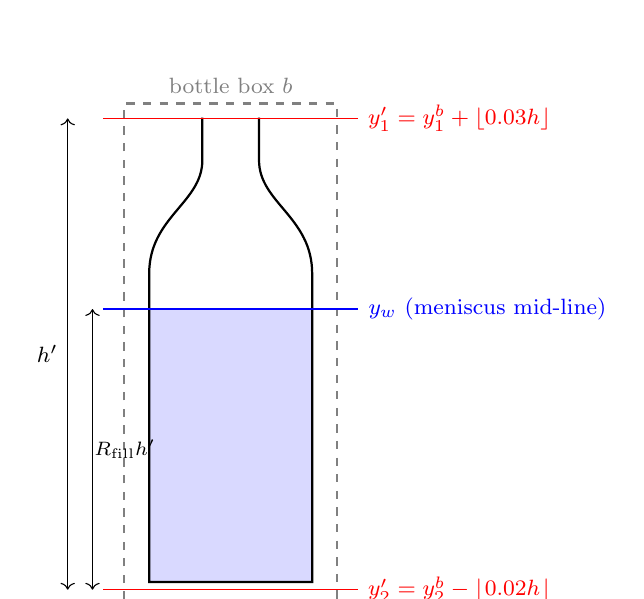
\begin{tikzpicture}[scale=0.9, every node/.style={font=\footnotesize}]
\draw[gray, dashed, thick] (0,0) rectangle (3,7);
\node[gray, above] at (1.5,7) {bottle box $b$};
\fill[blue!15] (0.35,0.25) rectangle (2.65,4.1);
\draw[thick] (1.1,6.8) -- (1.1,6.2) .. controls (1.1,5.6) and (0.35,5.4) .. (0.35,4.6) -- (0.35,0.25) -- (2.65,0.25) -- (2.65,4.6) .. controls (2.65,5.4) and (1.9,5.6) .. (1.9,6.2) -- (1.9,6.8);
\draw[red] (-0.3,6.79) -- (3.3,6.79) node[right]{$y'_1=y^b_1+\lfloor0.03h\rfloor$};
\draw[red] (-0.3,0.14) -- (3.3,0.14) node[right]{$y'_2=y^b_2-\lfloor0.02h\rfloor$};
\draw[blue, thick] (-0.3,4.1) -- (3.3,4.1) node[right]{$y_w$ (meniscus mid-line)};
\draw[<->] (-0.8,0.14) -- node[left]{$h'$} (-0.8,6.79);
\draw[<->] (-0.45,0.14) -- node[right, xshift=-1mm]{\scriptsize$\Rfill h'$} (-0.45,4.1);
\end{tikzpicture}
\caption{Fill-ratio geometry: trimmed bottle box (red) and meniscus mid-line (blue).}
\label{fig:fill-geom}
\end{figure}

\noindent\textbf{Stage 3: three-class fill state and gate.} The ratio is mapped to a fill state with the configurable limits $\theta_u=0.40$ and $\theta_o=0.85$:
\begin{equation}
    \text{state}(\Rfill) = \begin{cases}
    \text{underfill} & \Rfill<\theta_u\\
    \text{overfill} & \Rfill>\theta_o\\
    \text{acceptable} & \text{otherwise.}
    \end{cases}
    \label{eq:fillstate}
\end{equation}
These limits are engineering defaults, not regulatory values; they are read from a single configuration source so that a plant can set them per product, and the gate, the overlay ruler, and the health endpoint all read the same values. Algorithm~\ref{alg:fillgate} applies a review band of half-width $\beta=0.02$ around each limit when the meniscus confidence $c_w$ is below $c_{\min}=0.50$.

\begin{algorithm}[htbp]
\caption{Fill gate}
\label{alg:fillgate}
\begin{algorithmic}[1]
\Require Bottle box $b$ (or none), meniscus box $w$ with confidence $c_w$ (or none), $\Rfill$
\Ensure Verdict $V$ and actuator flag
\If{no bottle}
    \State \Return \texttt{INSPECTION\_FAILED}, no actuation \Comment{conveyor gap}
\ElsIf{no associated meniscus}
    \State \Return \texttt{REJECT} \Comment{empty or opaque}
\ElsIf{$\min_{\theta\in\{\theta_u,\theta_o\}}|\Rfill-\theta|\leq\beta$ \textbf{and} $c_w<c_{\min}$}
    \State \Return \texttt{UNCERTAIN} \Comment{borderline and weakly detected}
\ElsIf{state$(\Rfill)\neq$ acceptable}
    \State \Return \texttt{REJECT} (underfill or overfill)
\Else
    \State \Return \texttt{PASS}
\EndIf
\end{algorithmic}
\end{algorithm}

\noindent\textbf{Sensitivity.} Differentiating Eq.~\eqref{eq:rfill} gives
\begin{equation}
    \frac{\partial \Rfill}{\partial y_w} = -\frac{1}{h'},\qquad
    \frac{\partial \Rfill}{\partial y'_1} = \frac{\Rfill}{h'},\qquad
    \frac{\partial \Rfill}{\partial y'_2} = \frac{1-\Rfill}{h'}.
    \label{eq:sens}
\end{equation}
An error of $\delta$ pixels in the meniscus shifts the ratio by $\delta/h'$. For the median test bottle ($h=620$\,px, $h'\approx589$\,px) one pixel is $0.0017$, so the $\pm0.02$ review band corresponds to about 12 pixels. If the three edge errors are independent with standard deviations $\sigma_w$, $\sigma_1$, and $\sigma_2$, first-order propagation gives
\begin{equation}
    \sigma_R \approx \frac{1}{h'}\sqrt{\sigma_w^2 + \Rfill^2\sigma_1^2 + (1-\Rfill)^2\sigma_2^2}.
    \label{eq:prop}
\end{equation}
Using the mid-line of the surface box rather than one of its edges halves the effect of a symmetric error in the box height, because both edges move by equal and opposite amounts.

\noindent\textbf{Why a rule rather than a classifier.} A MobileNetV3 fill-level classifier was also trained during the project and reached 93.10\% test accuracy (135 of 145 images). It is not used in the deployed path: a classifier returns a label but no measurement, so its limits cannot be moved per product without retraining, and its errors cannot be traced to a pixel position. The geometric rule exposes $\Rfill$, its limits, and its sensitivity.

\subsection{Label-defect prototype}
\label{sec:label-impl}

\noindent\textbf{Preprocessing and localisation.} The scan $I$ is converted to grayscale. For each region $k$ a full-resolution template $T_k$ was cut from one clean reference scan. The match score at offset $(x,y)$ is the zero-mean normalised cross-correlation~\cite{lewis1995}
\begin{equation}
    \rho_k(x,y) = \frac{\sum_{u,v}\tilde T_k(u,v)\,\tilde I(x+u,y+v)}
    {\sqrt{\sum_{u,v}\tilde T_k(u,v)^2\ \sum_{u,v}\tilde I(x+u,y+v)^2}}\in[-1,1],
    \label{eq:ncc}
\end{equation}
where $\tilde{\cdot}$ subtracts the mean over the template window. Search is coarse-to-fine: Eq.~\eqref{eq:ncc} is evaluated on the image and template down-sampled by 4, and the peak is refined at full resolution within $\pm12$ pixels. Because the label wraps around the tube, each region occurs twice; candidates whose region would extend past the scan are discarded so that the complete occurrence is kept. A region is \emph{missing} when its best score is below $0.45$. If two located regions overlap by more than 10\% of the smaller one, the lower-scoring region is searched again with the other's area excluded, so that a damaged region is reported missing instead of silently landing on a neighbour.

\noindent\textbf{ROI cropping.} Each located region is cropped and rotated $90^\circ$ clockwise into the upright orientation in which the anomaly models were trained, then resized to $256{\times}256$. For the grayscale models the single channel is replicated to three channels.

\noindent\textbf{Model routing and anomaly scoring.} Each crop is routed to the EfficientAD-Medium model of its region~\cite{batzner2024}. EfficientAD has a frozen pretrained teacher network $\mathcal{T}$, a student $\mathcal{S}$ with two output groups, and an autoencoder $\mathcal{A}$, all trained only on good crops. For a crop $x$ the two anomaly maps are
\begin{equation}
    A^{\text{ST}}(x) = \frac{1}{C}\sum_{c}\big(\mathcal{T}_c(x)-\mathcal{S}^{\text{st}}_c(x)\big)^2,\qquad
    A^{\text{AE}}(x) = \frac{1}{C}\sum_{c}\big(\mathcal{A}_c(x)-\mathcal{S}^{\text{ae}}_c(x)\big)^2,
\end{equation}
the first sensitive to local texture anomalies and the second to logical or layout anomalies. Each map is normalised with statistics from good validation crops and the two are averaged into $A_k(x)$. The region score is the mean of the map,
\begin{equation}
    \sigma_k = \frac{1}{|\Omega|}\sum_{p\in\Omega} A_k(x)_p ,
    \label{eq:roiscore}
\end{equation}
and the label verdict is
\begin{equation}
    \text{label} = \begin{cases}
    \texttt{FAIL} & \exists k:\ \sigma_k>\tau_k \ \text{or region } k \text{ missing}\\
    \texttt{PASS} & \text{otherwise.}
    \end{cases}
    \label{eq:labelrule}
\end{equation}

\noindent\textbf{Threshold calibration.} Defective crops are used only to set thresholds. Two strategies were used: a recall-targeted threshold at the 5th percentile of defective-crop scores, which guarantees that at least 95\% of the calibration defects exceed it, and an F1-optimal sweep. For the final ROI\_4 model the crops were split 80/20 with a fixed seed; the threshold was set on the calibration part for a 95\% recall target and evaluated once on the remaining part.

\noindent\textbf{Explainability.} The upload-and-inspect application overlays the pixels of $A_k$ that exceed $\tau_k$, finds up to three connected hot regions, and reports for each how much it adds to $\sigma_k$ and what the region would score if that area were replaced by the crop median. If the counterfactual score falls below the threshold, that area alone causes the rejection. Algorithm~\ref{alg:label} summarises the prototype.

\begin{algorithm}[htbp]
\caption{Label-defect inspection}
\label{alg:label}
\begin{algorithmic}[1]
\Require Scan $I$, templates $\{T_k\}$, models $\{\mathcal{M}_k\}$, thresholds $\{\tau_k\}$
\Ensure Label verdict, per-region scores and heatmaps
\State $G \gets \mathrm{gray}(I)$; $G_4 \gets \mathrm{downsample}(G,4)$
\For{$k=1$ \textbf{to} $4$}
    \State $(x_k,y_k) \gets \arg\max \rho_k$ on $G_4$, complete occurrences only; refine on $G$ within $\pm12$\,px
    \State mark region $k$ missing if $\rho_k<0.45$
\EndFor
\State resolve overlaps $>10\%$ by re-searching the lower-scoring region
\For{each found region $k$}
    \State $x \gets \mathrm{resize}(\mathrm{rot90}(\mathrm{crop}(I,k)),256)$
    \State $A_k \gets \mathcal{M}_k(x)$;\ $\sigma_k \gets \mathrm{mean}(A_k)$
\EndFor
\State \Return Eq.~\eqref{eq:labelrule}, $\{\sigma_k\}$, $\{A_k\}$
\end{algorithmic}
\end{algorithm}

\section{System Integration}
\label{sec:system-integration}

\subsection{Pipeline per inspection}
Each Station 1 inspection runs ingestion, inference, quality gate, audit logging, and overlay rendering in that order (Figure~\ref{fig:integration-flow}). Overlays are rendered on demand from stored detections, so the stored images stay clean and can be re-used for training.

\begin{figure}[htbp]
\centering
\begin{adjustbox}{max width=\textwidth}
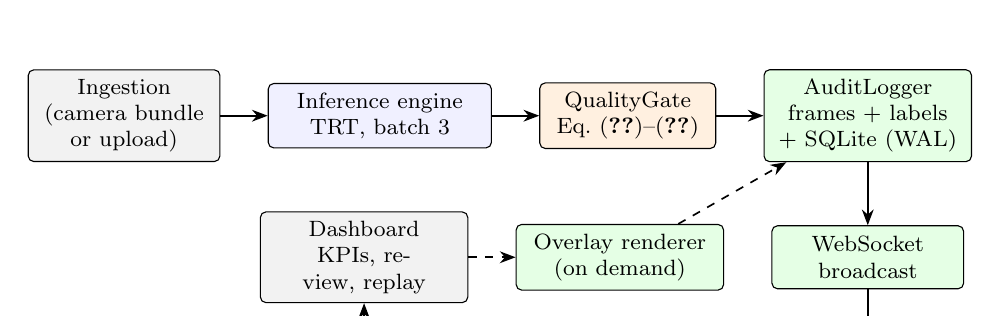
\begin{tikzpicture}[node distance=6mm, every node/.style={font=\footnotesize}]
\node[data, text width=2.2cm] (ing) {Ingestion\\(camera bundle\\or upload)};
\node[stage, text width=2.6cm, right=of ing] (inf) {Inference engine\\TRT, batch 3};
\node[dec, text width=2.0cm, right=of inf] (qg) {QualityGate\\Eq.~\eqref{eq:gate}--\eqref{eq:agg}};
\node[res, text width=2.4cm, right=of qg] (aud) {AuditLogger\\frames + labels\\+ SQLite (WAL)};
\node[res, text width=2.2cm, below=8mm of aud] (ws) {WebSocket\\broadcast};
\node[res, text width=2.4cm, left=of ws] (vis) {Overlay renderer\\(on demand)};
\node[blk, fill=gray!10, text width=2.4cm, left=of vis] (ui) {Dashboard\\KPIs, review, replay};
\foreach \a/\b in {ing/inf,inf/qg,qg/aud,aud/ws} \draw[arr] (\a) -- (\b);
% live stream runs below the renderer so it does not cross it
\draw[arr] (ws.south) -- ++(0,-5mm) -| (ui.south);
\draw[arr, dashed] (ui) -- (vis); \draw[arr, dashed] (vis) -- (aud);
\end{tikzpicture}
\end{adjustbox}
\caption[Integration flow for one Station 1 inspection]{Integration flow for one Station 1 inspection. Solid arrows: per-inspection path; dashed: on-demand overlay requests from the dashboard.}
\label{fig:integration-flow}
\end{figure}

\subsection{Services, concurrency, and GPU memory}
Each station is owned by a singleton service (\texttt{PipelineService}, \texttt{FillPipelineService}) that holds the engine, gate, logger, and renderer. Inference never runs on the server's event loop: asynchronous routes hand work to a thread pool. One TensorRT execution context is not thread-safe, so each service serialises inspections with an inference lock; loading and unloading an engine is guarded by a separate engine lock, and the two are always taken in the order inference lock, then engine lock, which rules out deadlock. Because a station switch can unload the engine at any moment, the code reads the engine reference once into a local variable before using it. On a switch the dashboard calls \texttt{POST /api/unload} and then \texttt{POST /api/fill/load} (or the reverse), so only one station's engines occupy GPU memory.

\subsection{Audit trail}
Station 1 writes one row per bottle to an \texttt{inspections} table (bottle identifier, timestamp, verdict, actuator flag, primary defect and confidence, flagged cameras, decision reason, latency, camera count, path of the stored bundle) and one row per defect to a \texttt{defect\_events} table, with indices on identifier, verdict, time, and defect. Station 2 writes a \texttt{fill\_inspections} table that adds the fill status, ratio, meniscus height, bottle height, and both detector confidences. Both databases run SQLite in write-ahead-log mode. Each bundle directory stores the raw frames and YOLO-format labels, so stored inspections can be exported directly as training data.

\subsection{Operator dashboard (O5)}
\label{sec:dashboard}
The dashboard is a React application served by nginx. A station context holds the active station and swaps the WebSocket stream, the API endpoints, and the page set. Table~\ref{tab:dashboard} lists what is implemented.

\begin{table}[htbp]
\centering
\caption{Operator dashboard features}
\label{tab:dashboard}
\begin{tabularx}{\textwidth}{|L{3.2cm}|X|}
\hline
\textbf{Feature} & \textbf{Implementation} \\ \hline
Live view & Station 1: three-camera feed with per-view overlays and a conveyor filmstrip of recent bottles; Station 2: single feed with the fill-ratio ruler. Driven by the WebSocket stream. \\ \hline
KPI bar & Total inspected, compliance yield, rejection rate, and latest or average cycle latency. The throughput tile is currently estimated from the inspection count; the measured line rate comes from the stress test (Table~\ref{tab:stress}). \\ \hline
Analytics & Defect-class breakdown (Station 1) and fill-ratio histogram (Station 2). \\ \hline
Audit page & Searchable, filterable, paginated history of all inspections with latency per record; CSV export (RFC 4180) for both stations. \\ \hline
Replay inspector & Re-opens any stored bottle with mask blending, per-view contours, decision reason, and navigation to adjacent bottles. \\ \hline
Review queue & \texttt{UNCERTAIN} products are listed for review; the operator corrects polygons or labels and exports the reviewed set as a YOLO dataset (active learning). \\ \hline
Settings & Per-station gate thresholds ($\tau_p,\tau_d,\tau_u$; $\theta_u,\theta_o$) editable at run time. \\ \hline
Camera input & The ingestion layer has a threaded \texttt{VideoCapture} worker for USB and RTSP sources that keeps only the latest frame; the evaluation used uploads and the simulation feed, and live-camera operation was not tested. \\ \hline
Not implemented & Automated PDF shift report and a latency histogram view (listed as future work). \\ \hline
\end{tabularx}
\end{table}

Figures~\ref{fig:dash-cap}--\ref{fig:dash-label} show the operator interface of each station after one simulated inspection. The two station dashboards were captured from the standalone deployment (\texttt{start\_standalone.bat}) on a development machine without a CUDA GPU, so the hardware badge reads ``CPU Fallback'' and the latency tiles show CPU times, not the TensorRT times of Chapter~\ref{ch:results}.

\begin{figure}[htbp]
\centering
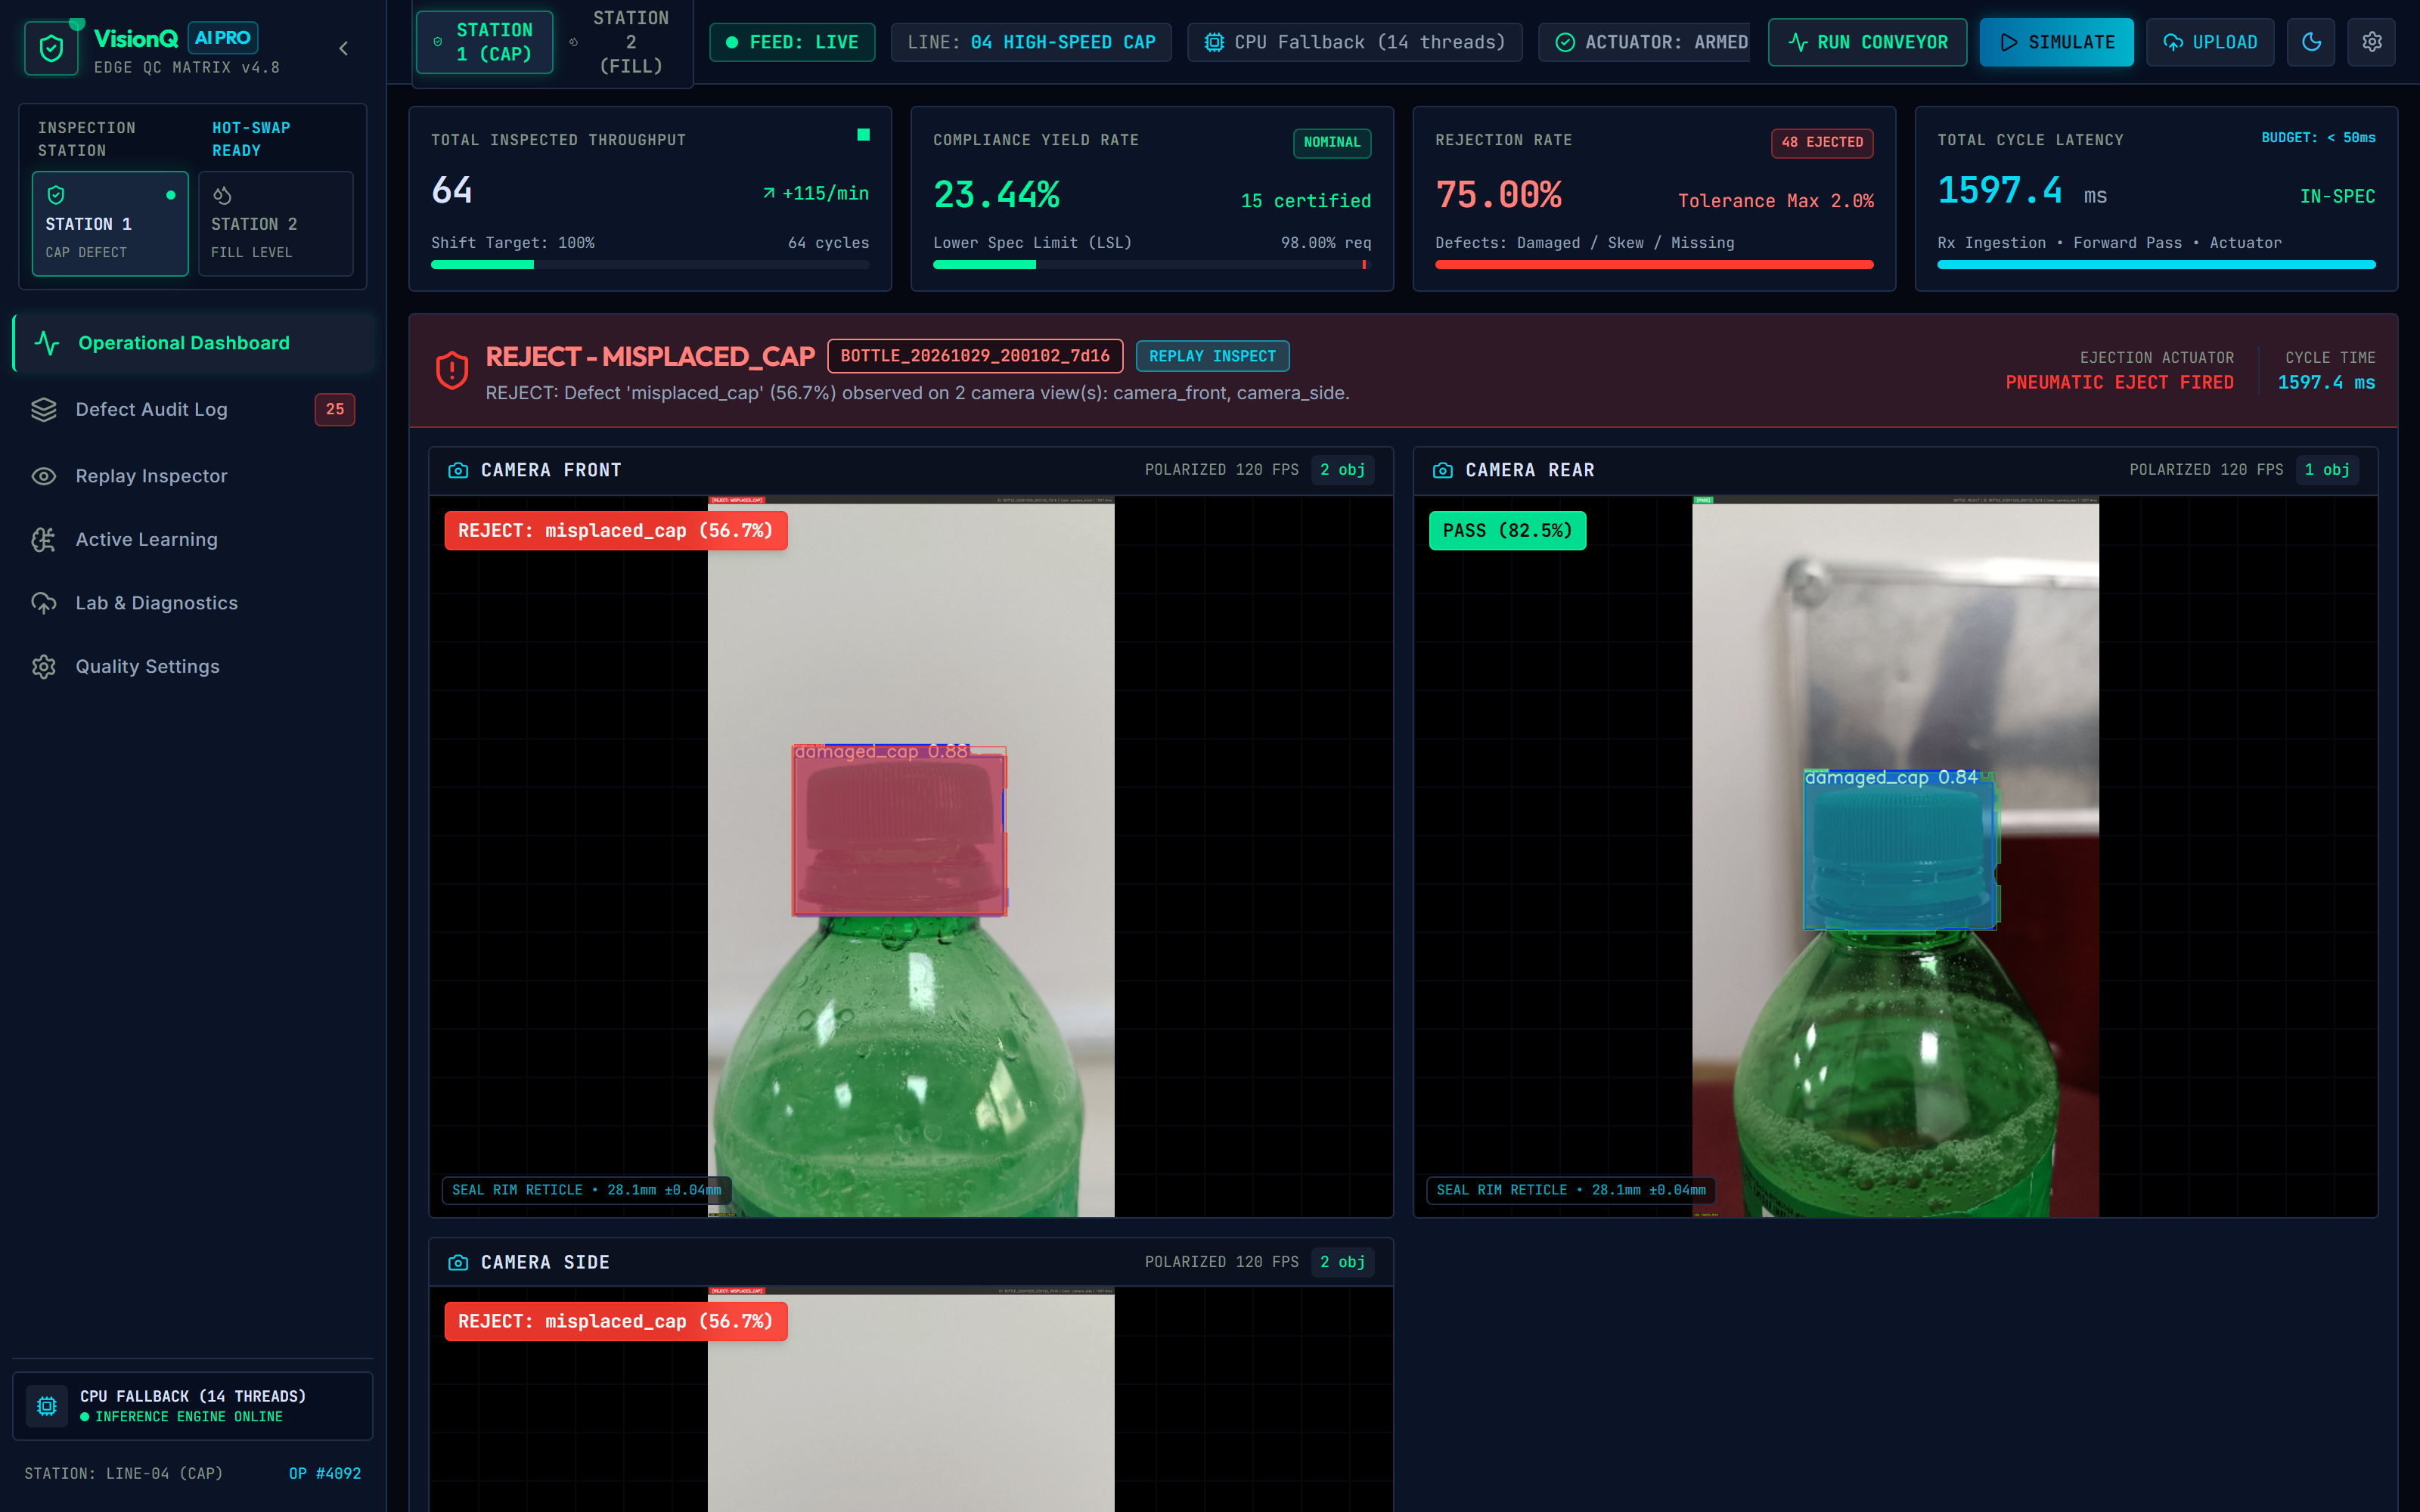
\includegraphics[width=\textwidth]{figures/dashboard_cap.png}
\caption[Station 1 (cap) dashboard after one simulated inspection]{Station 1 (cap) dashboard after one simulated inspection. The banner gives the bottle verdict (\texttt{REJECT}, misplaced cap on two of three views) and fires the reject actuator; each camera panel shows its own per-view verdict, mask overlay, and detection count.}
\label{fig:dash-cap}
\end{figure}

\begin{figure}[htbp]
\centering
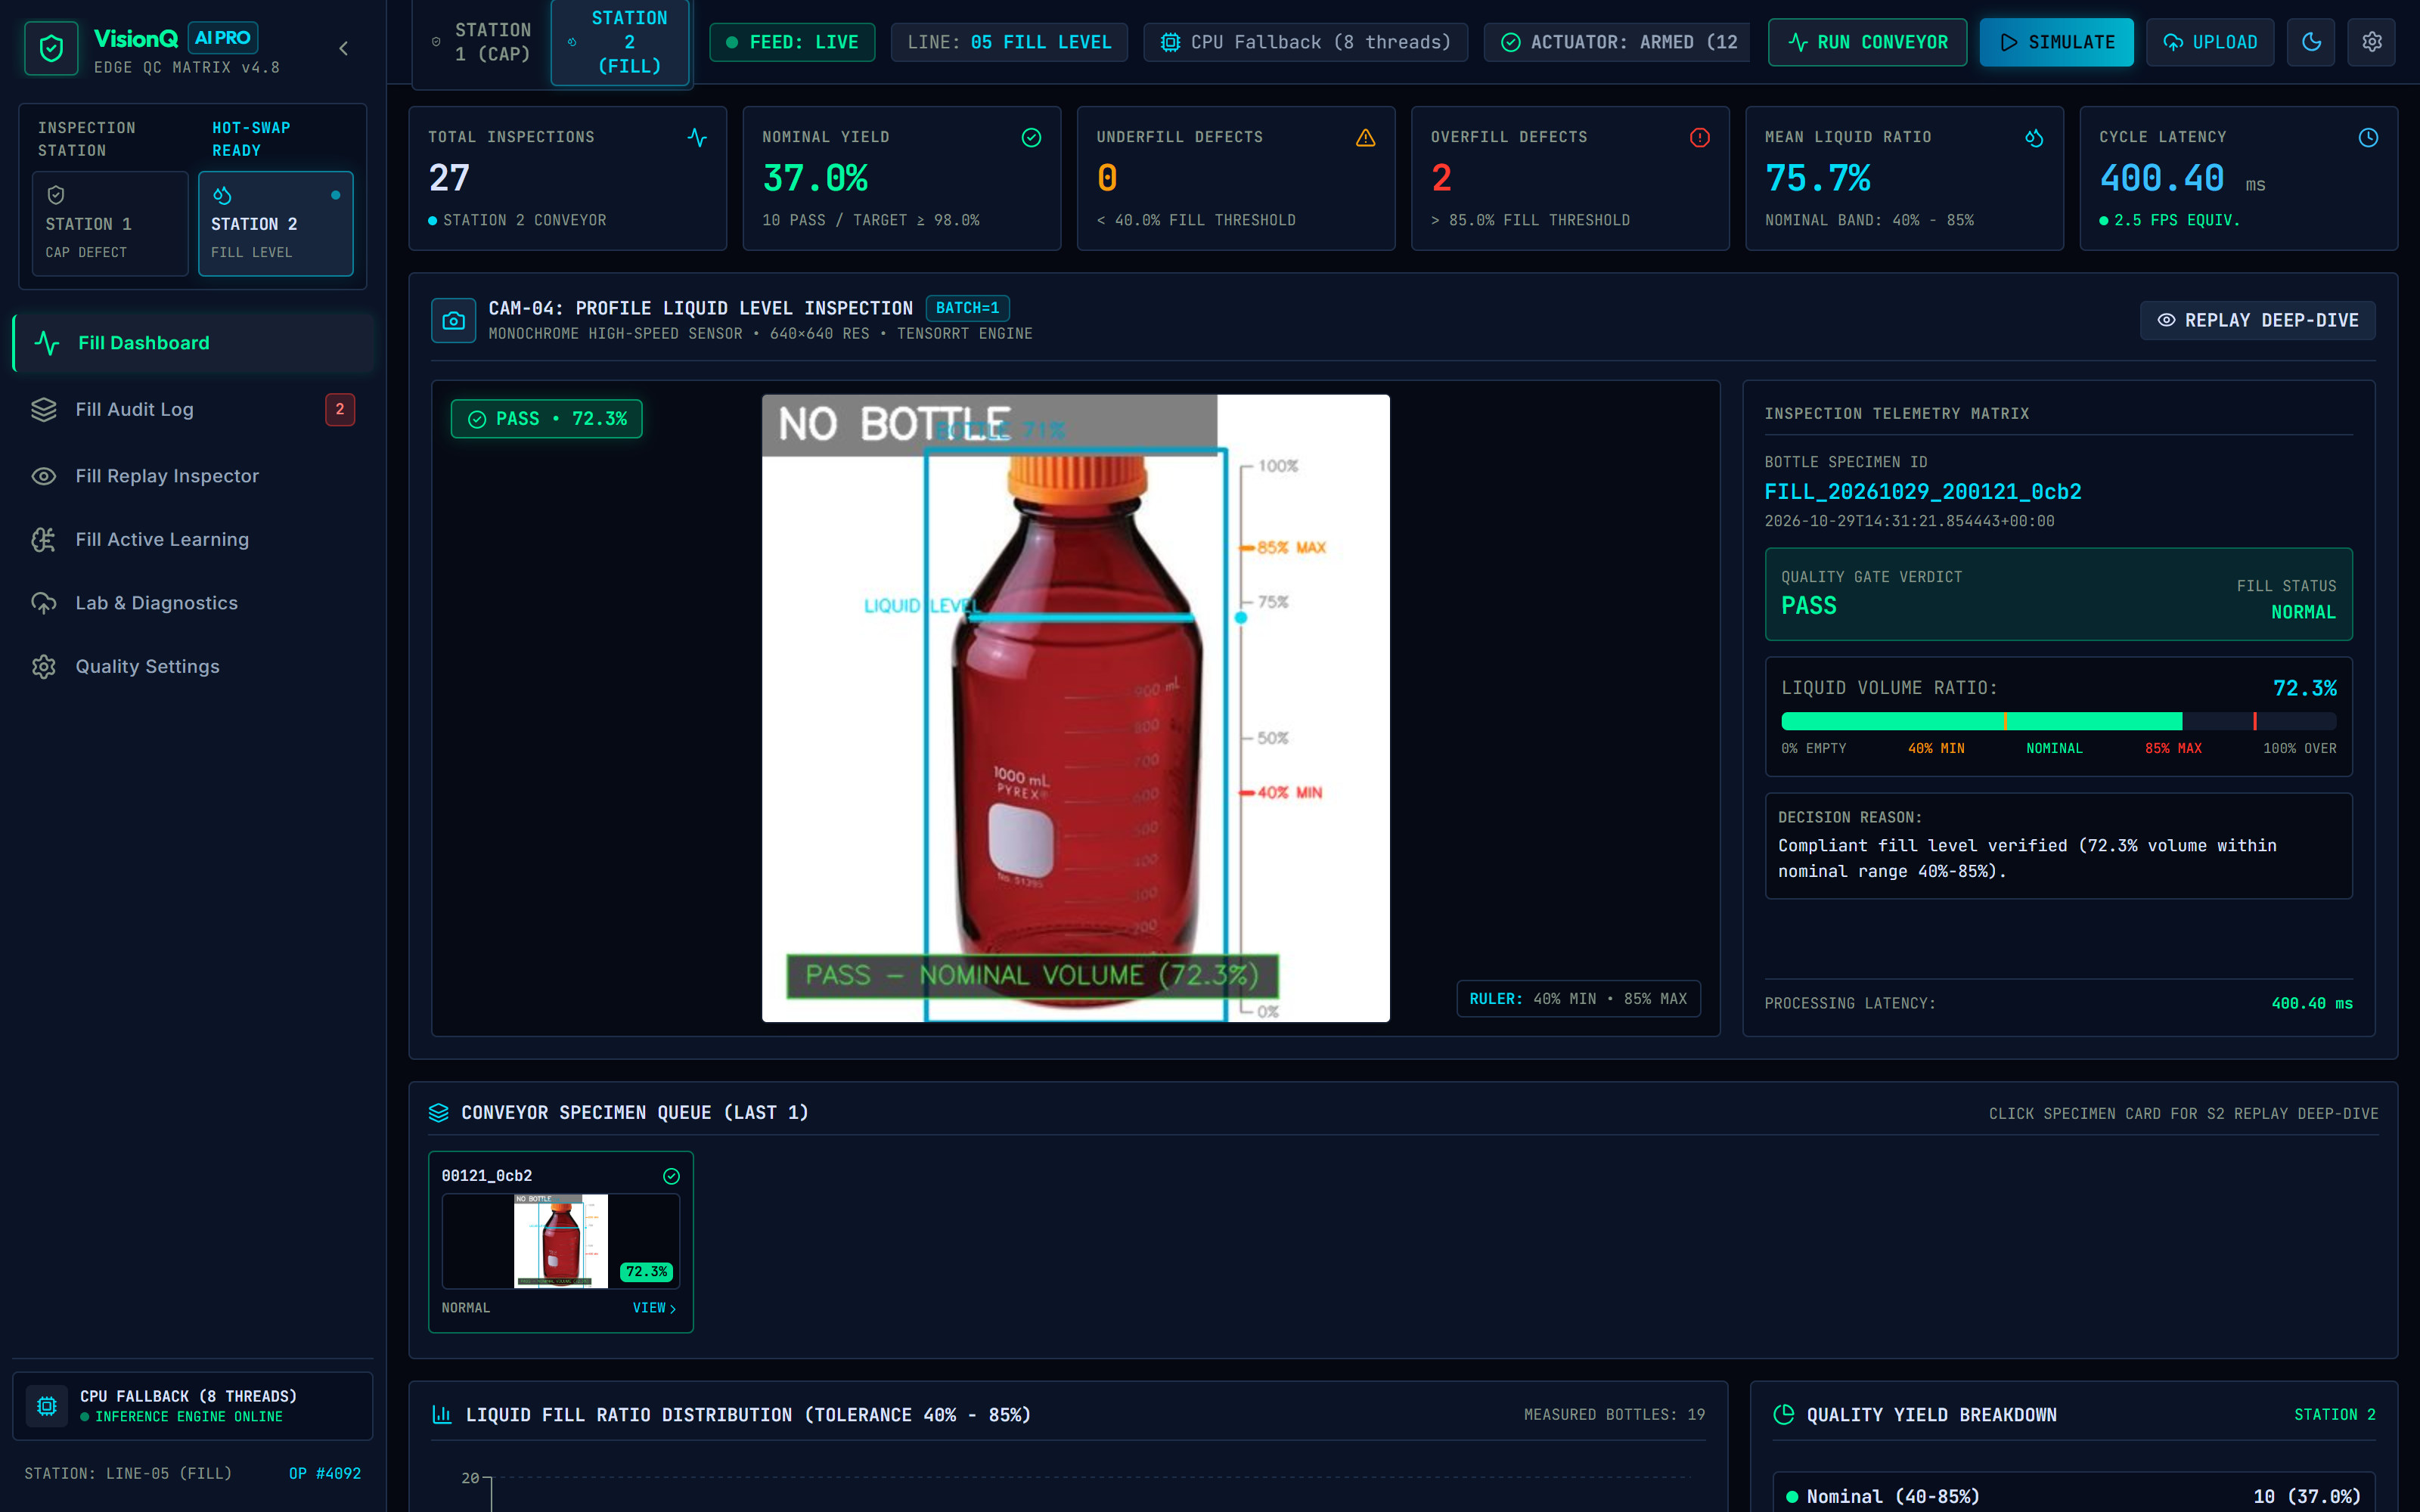
\includegraphics[width=\textwidth]{figures/dashboard_fill.png}
\caption[Station 2 (fill level) dashboard after one simulated inspection]{Station 2 (fill-level) dashboard after one simulated inspection. The frame shows the bottle box, the meniscus line, and the ruler with the 40\% and 85\% limits; the telemetry panel gives the fill ratio (72.3\%), the gate verdict (\texttt{PASS}), and the decision reason. The text banner at the top of the frame is part of the stored sample image.}
\label{fig:dash-fill}
\end{figure}

\begin{figure}[htbp]
\centering
\IfFileExists{figures/dashboard_label.png}{%
  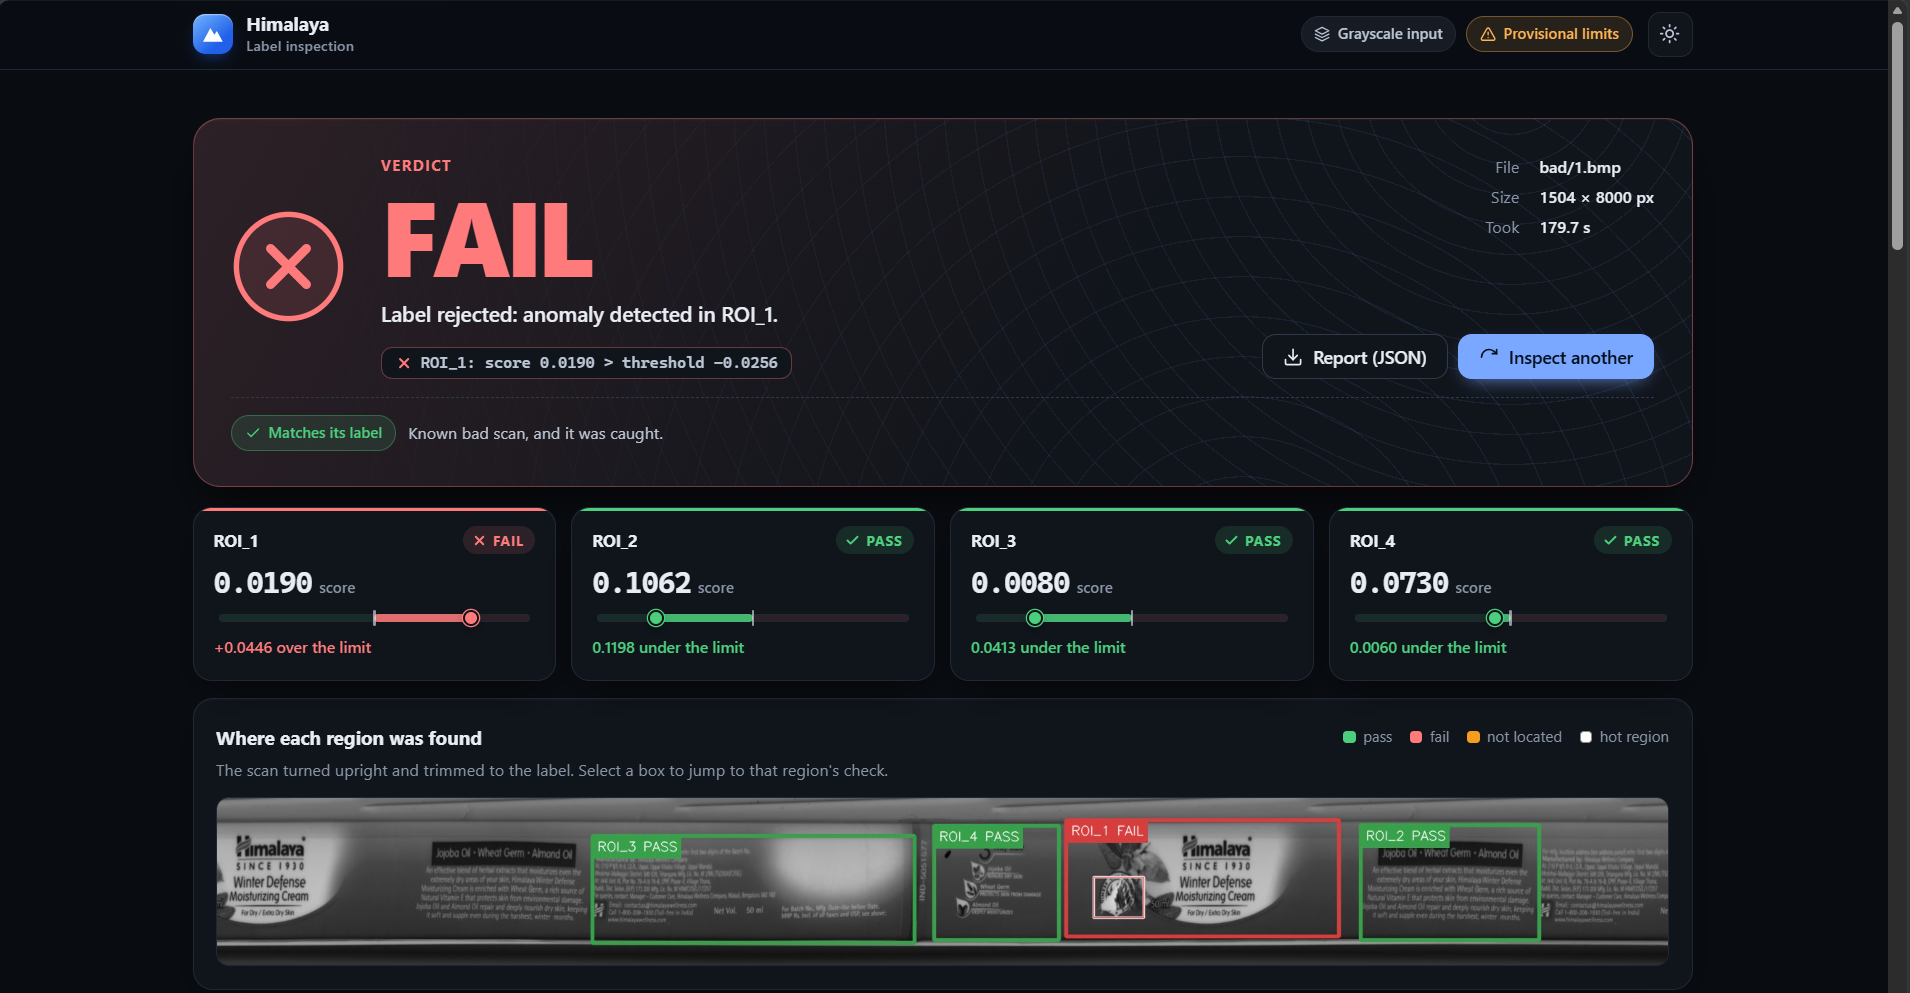
\includegraphics[width=\textwidth]{figures/dashboard_label.png}%
}{%
  \fbox{\parbox[c][6cm][c]{0.9\textwidth}{\centering Placeholder: add \texttt{figures/dashboard\_label.png}\\(label-inspection web application screenshot)}}%
}
\caption[Station 3 (label) inspection application]{Station 3 (label prototype) upload-and-inspect application: label verdict, per-region scores, and anomaly heatmaps for one NSC scan.}
\label{fig:dash-label}
\end{figure}

\subsection{Engine export and deployment}
\label{sec:deploy-impl}
Each PyTorch checkpoint is exported to ONNX and compiled to a TensorRT FP16 engine on the target GPU the first time the station loads. Algorithm~\ref{alg:engine} gives the procedure. The cap engine has a dynamic batch profile (optimum 3, maximum 4), so the three views of a bottle share one execution followed by NMS per view; the two fill engines have a static batch of 1 at 640\,px. Engines are cached under a version tag; changing the tag or setting a force-recompile flag rebuilds them. If no compatible GPU is present, the service falls back to ONNX Runtime and then to PyTorch. All paths come from environment variables resolved against the repository root, so the same code runs natively and in Docker, where the variables point at bind-mounted host folders.

\begin{algorithm}[htbp]
\caption{Engine load with versioned cache and fallback}
\label{alg:engine}
\begin{algorithmic}[1]
\Require Checkpoint path $p$, version tag $v$, batch profile $B$
\Ensure Loaded predictor
\If{CUDA available}
    \State $e \gets$ \texttt{<stem>\_<v>.engine} next to $p$
    \If{$e$ missing \textbf{or} force-recompile set}
        \State export $p \rightarrow$ ONNX $\rightarrow$ TensorRT FP16 with profile $B$ \Comment{minutes on first run}
    \EndIf
    \State load $e$; warm up (two single-image passes, plus a 3-view pass for the cap engine)
    \If{warm-up output shape $\neq$ expected batch} \State rebuild $e$ once \EndIf
\ElsIf{ONNX Runtime installed} \State load \texttt{.onnx}
\Else \State load \texttt{.pt} with PyTorch
\EndIf
\end{algorithmic}
\end{algorithm}

\subsection{Integration challenges}
Table~\ref{tab:challenges} records the main problems met during integration and how they were solved.

\begin{table}[htbp]
\centering
\caption{Integration challenges and solutions}
\label{tab:challenges}
\begin{tabularx}{\textwidth}{|L{4.6cm}|X|}
\hline
\textbf{Challenge} & \textbf{Solution} \\ \hline
TensorRT engine built with static batch 1 silently ran the three views one by one & Dynamic batch profile at export, batched warm-up check, automatic rebuild on shape mismatch. \\ \hline
Engines from one machine fail on another GPU & Compile on the target at first start; cache with version tag. \\ \hline
Two stations' engines in one 24\,GB GPU & Lazy load of Station 2, explicit unload/load on switch, inference and engine locks. \\ \hline
Inference blocking the web server & Thread-pool execution of all inference calls. \\ \hline
Host paths differ between machines and Docker & Environment-driven paths resolved against the repository root; Compose maps host folders to fixed container paths. \\ \hline
Label models fed the wrong colour mode & Threshold files record the input mode and score statistic; the CLI and web app refuse mismatched settings. \\ \hline
\end{tabularx}
\end{table}

\section{Software Testing}
\label{sec:testing-validation}

Testing followed the layer structure. Each station has one test script per layer (ingestion, inference, gate, audit, visualiser, API), an in-process end-to-end test runs both stations and the station swap, a stress test drives the full Station 1 loop inside the container, and the label prototype has 30 model-free unit tests for localisation, explainability, and the web app. Model accuracy was validated on held-out test splits that were not used for training or model selection (Chapter~\ref{ch:results}). Table~\ref{tab:test-results} lists representative test cases, including the failures.

\begin{table}[htbp]
\centering
\caption{Representative test cases}
\label{tab:test-results}
\begin{tabularx}{\textwidth}{|L{3.4cm}|L{3.2cm}|L{2.8cm}|X|}
\hline
\textbf{Test case} & \textbf{Input} & \textbf{Expected} & \textbf{Actual} \\ \hline
Cap gate, held-out test & 354 test images, FP16 engine & FAR $\leq3\%$, FRR $\leq7\%$ & 0/153 and 0/201 (Passed) \\ \hline
FP16 vs FP32 accuracy & Test split & $|\Delta\mAP|<0.01$ & $\leq0.0013$ overall (Passed) \\ \hline
Station swap & Cap$\rightarrow$fill$\rightarrow$cap in one process & Engines released and reloaded & Passed (in-process, CPU/ONNX) \\ \hline
Fill verdict agreement & 41 meniscus test images & $\geq0.93$ & 34/35 = 0.971 (Passed) \\ \hline
Fill, multi-bottle rack frames & 4 rack frames & Graceful handling & No bottle found $\Rightarrow$ \texttt{INSPECTION\_FAILED} (by design) \\ \hline
Closed loop at 300 bottles/min & 500 unpaced cycles & p50 $\leq200$\,ms & 299\,ms (Failed: storage-bound) \\ \hline
Paced run, 150 bottles/min & 300 cycles & 150 bottles/min & 126.7 bottles/min (Failed) \\ \hline
Database integrity under load & 800 cycles in total & No failed writes & 0 failures (Passed) \\ \hline
Label localisation & 120 NSC scans & All 4 ROIs found & 480/480 (Passed) \\ \hline
Label overlap rule & 120 NSC scans & No false re-assignment & Rule never fired (Passed) \\ \hline
Label ROI\_4 precision & 35 held-out crops & High precision & 57.9\% (Open issue) \\ \hline
\end{tabularx}
\end{table}

%======================================================================
\chapter{Results and Discussion}
\label{ch:results}

This chapter reports the measured results of every station, compares them with the Phase 1 approach and with the targets set in Chapter~\ref{ch:intro}, and discusses what they do and do not show. The setup, metrics, and baselines are defined in Section~\ref{sec:setup}. Unless stated otherwise, accuracy figures are on held-out test splits that were not used for training, model selection, or threshold setting.

\section{Experimental Results}
\label{sec:experimental-results}

\subsection{Cap dataset and artefacts (O1)}
\label{sec:res-o1}
Table~\ref{tab:capdata} gives the per-class counts found on disk. The Roboflow export notes 8,530 images, but the three splits contain 8,524. Every image shows one bottle neck with one annotated cap, captured at $2048{\times}2048$ (a handful at $2048{\times}1536$) against indoor backgrounds. The training split holds 2,486 source photographs, each exported in three augmented versions (rotation $\pm5^\circ$, brightness $\pm25\%$, blur up to 2\,px, 0.5\% salt-and-pepper noise); validation and test images are not augmented. The masks come from a single annotator, so inter-annotator agreement cannot be measured.

\begin{table}[htbp]
\centering
\caption{Six-class cap dataset (one cap per image)}
\label{tab:capdata}
\begin{tabular}{|l|r|r|r|r|}
\hline
\textbf{Class} & \textbf{Train} & \textbf{Valid} & \textbf{Test} & \textbf{Share of train} \\ \hline
good\_cap & 4,242 & 405 & 201 & 56.9\% \\ \hline
wet\_cap & 828 & 79 & 39 & 11.1\% \\ \hline
open\_cap & 768 & 65 & 38 & 10.3\% \\ \hline
damaged\_cap & 648 & 62 & 31 & 8.7\% \\ \hline
no\_cap & 645 & 61 & 30 & 8.6\% \\ \hline
misplaced\_cap & 327 & 40 & 15 & 4.4\% \\ \hline
\textbf{Total images} & \textbf{7,458} & \textbf{712} & \textbf{354} & \\ \hline
Source photographs & 2,486 & 712 & 354 & \\ \hline
\end{tabular}
\end{table}

The cap is not a small object in this dataset: its median bounding box covers 9.2\% of the test image (10th--90th percentile 6.0--14.0\%), and after resizing to the 640-pixel network input every instance is ``large'' by the COCO definition ($\geq96^2$ pixels)~\cite{lin2014coco}. What is small is the evidence inside the cap: droplets on wet caps, dents on damaged caps, and the thread gap of open caps. ``Small-object-aware'' in the primary objective therefore refers to preserving fine intra-object detail, which is what the distillation sites target, rather than detecting tiny objects.

Table~\ref{tab:artefacts} lists the exported artefacts of the cap model. The FP16 engine is about half the size of the FP32 ONNX graph, and Section~\ref{sec:res-seg} shows that it keeps the model's accuracy. As the benchmark for future model versions, a held-out test grouped by capture session has been identified, so that images of the same session never appear in both training and test.

\begin{table}[htbp]
\centering
\caption{Cap model artefacts}
\label{tab:artefacts}
\begin{adjustbox}{max width=\textwidth}
\begin{tabular}{|l|l|r|l|}
\hline
\textbf{Artefact} & \textbf{Precision} & \textbf{Size (MB)} & \textbf{Use} \\ \hline
PyTorch checkpoint (\texttt{best.pt}) & FP32 & 45.2 & Training, PyTorch fallback \\ \hline
ONNX graph & FP32 & 90.5 & Portable runtime, TensorRT input \\ \hline
TensorRT engine (\texttt{best\_v1.engine}) & FP16, dynamic batch & 49.1 & Deployment on the target GPU \\ \hline
\end{tabular}
\end{adjustbox}
\end{table}

\subsection{Distillation outcome}
\label{sec:res-kd}
Table~\ref{tab:kd} compares teacher and student, both evaluated in FP32 with the same Ultralytics validation on the same splits. Figure~\ref{fig:curve} shows the student's validation mAP during distillation training.

\begin{table}[htbp]
\centering
\caption{Teacher versus distilled student (FP32, 640\,px)}
\label{tab:kd}
\begin{tabular}{|l|c|c|}
\hline
 & \textbf{Teacher YOLO11x-seg} & \textbf{Student YOLO11m-seg} \\ \hline
Parameters (M) & 62.06 & 22.34 \\ \hline
GFLOPs @640 & 297.4 & 113.0 \\ \hline
Checkpoint size (MB) & 124.8 & 45.2 \\ \hline
Inference per image (ms)$^{*}$ & 19.0 & 7.8 \\ \hline
\multicolumn{3}{|l|}{\textit{Test split ($n=354$)}} \\ \hline
Box precision / recall & 0.995 / 0.997 & 0.998 / \textbf{1.000} \\ \hline
Box / mask mAP@0.5 & 0.995 / 0.995 & 0.995 / 0.995 \\ \hline
Box mAP@0.5:0.95 & \textbf{0.944} & 0.927 \\ \hline
Mask mAP@0.5:0.95 & 0.912 & \textbf{0.927} \\ \hline
\multicolumn{3}{|l|}{\textit{Per-class mask mAP@0.5:0.95 (test)}} \\ \hline
damaged / good & 0.929 / 0.877 & 0.927 / \textbf{0.893} \\ \hline
misplaced / no cap & 0.899 / 0.913 & \textbf{0.941} / 0.915 \\ \hline
open / wet & 0.931 / 0.924 & 0.935 / \textbf{0.953} \\ \hline
\multicolumn{3}{|l|}{\textit{Validation split ($n=712$)}} \\ \hline
Box / mask mAP@0.5:0.95 & 0.946 / 0.913 & 0.938 / \textbf{0.936} \\ \hline
\multicolumn{3}{l}{\small $^{*}$PyTorch FP32, batch 1, Ultralytics validation; teacher timed on its training GPU.}
\end{tabular}
\end{table}

The student matches the teacher's mAP@0.5 of 0.995 on every class with 2.8$\times$ fewer parameters, 2.6$\times$ fewer FLOPs, and a 2.8$\times$ smaller checkpoint, and it runs 2.4$\times$ faster per image. At strict IoU the two models trade places. The student's \emph{mask} mAP@0.5:0.95 is higher than the teacher's on both test (0.927 vs.\ 0.912) and validation (0.936 vs.\ 0.913), and higher for five of six classes, with damaged caps level (0.927 vs.\ 0.929). The gain is largest on the classes whose evidence is finest: wet (+0.029), misplaced (+0.042), and good (+0.016). The teacher keeps a lead in \emph{box} mAP@0.5:0.95 (0.944 vs.\ 0.927). Station 1 decides from the cap's region and stores its mask, so the mask trade is the one the application favours. The student also has higher test recall (1.000 vs.\ 0.997; the teacher misses one open cap) and makes no spurious background detection, where the teacher makes one.

\begin{figure}[htbp]
\centering
\begin{tikzpicture}
\begin{axis}[width=0.85\textwidth, height=6cm, xlabel={epoch}, ylabel={validation mAP@0.5:0.95}, ymin=0.4, ymax=1.0, xmin=0, xmax=127, legend pos=south east, legend style={font=\footnotesize}, grid=major, grid style={gray!20}]
\addplot[blue, thick] table[x=epoch, y=maskmap] {figures/student_curve.dat};
\addplot[red, dashed] table[x=epoch, y=boxmap] {figures/student_curve.dat};
\draw[gray, dashed] (axis cs:96,0.4) -- (axis cs:96,1.0);
\node[gray, font=\footnotesize, anchor=south east] at (axis cs:95,0.42) {best epoch 96};
\legend{mask, box}
\end{axis}
\end{tikzpicture}
\caption[Student validation mAP during distillation training]{Validation mAP@0.5:0.95 of the YOLO11m-seg student during distillation training. Training stopped early at epoch 126 (patience 30).}
\label{fig:curve}
\end{figure}

Figure~\ref{fig:prcm} shows the student's mask precision--recall curves and normalised confusion matrix on the validation split. Every class reaches AP@0.5 of 0.995; the only off-diagonal mass is a small confusion between misplaced and open caps.

\begin{figure}[htbp]
\centering
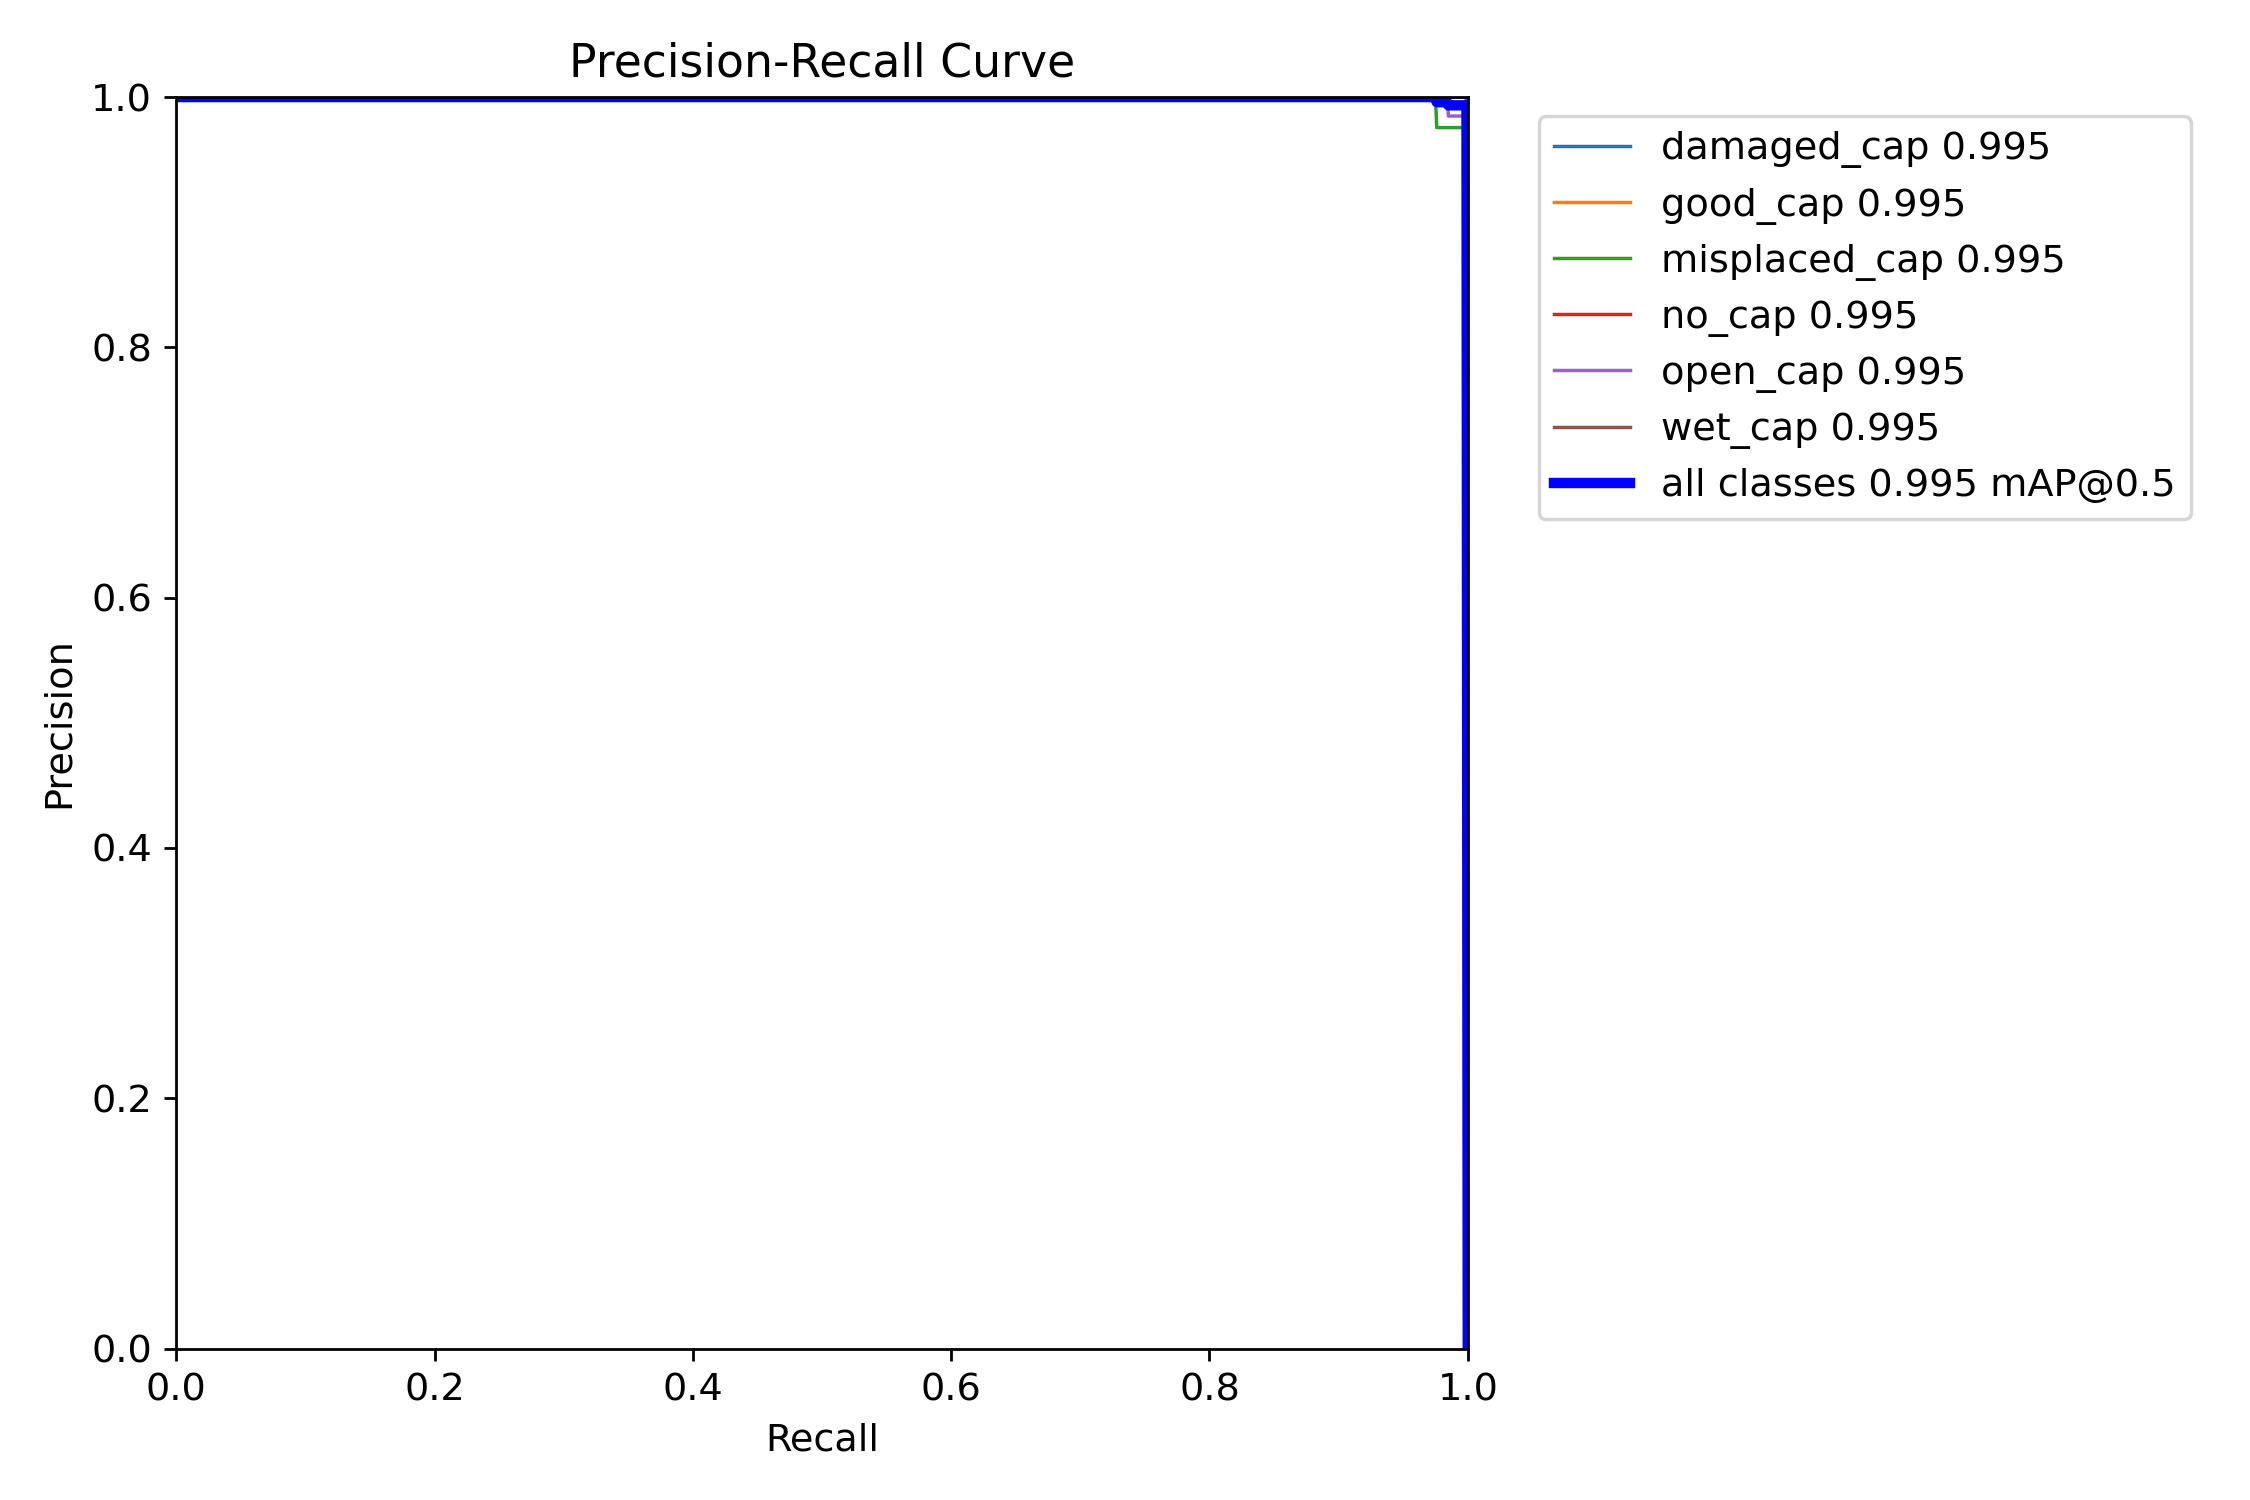
\includegraphics[width=0.49\textwidth]{figures/student_maskpr.png}\hfill
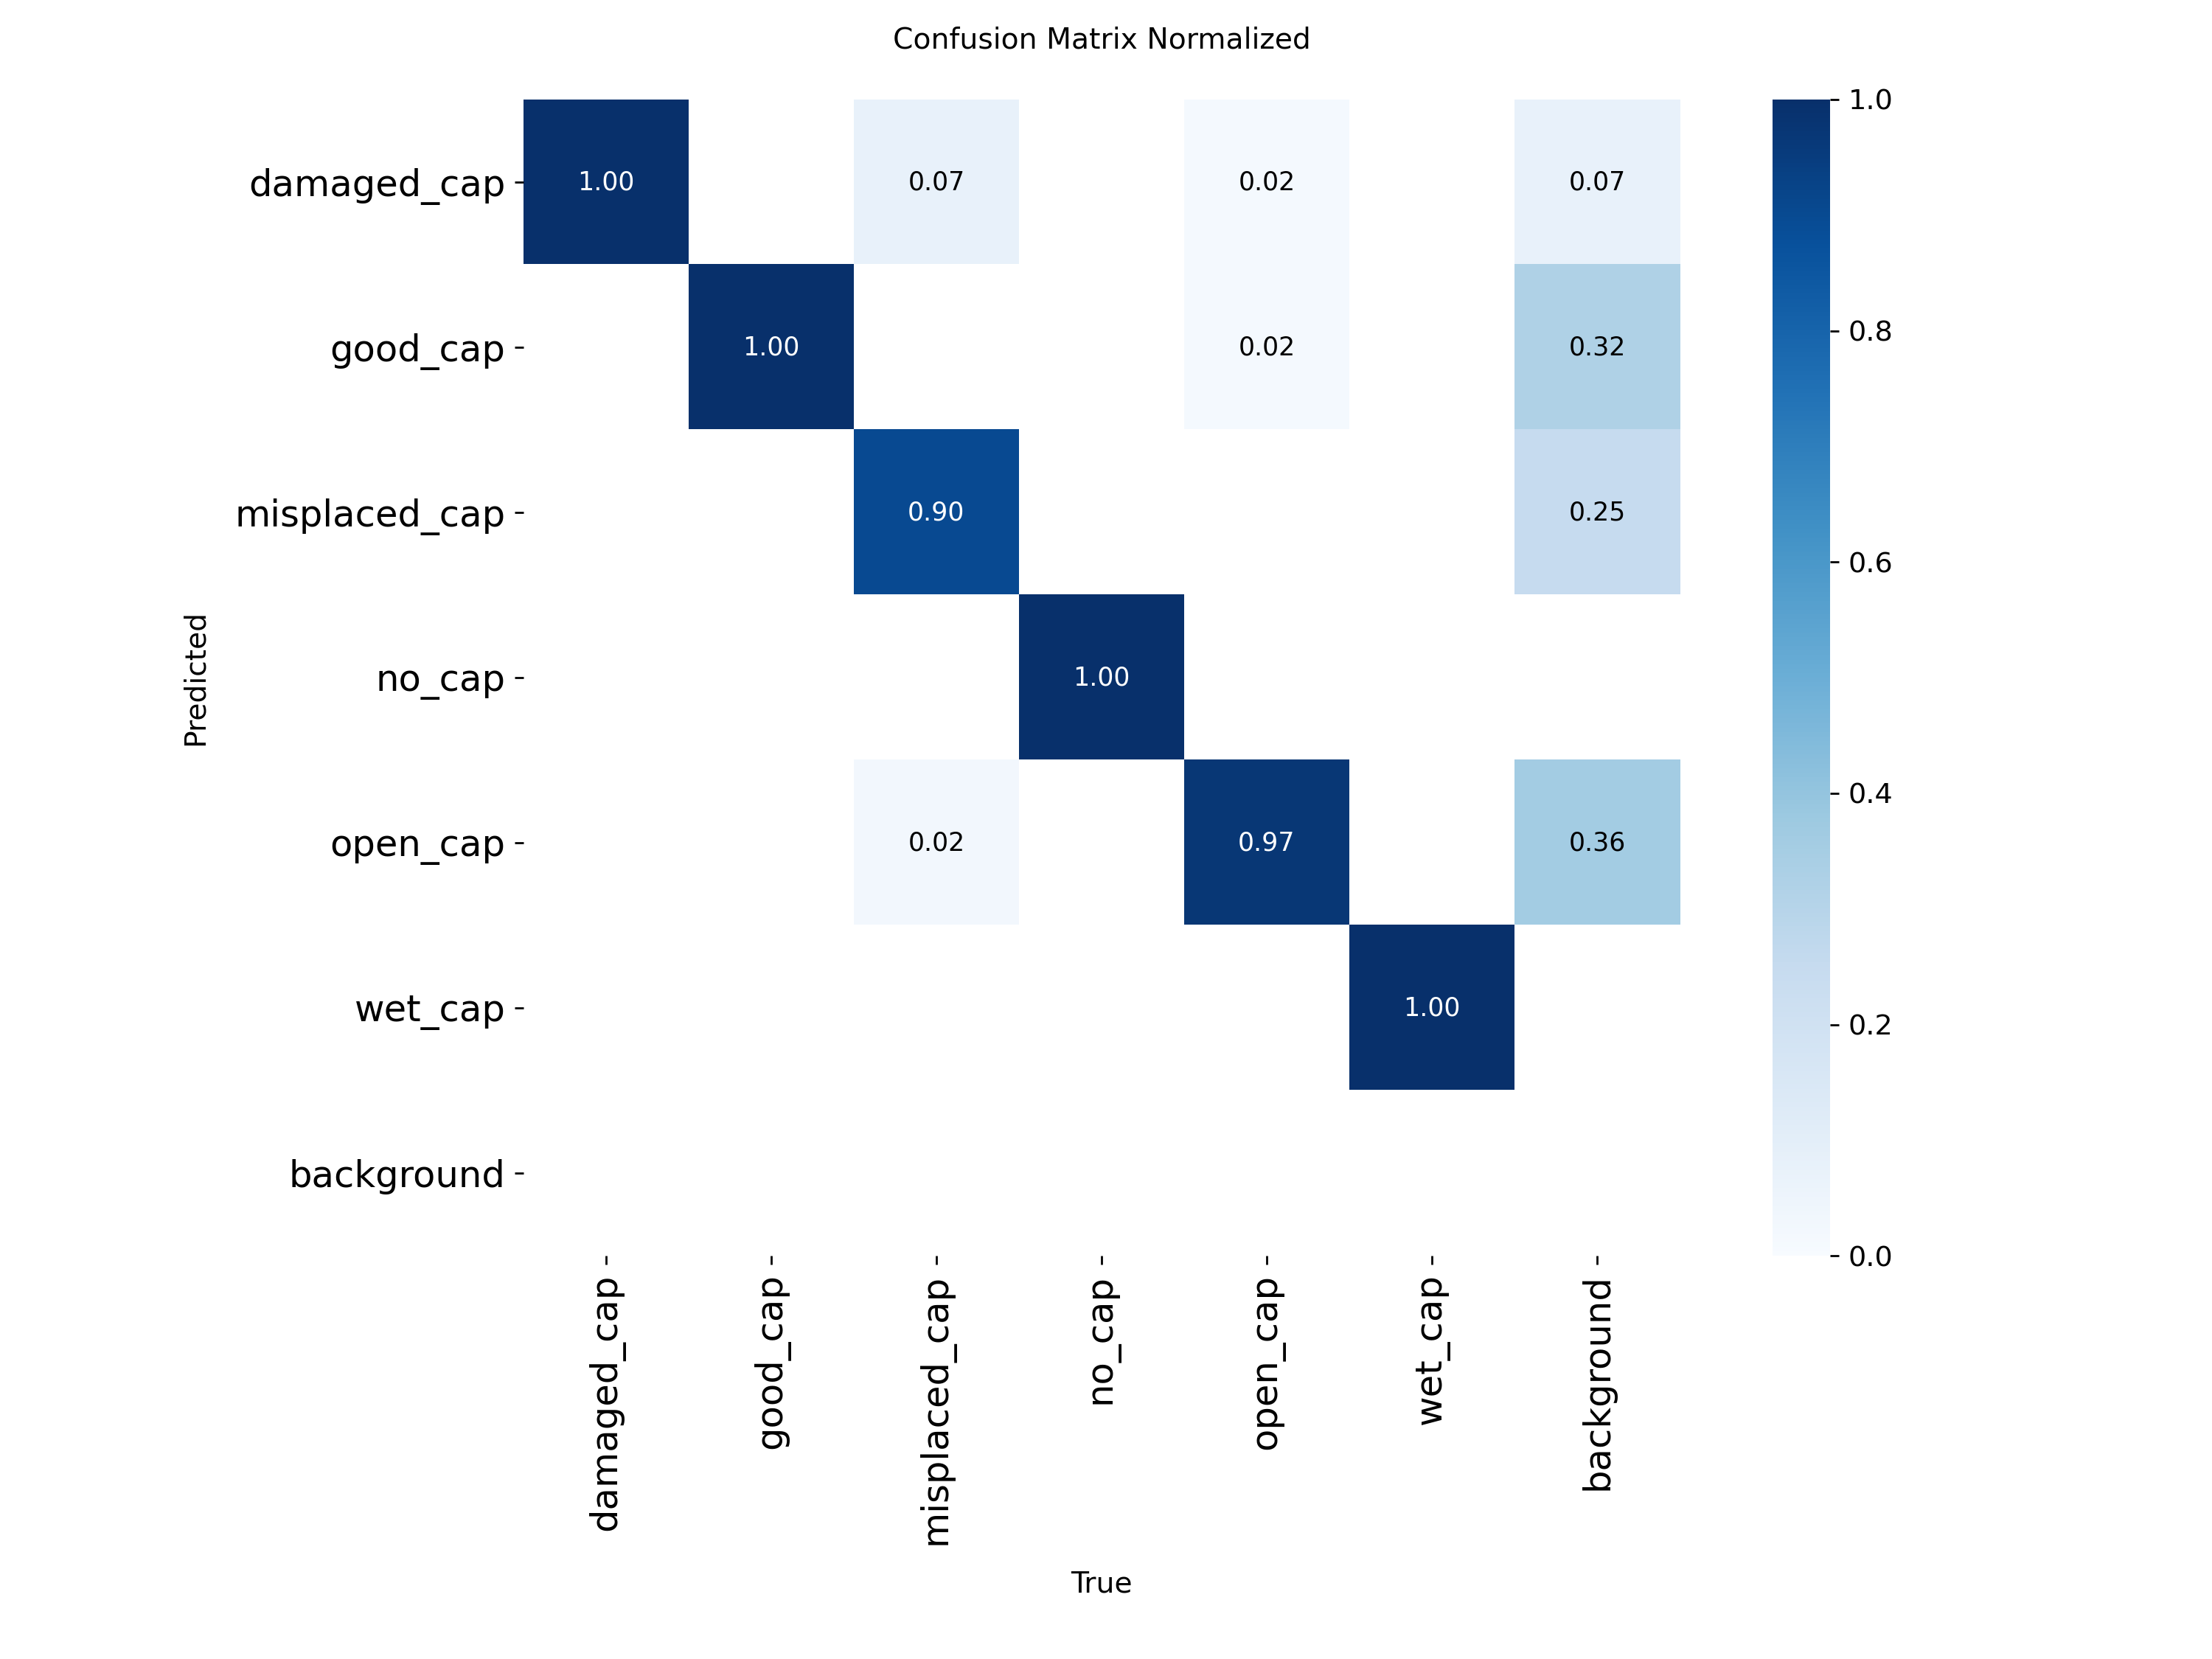
\includegraphics[width=0.49\textwidth]{figures/student_confusion.png}
\caption[Student precision--recall curves and confusion matrix]{Student YOLO11m-seg on the validation split: (left) mask precision--recall curves per class; (right) normalised confusion matrix.}
\label{fig:prcm}
\end{figure}

\subsection{Cap segmentation: trained versus deployed model}
\label{sec:res-seg}
Table~\ref{tab:seg} reports per-class segmentation metrics for the FP32 checkpoint and the deployed FP16 engine. Both reach AP@0.5 of 0.995 for every class. Converting to FP16 changes overall mAP@0.5:0.95 by at most 0.0013 and any single class by at most 0.006. The lowest strict-IoU score is for good-cap masks (0.893), where the boundary against the bottle neck is least distinct.

\begin{table}[htbp]
\centering
\caption{Station 1 segmentation on the held-out test split ($n=354$)}
\label{tab:seg}
\begin{tabular}{|l|c|c|c|c|}
\hline
 & \multicolumn{2}{c|}{\textbf{FP32 PyTorch}} & \multicolumn{2}{c|}{\textbf{FP16 TensorRT}} \\ \hline
\textbf{Class (support)} & \textbf{Mask AP$_{50:95}$} & \textbf{Box AP$_{50:95}$} & \textbf{Mask} & \textbf{Box} \\ \hline
damaged (31) & 0.927 & 0.952 & 0.931 & 0.958 \\ \hline
good (201) & 0.893 & 0.904 & 0.894 & 0.903 \\ \hline
misplaced (15) & 0.941 & 0.930 & 0.942 & 0.930 \\ \hline
no cap (30) & 0.915 & 0.922 & 0.915 & 0.922 \\ \hline
open (38) & 0.935 & 0.928 & 0.933 & 0.929 \\ \hline
wet (39) & 0.953 & 0.929 & 0.953 & 0.930 \\ \hline
\textbf{All: mAP$_{50:95}$} & 0.927 & 0.927 & 0.928 & 0.929 \\ \hline
All: P / R & \multicolumn{2}{c|}{0.998 / 1.000} & \multicolumn{2}{c|}{0.998 / 1.000} \\ \hline
Valid: mAP$_{50:95}$ & 0.936 & 0.938 & 0.936 & 0.937 \\ \hline
\end{tabular}
\end{table}

Taking the highest-scoring detection above the 0.35 floor as the image label, top-1 classification is correct for 354 of 354 test images and 710 of 712 validation images (macro-F1 0.993, Cohen's $\kappa$ 0.996, MCC 0.996). Both validation errors are misplaced caps predicted as open caps; both are defect classes, so the bottle verdict is still \texttt{REJECT}.

\subsection{Product-level error and threshold analysis}
\label{sec:res-gate}
Table~\ref{tab:gate} replays the production gate image by image with the deployed engine. Each image counts as one bottle seen by one view, because the dataset has no synchronised triplets. No defective cap is passed and no good cap is rejected. With zero observed events, the exact Clopper--Pearson~\cite{clopper1934} 95\% upper bound on a rate with $n$ trials is $1-0.025^{1/n}$, which gives 2.4\% false accept and 1.8\% false reject on the test split.

\begin{table}[htbp]
\centering
\caption{Production gate replayed with the FP16 engine (defaults $\tau_p=0.75$, $\tau_d=0.45$, $\tau_u=0.40$)}
\label{tab:gate}
\begin{tabular}{|l|c|c|}
\hline
 & \textbf{Valid} & \textbf{Test} \\ \hline
PASS / REJECT / UNCERTAIN / FAILED & 405 / 307 / 0 / 0 & 201 / 153 / 0 / 0 \\ \hline
False accept (defect $\rightarrow$ PASS) & 0/307 ($\leq1.2\%$) & 0/153 ($\leq2.4\%$) \\ \hline
False reject (good $\rightarrow$ REJECT) & 0/405 ($\leq0.9\%$) & 0/201 ($\leq1.8\%$) \\ \hline
Auto-decided accuracy & 1.000 & 1.000 \\ \hline
\multicolumn{3}{l}{\small Parentheses: Clopper--Pearson 95\% upper bound.}
\end{tabular}
\end{table}

We swept $\tau_p\in[0.50,0.95]$ and $\tau_d\in[0.25,0.65]$ (Figure~\ref{fig:sweep}). No false accept or false reject occurs at any grid point. The defect threshold has no effect over its whole range, because the engine emits no wrong-polarity score above 0.01 on either split: there is no defect score on good caps and no good-cap score on defective caps. The pass threshold controls only the review load. Good-cap top scores lie in $[0.856, 0.921]$ on test (median 0.897), so review routing starts between $\tau_p=0.85$ and $0.90$; at $0.90$, 34.5\% of test bottles and 36.0\% of validation bottles go to review. The default $\tau_p=0.75$ leaves a margin of $0.106$ below the lowest good-cap score. Defective caps score between 0.820 and 0.941 on test, 0.37 above $\tau_d$. Accuracy is identical across bounding-box-area terciles; the only validation errors fall in the largest tercile.

\begin{figure}[htbp]
\centering
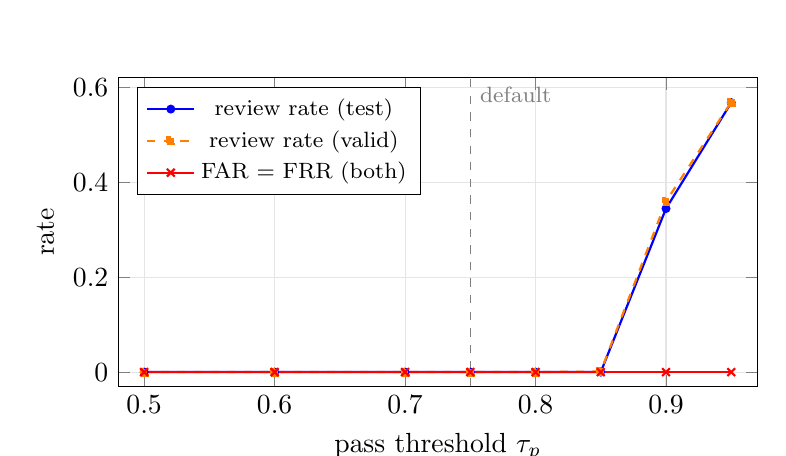
\begin{tikzpicture}
\begin{axis}[width=0.8\textwidth, height=5.5cm, xlabel={pass threshold $\tau_p$}, ylabel={rate}, ymin=-0.03, ymax=0.62, xmin=0.48, xmax=0.97, legend pos=north west, legend style={font=\footnotesize}, grid=major, grid style={gray!20}]
\addplot[blue, thick, mark=*, mark size=1.2pt] coordinates {(0.50,0) (0.60,0) (0.70,0) (0.75,0) (0.80,0) (0.85,0) (0.90,0.3446) (0.95,0.5678)};
\addplot[orange, thick, dashed, mark=square*, mark size=1.2pt] coordinates {(0.50,0) (0.60,0) (0.70,0) (0.75,0) (0.80,0) (0.85,0.0014) (0.90,0.3596) (0.95,0.5688)};
\addplot[red, thick, mark=x] coordinates {(0.50,0) (0.60,0) (0.70,0) (0.75,0) (0.80,0) (0.85,0) (0.90,0) (0.95,0)};
\draw[gray, dashed] (axis cs:0.75,-0.03) -- (axis cs:0.75,0.62) node[below right, font=\footnotesize]{default};
\legend{review rate (test), review rate (valid), FAR $=$ FRR (both)}
\end{axis}
\end{tikzpicture}
\caption[Gate threshold sweep]{Gate threshold sweep with the FP16 engine ($\tau_d=0.45$; every other $\tau_d$ in $[0.25,0.65]$ gives identical curves).}
\label{fig:sweep}
\end{figure}

\subsection{Fill-level estimation (O2)}
\label{sec:res-fill}
Table~\ref{tab:filldet} reports both Station 2 detectors on their held-out test splits at 640\,px. The meniscus detector localises the surface reliably at IoU 0.5 (AP 0.923) but loosely at strict IoU (AP@0.5:0.95 of 0.458). Because Eq.~\eqref{eq:rfill} uses only the box mid-line, this looseness affects the ratio far less than the strict-IoU score suggests. FP16 conversion leaves the meniscus detector unchanged but lowers the bottle detector's AP@0.5:0.95 from 0.578 to 0.481; the deployed bottle engine is built at 640\,px although the detector was trained at 512\,px, and building it at its training resolution is the planned remedy.

\begin{table}[htbp]
\centering
\caption{Station 2 detectors on held-out test splits (640\,px)}
\label{tab:filldet}
\begin{tabular}{|l|l|c|c|c|c|}
\hline
\textbf{Model (class, boxes)} & \textbf{Runtime} & \textbf{P} & \textbf{R} & \textbf{AP$_{50}$} & \textbf{AP$_{50:95}$} \\ \hline
\multirow{2}{*}{YOLOv8s (bottle, 356)} & FP32 & 0.855 & 0.880 & 0.935 & 0.578 \\ \cline{2-6}
 & TRT FP16 & 0.823 & 0.890 & 0.907 & 0.481 \\ \hline
\multirow{2}{*}{YOLOv8n (surface, 76)} & FP32 & 0.904 & 0.867 & 0.923 & 0.458 \\ \cline{2-6}
 & TRT FP16 & 0.883 & 0.882 & 0.921 & 0.459 \\ \hline
\end{tabular}
\end{table}

To isolate the effect of meniscus localisation on the estimate, the deployed engines were run on the 41 surface-test images. For each image the ratio from the predicted surface was compared with the ratio from the annotated surface, using the same predicted bottle box. Table~\ref{tab:fillerr} gives the results. In 31 of 35 evaluable images the ratio differs by at most 0.02, the median difference is 1 pixel (0.002 in ratio), and the fill state agrees in 34 of 35 images. The single disagreement is an overfilled bottle (annotated ratio 0.902) that was passed as acceptable (0.708).

\begin{table}[htbp]
\centering
\caption{Fill-ratio error from meniscus localisation (41 test images, TRT FP16)}
\label{tab:fillerr}
\begin{tabular}{|l|r|}
\hline
No bottle detected (multi-bottle rack frames) & 4 \\ \hline
Bottle found, no surface associated & 2 \\ \hline
Evaluated & 35 \\ \hline
Median $|\Delta R|$ / MAE / 90th percentile / max & 0.002 / 0.023 / 0.022 / 0.300 \\ \hline
$|\Delta R|\leq0.02$ / $\leq0.05$ & 88.6\% / 91.4\% \\ \hline
Fill-state agreement (under / acceptable / over) & 34/35 (97.1\%) \\ \hline
Gate verdicts PASS / REJECT / UNCERTAIN & 27 / 7 / 1 \\ \hline
\end{tabular}
\end{table}

The large errors share one failure mode: when the true surface sits high in the neck, the detector fires on a horizontal structure lower on the body, such as a moulded shoulder rib, a glare band, or the edge of a gripping hand. The two missed surfaces are a tinted bottle held in a hand and a nearly full bottle. All four frames with no bottle detection come from the multi-bottle rack video, which the single-bottle design does not support; they are reported as \texttt{INSPECTION\_FAILED} rather than guessed.

\subsection{Label-defect prototype (O4)}
\label{sec:res-label}

\noindent\textbf{Localisation.} Template matching located all four regions in all 120 NSC scans (480 of 480), taking about 120\,ms per scan on the CPU. The overlap rule never fired, so no region was re-assigned. Localisation therefore needed no labelled boxes and no GPU.

\noindent\textbf{Colour versus grayscale models.} The first EfficientAD models were trained on colour crops. On good crops they flagged large bright areas of the white label background, which produced many false alarms. Retraining on grayscale crops, replicated to three channels, made the models attend to print texture and intensity instead of colour. Table~\ref{tab:label-colour} compares the two for the crop-level evaluation.

\begin{table}[htbp]
\centering
\caption{Label prototype: colour versus grayscale EfficientAD-Medium, crop-level}
\label{tab:label-colour}
\begin{tabular}{|l|r|r|c|c|c|c|}
\hline
 & & & \multicolumn{2}{c|}{\textbf{Colour}} & \multicolumn{2}{c|}{\textbf{Grayscale}} \\ \hline
\textbf{ROI} & \textbf{Good} & \textbf{Bad} & \textbf{Recall} & \textbf{FP} & \textbf{Recall} & \textbf{FP} \\ \hline
ROI\_1 (logo, name) & 74 & 33 & 79\% & 11 & 93.9\% & 6 \\ \hline
ROI\_2 (ingredients) & 77 & 14 & 86\% & 7 & 92.9\% & 6 \\ \hline
ROI\_3 (address, dates, barcode) & 78 & 31 & 74\% & 8 & 93.5\% & 13 \\ \hline
ROI\_4 (``3 Way Care'' graphic) & 77 & 26 & 46\% & high & 92.3\% & 56 \\ \hline
\end{tabular}
\end{table}

\noindent\textbf{Final per-region results.} ROI\_4 kept a very high false-alarm count after the switch to grayscale, which pointed to noisy defect annotations rather than the architecture. Its defects were re-annotated, new crops were added, and the model was retrained for 300 epochs on 116 good and 60 defective crops. Table~\ref{tab:label-roi} gives the current per-region results. The protocols differ, and the table says so: ROI\_1--3 were evaluated on the available crop sets, whose good crops overlap the training data; ROI\_4 was evaluated on a 20\% split (seed 20261029) that was separated after training but not used for training the threshold, so it is a post-training holdout rather than a fully independent estimate.

\begin{table}[htbp]
\centering
\caption{Label prototype: grayscale EfficientAD-Medium per region}
\label{tab:label-roi}
\begin{tabular}{|l|l|c|c|c|c|}
\hline
\textbf{ROI} & \textbf{Evaluation set} & \textbf{Acc.} & \textbf{Prec.} & \textbf{Recall} & \textbf{F1} \\ \hline
ROI\_1 & Crop set (74 good, 33 bad) & 92.5\% & 83.8\% & 93.9\% & 88.6\% \\ \hline
ROI\_2 & Crop set (77 good, 14 bad) & 92.3\% & 68.4\% & 92.9\% & 78.8\% \\ \hline
ROI\_3 & Crop set (78 good, 31 bad) & 86.2\% & 69.0\% & 93.5\% & 79.5\% \\ \hline
ROI\_4 old & Holdout (15 good, 5 bad) & 45.0\% & 28.6\% & 80.0\% & 42.1\% \\ \hline
\textbf{ROI\_4 new} & \textbf{Holdout (23 good, 12 bad)} & \textbf{74.3\%} & \textbf{57.9\%} & \textbf{91.7\%} & \textbf{71.0\%} \\ \hline
\end{tabular}
\end{table}

All four regions catch more than 91\% of defective crops, slightly below the 95\% recall that the threshold calibration targeted. Precision is the weak side: the models flag 6--13 of about 75 good crops in ROI\_1--3, and 8 of 23 good crops in ROI\_4.

\noindent\textbf{Image-level status.} The image-level verdict (Eq.~\eqref{eq:labelrule}) has been tested only with provisional colour-mode thresholds fitted on 16 good and 16 defective scans that were also in the training data; a split-half check inside that subset caught 15 of 16 defective scans and flagged 3 of 16 good scans. Two earlier end-to-end runs illustrate why calibration matters: a run that loaded an outdated localiser caught only 21.4\% of defective scans, and a run with thresholds on the wrong score scale flagged all 120 scans (recall 1.0, accuracy 0.35). A full 120-scan run with the grayscale models and recalibrated thresholds, on held-out scans, has not yet been done.

\noindent\textbf{Latency.} On a 16-core CPU the ONNX anomaly models take about 7\,s per crop, or about 25\,s per scan. During training the EfficientAD-Medium models ran at roughly 50\,ms per crop on the GPU, so GPU deployment is required before the prototype can approach line rate.

\section{Performance Evaluation}
\label{sec:performance-evaluation}

\subsection{Network latency (O3)}
Table~\ref{tab:latency} isolates the network from the rest of the pipeline. TensorRT FP16 reduces the three-view cap network time from 21.0\,ms (PyTorch FP32) to 7.4\,ms, a 2.8$\times$ speed-up, and the single-image fill detectors drop from 8.8 and 8.3\,ms to 1.3 and 1.1\,ms. ONNX Runtime on the CPU needs 510\,ms for the cap batch, which is too slow for the line. Measured end to end through the predictor, three 2048-pixel views take 20.1\,ms, of which about 13\,ms is host-side resizing and mask post-processing that grows with batch size and is not accelerated by the engine.

\begin{table}[htbp]
\centering
\caption{Per-call latency (ms, median of 100) inside the production container}
\label{tab:latency}
\small
\begin{tabular}{|l|l|r|r|r|}
\hline
\textbf{Model / input} & \textbf{Runtime} & \textbf{Network} & \textbf{Pre+post} & \textbf{Wall} \\ \hline
\multirow{3}{*}{Cap seg., 3 views $2048^2$} & PyTorch FP32 & 20.97 & 12.47 & 33.79 \\ \cline{2-5}
 & TRT FP16 & 7.44 & 12.35 & 20.12 \\ \cline{2-5}
 & ORT CPU FP32$^{*}$ & 509.89 & 16.68 & 526.43 \\ \hline
Cap seg., 3 views $640^2$ & TRT FP16 & 7.39 & 7.56 & 15.25 \\ \hline
Cap seg., 1 view $2048^2$ & TRT FP16 & 3.90 & 4.38 & 8.59 \\ \hline
\multirow{2}{*}{Bottle detector} & PyTorch FP32 & 8.77 & 2.11 & 11.21 \\ \cline{2-5}
 & TRT FP16 & 1.26 & 2.07 & 3.60 \\ \hline
\multirow{2}{*}{Meniscus detector} & PyTorch FP32 & 8.34 & 2.52 & 11.15 \\ \cline{2-5}
 & TRT FP16 & 1.13 & 2.33 & 3.76 \\ \hline
Fill engine (both detectors + Eq.~\eqref{eq:rfill}) & TRT FP16 & \multicolumn{3}{c|}{p50 7.34 / p95 10.23} \\ \hline
Fill gate (Alg.~\ref{alg:fillgate}) & CPU & \multicolumn{3}{c|}{p50 0.028 / p99 0.059} \\ \hline
\multicolumn{5}{l}{\small $^{*}$20 calls. Pre+post: Ultralytics pre-processing and post-processing.}
\end{tabular}
\end{table}

\subsection{Closed-loop stress test}
The Station 1 stress test drives the full production path inside the container for 500 cycles: TensorRT inference, extraction of mask polygons at native resolution, the gate, a synchronous SQLite (WAL) transaction that stores the three raw frames with labels, and overlay rendering. It cycles through the 354 test images, grouped three per bottle. Table~\ref{tab:stress} gives the breakdown. The median cycle is 299\,ms, or 163 bottles per minute unpaced. In a second run paced at 150 bottles per minute for 300 cycles, the line sustained 126.7 bottles per minute with a 99th-percentile cycle of 448\,ms; the JPEG decode of each 2048-pixel triplet falls outside the timed cycle, which is why the paced run fell short. No database write failed in either run.

\begin{table}[htbp]
\centering
\caption{Station 1 closed-loop stress test, 500 unpaced cycles (ms)}
\label{tab:stress}
\begin{tabular}{|l|r|r|r|}
\hline
\textbf{Stage} & \textbf{p50} & \textbf{p95} & \textbf{p99} \\ \hline
Inference (3 views, incl.\ mask polygons) & 67.15 & 122.17 & 124.69 \\ \hline
Quality gate & 0.12 & 0.15 & 0.18 \\ \hline
SQLite WAL audit (3 raw frames) & 176.48 & 251.87 & 276.67 \\ \hline
Overlay rendering (3 views) & 41.59 & 43.21 & 43.91 \\ \hline
\textbf{Total closed-loop cycle} & \textbf{299.18} & \textbf{392.05} & \textbf{428.71} \\ \hline
\end{tabular}
\end{table}

The dominant cost is not the network. Storing three 2048-pixel frames synchronously takes 176\,ms, and most of the 67\,ms inference stage is mask-polygon extraction at native resolution. Station 2's service path (both engines, gate, audit, and overlay) takes 62.8\,ms at the median and 111.5\,ms at the 99th percentile over 500 frames, because it stores one frame instead of three.

\subsection{Summary against the stated targets}
\label{sec:targets}
Table~\ref{tab:targets} compares every measured quantity with its target, including the misses. The false-accept and false-reject limits follow from the recall ($\geq0.97$) and precision ($\geq0.93$) targets, and the 200\,ms cycle from a line rate of 300 bottles per minute.

\begin{table}[htbp]
\centering
\caption{All targets and outcomes (test split unless noted)}
\label{tab:targets}
\begin{tabular}{|l|c|c|c|}
\hline
\textbf{Quantity} & \textbf{Target} & \textbf{Measured} & \textbf{Met} \\ \hline
Cap image-level accuracy & $\geq0.93$ & 1.000 & yes \\ \hline
Cap false accept / false reject & $\leq3\%$ / $\leq7\%$ & 0\% / 0\% & yes \\ \hline
Cap mask mAP@0.5:0.95 (FP16) & $\geq0.75$ & 0.928 & yes \\ \hline
Cap precision / recall (FP16) & $\geq0.93$ / $0.97$ & 0.998 / 1.000 & yes \\ \hline
Bottle det.\ AP@0.5 / 0.5:0.95 (FP16) & $\geq0.88$ / $0.75$ & 0.907 / 0.481 & yes / no \\ \hline
Meniscus P / R (FP16) & $\geq0.93$ / $0.97$ & 0.883 / 0.882 & no / no \\ \hline
Meniscus AP@0.5 / 0.5:0.95 (FP16) & $\geq0.88$ / $0.75$ & 0.921 / 0.459 & yes / no \\ \hline
Fill verdict agreement & $\geq0.93$ & 0.971 (34/35) & yes \\ \hline
GPU inference, 3 views (network) & $<100$\,ms & 7.4\,ms & yes \\ \hline
GPU inference stage, p95 & $<100$\,ms & 122\,ms & no \\ \hline
Closed-loop cycle, p50 (300 bottles/min) & $\leq200$\,ms & 299\,ms & no \\ \hline
Fill service cycle, p50 / p99 & $<100$\,ms & 62.8 / 111.5\,ms & p50 only \\ \hline
CPU inference (ORT, 3 views) & $<200$\,ms & 510\,ms & no \\ \hline
Label defect recall per ROI (crop level) & $\geq0.95$ & 0.917--0.939 & no \\ \hline
Label ROI\_4 precision (holdout) & --- & 0.579 & open \\ \hline
\end{tabular}
\end{table}

\section{Model Validation and Generalisation}
\label{sec:validation}

Validation relied on hold-out sets at every level. The cap models were selected on the 712-image validation split and reported on the 354-image test split, which was not used for selection or threshold setting; agreement between the two splits (Table~\ref{tab:seg}) shows no sign of over-fitting to the selection set. Class-sensitive statistics were used because the classes are imbalanced: per-class AP, macro-F1 0.993, Cohen's $\kappa$ 0.996, and MCC 0.996 on validation, and exact binomial bounds wherever an error count is zero (Table~\ref{tab:gate}). The fill estimate was validated against annotated surfaces on a held-out split, isolating meniscus error from bottle-box error. During system integration the deployed cap engine was also run on photographs of our own bottles, which the model had never seen in training or evaluation, and its verdicts on these were satisfactory. For the label prototype, the strongest validation available is the ROI\_4 post-training holdout; the other regions still need an independently reserved test set.

\subsection{Discussion and limitations}
\label{sec:discussion}

\noindent\textbf{Cap station.} The distilled student is accurate, stable under FP16, and well separated by its gate thresholds. The sweep also gives a monitoring rule for production: if the good-cap score distribution drifts down by more than about 0.1, for example under new lighting or bottle types, the default $\tau_p$ will begin routing good bottles to review before any defect is passed. The session-grouped held-out test identified under O1 is the next benchmark and will make results comparable across future model versions. A YOLO11m-seg trained without distillation would isolate the contribution of each distilled layer.

\noindent\textbf{Fill station.} Measured against the annotated surface, the geometric rule is accurate wherever the meniscus is found; its errors are detection errors, not arithmetic errors. The rule assumes one upright bottle per frame and a visible meniscus inside the bottle box. The analysis isolates meniscus error only, because the surface dataset has no bottle annotations, so bottle-box error is bounded analytically (Eq.~\eqref{eq:prop}) rather than measured. No physical fill-volume ground truth was available.

\noindent\textbf{Label prototype: unresolved ROI limitations.}
\begin{itemize}
    \item \textbf{False alarms.} ROI\_4 precision is 57.9\% on its holdout, and ROI\_3 flags 13 of 78 good crops; the line would discard good tubes at an unacceptable rate if deployed today.
    \item \textbf{Image-level labels.} Defective scans are labelled per image, not per region: only 14 of 42 defective scans have a defect in ROI\_2 and 26 in ROI\_4, which dilutes threshold calibration.
    \item \textbf{No independent test set.} Thresholds for ROI\_1--3 were fitted on data that overlaps training, and the image-level thresholds are provisional.
    \item \textbf{Controlled acquisition only.} All 120 scans are flat, evenly lit, unwrapped images. Specular reflections on the glossy tube, camera jitter, motion blur, and uncontrolled shop-floor lighting are not represented, and template matching with a fixed scale has not been tested under them; a change in scan resolution or label artwork requires new templates.
    \item \textbf{Latency.} About 25\,s per scan on the CPU; GPU deployment of the anomaly models is still to be done.
\end{itemize}

\noindent\textbf{Throughput.} Real-time capability depends on the input/output around the network more than on the network. Writing the audit record asynchronously and down-sampling the stored frames would remove most of the 299\,ms cycle; neither is implemented in the measured system.

\section{Comparative Analysis}
\label{sec:comparative-analysis}

\subsection{Why a segmentation detector replaced the Phase 1 classifier}
\label{sec:why-seg}
Phase 1 inspected caps in two stages: a YOLO detector found bottles and caps, and a MobileNetV3-Small classifier labelled the cap crop as good, defective, or missing. Before redesigning Station 1, five whole-image cap classifiers were benchmarked on a separate four-class dataset (7,540 images; 308-image test split). Table~\ref{tab:classifiers} gives the results.

\begin{table}[htbp]
\centering
\caption{Whole-image cap classifiers (separate 4-class dataset, $N_{\text{test}}=308$). GPU: PyTorch, batch 1; CPU: ONNX Runtime INT8}
\label{tab:classifiers}
\footnotesize
\setlength{\tabcolsep}{4pt}
\begin{tabular}{|l|r|r|r|r|r|r|}
\hline
\textbf{Model} & \textbf{Acc.\ \%} & \textbf{mF1 \%} & \textbf{Damaged F1} & \textbf{Params (M)} & \textbf{GPU ms} & \textbf{CPU ms} \\ \hline
MobileNetV3-L~\cite{howard2019} & 96.43 & 94.75 & 0.857 & 4.21 & 9.36 & 4.77 \\ \hline
EfficientNetV2-S~\cite{tan2021} & 95.78 & 93.96 & 0.831 & 20.18 & 38.86 & 20.82 \\ \hline
ShuffleNetV2~\cite{ma2018} & 94.81 & 92.84 & 0.794 & 1.26 & 8.55 & 3.48 \\ \hline
ResNet-50~\cite{he2016} & 94.81 & 92.30 & 0.788 & 23.52 & 13.14 & 11.19 \\ \hline
DeiT-Tiny~\cite{touvron2021} & 94.81 & 92.69 & 0.788 & 5.53 & 12.64 & 7.07 \\ \hline
\end{tabular}
\end{table}

These numbers come from a different dataset and label set, so they are not directly comparable with Station 1. They informed the redesign in two ways. First, even the best classifier stayed below 0.86 F1 on damaged caps, the class whose evidence is finest. Second, a classifier returns no location, whereas the gate and the audit record need the cap's region (mask area, polygon, and per-view evidence). Table~\ref{tab:phase-compare} sets the two Station 1 designs side by side.

\begin{table}[htbp]
\centering
\caption{Phase 1 versus Phase 2 cap inspection (different datasets and label sets; indicative only)}
\label{tab:phase-compare}
\begin{tabularx}{\textwidth}{|L{3.3cm}|X|X|}
\hline
 & \textbf{Phase 1: YOLO detector + MobileNetV3-Small} & \textbf{Phase 2: distilled YOLO11m-seg} \\ \hline
Classes & 3 (good, defective, missing) & 6 (good, damaged, misplaced, missing, open, wet) \\ \hline
Output & Class label per cap crop & Class, box, and mask per cap in one pass \\ \hline
Detector accuracy & P 0.869, R 0.973, mAP@0.5 0.958, mAP@0.5:0.95 0.786 & P 0.998, R 1.000, mAP@0.5 0.995, mask mAP@0.5:0.95 0.928 (FP16, test) \\ \hline
Cap classification & 86.5\% accuracy (P = R = 0.870) & 100\% top-1 on test (354/354); 99.7\% on validation \\ \hline
Product-level errors & Not measured & FAR 0/153, FRR 0/201 \\ \hline
Evaluation split & Final training epoch, validation & Untouched test split, FP32 and deployed FP16 \\ \hline
Latency & 466--678\,ms per uploaded image (dashboard, development machine) & 7.4\,ms network, 20.1\,ms predictor for three views \\ \hline
\end{tabularx}
\end{table}

\subsection{Comparison with the literature}
Direct numerical comparison with Table~\ref{tab:lit-compare} is not meaningful because every study uses a different product and dataset. Qualitatively, Phase 2 differs in what it reports: product-level false-accept and false-reject rates with exact bounds, as Ban\'us \textit{et al.}~\cite{banus2021} also do; a threshold sweep with an explicit margin, which none of the reviewed studies report; a measured fill ratio instead of a fill class~\cite{chatchapol2024}; and per-stage and closed-loop latency on the deployed system.

\section{Effect of Optimization}
\label{sec:model-optimization}

\noindent\textbf{Optimisation steps and their effect.}
\begin{itemize}
    \item \textbf{Feature distillation:} 62.1\,M $\rightarrow$ 22.3\,M parameters (2.8$\times$), 297.4 $\rightarrow$ 113.0 GFLOPs, 19.0 $\rightarrow$ 7.8\,ms per image in FP32, with equal mAP@0.5 and +0.015 mask mAP@0.5:0.95 on test.
    \item \textbf{TensorRT FP16:} cap network 21.0 $\rightarrow$ 7.4\,ms for three views (2.8$\times$); fill detectors 8.8 $\rightarrow$ 1.3\,ms and 8.3 $\rightarrow$ 1.1\,ms; accuracy change $\leq0.0013$ mAP for the cap model.
    \item \textbf{Dynamic batching:} the three views share one execution instead of three.
    \item \textbf{Grayscale label crops:} recall on ROI\_1--3 raised from 74--86\% to 93--94\%.
\end{itemize}

\noindent\textbf{Innovative aspects.} The contributions specific to this project are: (i) feature distillation at the three YOLO11 blocks that carry texture, multi-scale context, and attention, with $L_2$-normalised alignment that reduces to a cosine distance (Eq.~\eqref{eq:cosine}); (ii) an asymmetric multi-view gate whose thresholds are analysed for margin and review load; (iii) a closed-form fill ratio with a derived sensitivity and a confidence-gated review band; and (iv) a label prototype that combines training-free localisation with good-only anomaly models and counterfactual explanations.

\noindent\textbf{Failed or abandoned attempts.} PatchCore was abandoned for the label task because its memory bank made inference too slow. A YOLO11m localiser with SAHI tiling was trained for the label regions but replaced by template matching, which is deterministic and needs no boxes. Colour-trained label models were replaced by grayscale ones. The first cap engine used a static batch of 1 and silently ran the three views sequentially until it was rebuilt with a dynamic profile. The deployed bottle engine at 640\,px loses 0.097 AP@0.5:0.95 against FP32; this is not yet fixed.


%======================================================================
\chapter{Conclusion and Future Work}
\label{ch:concl}

\section{Conclusion}
\label{sec:conclusion}

Phase 2 turned the broad Phase 1 proposal into inspection stations that were built, measured, and deployed. For the primary objective, the two-stage Phase 1 cap pipeline (86.5\% classifier accuracy, no location, no measured error rates) was replaced by a YOLO11m segmentation student distilled from a YOLO11x-seg teacher. With 2.8 times fewer parameters the student matched the teacher's mAP@0.5 of 0.995 and segmented caps more precisely at strict IoU (mask mAP@0.5:0.95 of 0.927 against 0.912). Behind an asymmetric multi-view gate, the deployed FP16 engine made no false accepts among 153 defective caps and no false rejects among 201 good caps on the untouched test split, and the threshold sweep showed a margin of 0.106 between the default pass threshold and the lowest good-cap score (Section~\ref{sec:res-gate}).

The other objectives were met to different degrees. The dataset and artefacts were audited, the FP16 engine was shown to preserve accuracy, and a session-grouped test was identified as the next benchmark (O1). The geometric fill estimator reached a median ratio error of 0.002 from meniscus localisation and 97.1\% verdict agreement, with every failure traced to a specific detection mode (O2). TensorRT reduced network time for three views to 7.4\,ms, but the full closed loop ran at 299\,ms because audit storage is synchronous, so the 200\,ms target was missed (O3). The label prototype located all four print regions on all 120 scans and caught 91--94\% of defective crops per region, but ROI\_4 precision of 57.9\% and the lack of an independent test set keep it at prototype stage (O4). The dashboard, review queue, replay, and SQLite audit trail run in Docker; the automated PDF shift report was not built (O5).

The broader lesson is that measurable inspection quality comes from three things working together: a model that keeps fine detail at deployable cost, a decision rule whose thresholds are analysed rather than assumed, and a deployment that stores the evidence for every verdict.

\noindent\textbf{Publication status.}\label{sec:publication} The Phase 1 work was submitted to CSITSS 2026 (Paper 1204) and was not accepted; the reviews were received in August 2026. Every reviewer comment was mapped to a concrete change, and the manuscript was rewritten around the two measured stations as ``VisionFood QAI: Distilled Bottle-Cap Defect Segmentation with Threshold Analysis and Geometric Fill-Level Estimation, Deployed with TensorRT'' in the IEEE conference format (7 pages, 32 references), with a point-by-point response to the reviewers and the evaluation scripts and outputs as supplementary material. The revised manuscript is ready for resubmission; a similarity report from an approved tool will accompany it.

\section{Key Learnings}
\label{sec:key-learnings}

\begin{itemize}
    \item \textbf{Report what the plant needs.} Moving from validation accuracy to product-level false-accept and false-reject rates with exact confidence bounds changed how results were read: zero errors on 153 defects still means the true rate may be up to 2.4\%.
    \item \textbf{Distil where the evidence lives.} Feature alignment at the texture, context, and attention blocks gave a student that beat its teacher on mask quality. $L_2$ normalisation, which turns the loss into a cosine distance, was what kept the background from dominating.
    \item \textbf{Measure the whole loop.} The network took 7.4\,ms, yet the cycle took 299\,ms. Profiling every stage showed that storage, not inference, was the bottleneck.
    \item \textbf{Prefer measurement to classification where a quantity exists.} A fill ratio with configurable limits and a derived sensitivity is easier to audit and adapt than a fill-level classifier with similar accuracy.
    \item \textbf{Calibration is part of the model.} In the label prototype, wrong weights or thresholds on the wrong score scale moved image-level recall from 21\% to 100\% with no change to the networks.
    \item \textbf{Engineering practice.} Version-tagged engines, environment-driven paths, lock ordering for GPU access, and Docker deployment made the system reproducible across machines; Git history made it possible to reconstruct the timeline in Figure~\ref{fig:gantt}.
\end{itemize}

\section{Justification of Complex Engineering Problem}
\label{sec:cep}
The project meets the attributes of a complex engineering problem in the sense of the Washington Accord. Table~\ref{tab:cep} states, for each attribute, where the evidence lies in this report; Appendix~\ref{appendix:po} maps the same work to the programme outcomes.

\begin{table}[htbp]
\centering
\caption{Complex engineering problem attributes and evidence}
\label{tab:cep}
\begin{tabularx}{\textwidth}{|L{4.2cm}|X|}
\hline
\textbf{Attribute} & \textbf{Evidence in this project} \\ \hline
WP1 Depth of knowledge & Instance segmentation, feature distillation with normalised alignment (Eq.~\eqref{eq:kd}), reduced-precision GPU compilation, exact binomial bounds, and anomaly detection were all needed (Chapters~\ref{ch:lit} and \ref{ch:impl}). \\ \hline
WP2 Conflicting requirements & Accuracy against latency and GPU memory; false accepts against false rejects against review load (Figure~\ref{fig:sweep}); stored evidence against cycle time (Table~\ref{tab:stress}). \\ \hline
WP3 Depth of analysis & No obvious solution existed: the classifier was replaced by segmentation, PatchCore by EfficientAD, and a YOLO-plus-SAHI localiser by template matching, each after measurement (Section~\ref{sec:model-optimization}). \\ \hline
WP4 Familiarity of issues & Infrequent failure modes had to be found and handled: a TensorRT engine that silently ran three views one by one, false meniscus detections on shoulder ribs, and thresholds fitted on the wrong score scale. \\ \hline
WP5 Applicable codes & No single standard governs the stations; fill limits are configurable engineering defaults, not regulatory values, and every verdict is stored for audit (Section~\ref{sec:fill-impl}). \\ \hline
WP6 Stakeholder involvement & Line operators (dashboard and review queue), an industrial partner (label scans), and conference reviewers whose comments reshaped the scope (Section~\ref{sec:background}). \\ \hline
WP7 Interdependence & Models, gate, storage, GPU memory management, and dashboard interact: a station switch must release one engine set before loading another, and storage time sets the line rate (Section~\ref{sec:system-integration}). \\ \hline
\end{tabularx}
\end{table}

\section{Future Work}
\label{sec:future-work}
In order of priority:
\begin{enumerate}
    \item \textbf{Asynchronous audit storage.} Move the database write and frame storage off the inspection path and store down-sampled frames; the stress test shows this is the largest single saving toward the 200\,ms cycle (Table~\ref{tab:stress}).
    \item \textbf{Session-grouped benchmark and ablation.} Evaluate the cap student on the session-grouped held-out test (O1), and train a YOLO11m-seg without distillation to quantify each distilled layer's contribution.
    \item \textbf{Bottle engine at training resolution.} Rebuild the bottle-detector engine at 512\,px to recover the 0.097 AP@0.5:0.95 lost at 640\,px.
    \item \textbf{Label prototype to deployment.} Reserve an untouched set of good and defective scans, label defects per region, recalibrate the grayscale thresholds, reduce ROI\_4 false alarms, run the anomaly models as GPU engines, and test under glossy-surface reflections, camera jitter, and shop-floor lighting.
    \item \textbf{Fill-level robustness.} Add bottle annotations to the surface data to measure bottle-box error, collect volumetric ground truth, and suppress shoulder-rib and glare false meniscus detections.
    \item \textbf{Live cameras and reports.} Validate the USB/RTSP ingestion path on a moving conveyor with synchronised triggers, and add the automated shift report and a latency histogram to the dashboard.
\end{enumerate}

\section{SDGs Achieved}
\label{sec:sdgs-achieved}

Table~\ref{tab:sdg} links the project to three Sustainable Development Goals and names who benefits.

\begin{table}[htbp]
\centering
\caption{SDG alignment, beneficiaries, and evidence}
\label{tab:sdg}
\begin{tabularx}{\textwidth}{|L{2.8cm}|X|L{3.2cm}|}
\hline
\textbf{SDG (target)} & \textbf{Link to this project and evidence} & \textbf{Beneficiaries} \\ \hline
SDG 9: Industry, Innovation and Infrastructure (9.4, 9.b) & Automated inspection that runs on one workstation GPU: a 22\,M-parameter distilled model and FP16 engines bring the network time for three views to 7.4\,ms, without a cloud service or a multi-GPU server. Public datasets and open-source tools keep the cost of adoption low. & Small and mid-size bottlers and cosmetic manufacturers, including MSMEs, that cannot afford proprietary inspection systems. \\ \hline
SDG 12: Responsible Consumption and Production (12.3, 12.5) & The asymmetric gate sends borderline products to review instead of the reject bin, and the measured false-reject bound (1.8\% on test) limits good product thrown away. The fill ratio flags overfill as well as underfill, so excess product is caught at the filler. Stored audit images are re-used for training through the review queue, reducing new data collection. & Producers (less scrap and give-away of product) and the environment (less plastic and product waste). \\ \hline
SDG 3: Good Health and Well-being & Open, missing, misplaced, or wet caps compromise the seal; the cap station passed none of 153 defective caps on test. The label prototype checks the region that carries manufacturing and expiry dates, regulatory numbers, and the barcode (ROI\_3), where a missing print can mislead a consumer. & Consumers, and quality-assurance operators who review only the uncertain cases instead of every product. \\ \hline
\end{tabularx}
\end{table}

\noindent\textit{Environmental note.} Distillation cut the operations per inspection by 2.6 times (297.4 to 113.0 GFLOPs), and FP16 execution further shortens GPU time per bottle. Power draw was not measured, so no energy saving is claimed.

%======================================================================
\appendix
\chapter*{Appendices}
\addcontentsline{toc}{chapter}{Appendices}

\noindent The appendices hold supporting material referred to in the main chapters: source excerpts of the decision logic (Appendix~\ref{appendix:code}), the REST and WebSocket interface of the deployed system (Appendix~\ref{appendix:api}), and the label-prototype calibration record (Appendix~\ref{appendix:label}).

\chapter{Appendix A: Source Excerpts}
\label{appendix:code}

Listing~\ref{lst:gate} is the per-view rule of the Station 1 quality gate (Eq.~\eqref{eq:gate}), taken from \path{pipeline/decision/gate.py}; the result objects are abbreviated. Listing~\ref{lst:fill} is the fill-ratio computation of Eq.~\eqref{eq:trim}--\eqref{eq:rfill}, taken from \path{pipeline/fill_level/inference/engine.py}.

\begin{lstlisting}[language=Python, caption={Per-view quality gate (abbreviated)}, label={lst:gate}]
def evaluate_view(self, camera_result):
    detections = camera_result.detections
    # 1. No detection above the 0.35 floor
    if not detections:
        return ViewVerdict(verdict=INSPECTION_FAILED, ...)

    # 2. Any defect class at or above the defect threshold
    defect_candidates = [
        d for d in detections
        if self.config.is_defect(d.class_name)
        and d.confidence >= self.config.defect_conf_threshold]
    if defect_candidates:
        top_defect = max(defect_candidates, key=lambda d: d.confidence)
        return ViewVerdict(verdict=REJECT, defect_name=top_defect.class_name, ...)

    # 3. Certified pass needs good_cap at or above the pass threshold
    top = max(detections, key=lambda d: d.confidence)
    if top.class_name == self.config.pass_class:
        if top.confidence >= self.config.pass_conf_threshold:
            return ViewVerdict(verdict=PASS, ...)
        elif top.confidence >= self.config.uncertain_floor:
            return ViewVerdict(verdict=UNCERTAIN, ...)   # borderline good cap

    # 4. Anything else goes to review, never to an automatic pass
    return ViewVerdict(verdict=UNCERTAIN, ...)
\end{lstlisting}

\begin{lstlisting}[language=Python, caption={Fill-ratio computation}, label={lst:fill}]
@classmethod
def compute_fill_ratio(cls, bottle_bbox, water_bbox):
    bx1, by1, bx2, by2 = bottle_bbox
    bh = by2 - by1

    by1_corr = by1 + int(bh * cls.BOTTLE_TOP_TRIM)   # 0.03
    by2_corr = by2 - int(bh * cls.BOTTLE_BOT_TRIM)   # 0.02
    bottle_h_corr = max(by2_corr - by1_corr, 1)

    # Meniscus mid-line, clamped inside the trimmed bottle
    water_y = (water_bbox[1] + water_bbox[3]) // 2
    water_y = max(by1_corr, min(by2_corr, water_y))

    fill_from_bottom = by2_corr - water_y
    return round(float(fill_from_bottom / bottle_h_corr), 3)
\end{lstlisting}

\chapter{Appendix B: Interface of the Deployed System}
\label{appendix:api}

\begin{table}[htbp]
\centering
\caption{REST and WebSocket endpoints}
\label{tab:api}
\footnotesize
\begin{tabularx}{\textwidth}{|p{5.6cm}|X|}
\hline
\textbf{Endpoint} & \textbf{Purpose} \\ \hline
\multicolumn{2}{|l|}{\textit{Station 1 (cap)}} \\ \hline
\texttt{GET /api/health} & Engine and runtime status \\ \hline
\texttt{POST /api/load}, \texttt{POST /api/unload} & Load or release the cap engine (station switch) \\ \hline
\texttt{POST /api/inspect/image}, \texttt{POST /api/simulate} & Inspect uploaded views or the next simulated bottle \\ \hline
\texttt{GET /api/stats}, \texttt{GET /api/defects} & KPI summary and defect history \\ \hline
\texttt{GET /api/audit/export} & Audit export as CSV \\ \hline
\texttt{GET /api/bottles/\{id\}}, \texttt{.../adjacent}, \texttt{.../image/\{camera\}} & Replay of a stored bottle \\ \hline
\texttt{GET|POST /api/config} & Read or change gate thresholds at run time \\ \hline
\texttt{GET /api/active-learning/\allowbreak candidates}, \texttt{POST .../bottle/\{id\}/save}, \texttt{GET .../export-dataset} & Review queue and YOLO dataset export \\ \hline
\texttt{WS /ws/stream} & Live inspection stream \\ \hline
\multicolumn{2}{|l|}{\textit{Station 2 (fill level)}} \\ \hline
\texttt{GET /api/fill/health}, \texttt{POST /api/fill/load|unload} & Status (including thresholds and VRAM state), lazy load and release \\ \hline
\texttt{POST /api/fill/inspect}, \texttt{POST /api/fill/simulate} & Inspect an uploaded or simulated frame \\ \hline
\texttt{GET /api/fill/stats}, \texttt{GET /api/fill/ratio-histogram} & KPIs and fill-ratio distribution \\ \hline
\texttt{GET /api/fill/defects}, \texttt{GET /api/fill/bottle/\{id\}}, \texttt{GET /api/fill/export-csv} & History, replay, CSV export \\ \hline
\texttt{GET|POST /api/fill/config} & Read or change $\theta_u,\theta_o$ and the review band at run time \\ \hline
\texttt{GET /api/fill/active-learning/*} & Review queue and dataset export \\ \hline
\texttt{WS /ws/fill/stream} & Live inspection stream \\ \hline
\end{tabularx}
\end{table}

\chapter{Appendix C: Label Prototype Calibration Record}
\label{appendix:label}

\begin{table}[htbp]
\centering
\caption{Calibrated thresholds of the label prototype}
\label{tab:label-thr}
\footnotesize
\begin{adjustbox}{max width=\textwidth}
\begin{tabular}{|l|c|c|}
\hline
\textbf{Region} & \textbf{Colour profile (provisional)} & \textbf{Grayscale profile (new ROI\_4)} \\ \hline
ROI\_1 & $-0.0229$ & $-0.0395$ \\ \hline
ROI\_2 & $0.2282$ & $-0.0414$ \\ \hline
ROI\_3 & $0.0647$ & $-0.0188$ \\ \hline
ROI\_4 & $0.2558$ & $-0.0317$ \\ \hline
Score statistic & mean of anomaly map & mean of anomaly map \\ \hline
Selection & image-level max F1, 16 good + 16 bad scans & ROI\_4: 95\% recall target on calibration split \\ \hline
Status & provisional; fitted on training scans & ROI\_4 to be confirmed on a reserved holdout \\ \hline
\end{tabular}
\end{adjustbox}
\end{table}

\noindent Thresholds are specific to the input mode (colour or grayscale) and the score statistic they were fitted for; the threshold files record both, and the software refuses a mismatched combination. Negative values arise because the normalised anomaly maps are centred near zero on good crops.

%======================================================================
\begin{thebibliography}{99}
\addcontentsline{toc}{chapter}{References}

\bibitem{banus2021}
N. Ban\'us, I. Boada, P. Xiberta, P. Toldr\`a, and N. Bustins,
``Deep learning for the quality control of thermoforming food packages,''
\emph{Scientific Reports}, vol.~11, 2021.

\bibitem{farhangi2024}
O. Farhangi, E. Sheidaee, and A. Kisalaei,
``Machine vision for detecting defects in liquid bottles: An industrial application for food and packaging sector,''
\emph{Cluster Computing and Data Science}, 2024.

\bibitem{liu2025}
G. Liu, S. Zhang, L. Wang, X. Li, and G. Li,
``Research on mechanical automatic food packaging defect detection model based on improved YOLOv5 algorithm,''
\emph{PLOS ONE}, vol.~20, 2025.

\bibitem{liakos2025}
K. G. Liakos, V. Athanasiadis, E. Bozinou, and S. I. Lalas,
``Machine learning for quality control in the food industry: A review,''
\emph{Foods}, vol.~14, 2025.

\bibitem{subramanian2025}
R. R. Subramanian, M. Dhamini, M. Srija, M. Vaishnavi, and M. Vidyadhari,
``Revolutionizing manufacturing quality control with optimized ResNet50: A deep learning approach for real-time defect detection,''
in \emph{Proc. Int. Conf. Computational Robotics, Testing and Engineering Evaluation (ICCRTEE)}, 2025.

\bibitem{chatchapol2024}
B. Chatchapol, W. Autanan, and W. Anan,
``Liquid filling quality control system for beverage industry using image processing and CNN,''
in \emph{Proc. 24th Int. Conf. Control, Automation and Systems (ICCAS)}, 2024, pp.~1--6.

\bibitem{nguyen2025}
X.-T. Nguyen, T.-T. Mac, Q.-D. Nguyen, and H.-A. Bui,
``An industrial system for inspecting product quality based on machine vision and deep learning,''
\emph{Vietnam Journal of Computer Science}, vol.~12, no.~2, pp.~193--208, 2025.

\bibitem{kavitha2024}
K. K. S, M. C. G, and R. T. V,
``Deep learning based product defect detection for sustainable smart manufacturing,''
in \emph{Proc. 5th IEEE Global Conf. Advancement in Technology (GCAT)}, 2024, pp.~1--6.

\bibitem{xiong2024}
F. Xiong, N. K\"uhl, and M. Stauder,
``Designing a computer-vision-based artifact for automated quality control: A case study in the food industry,''
\emph{Annals of Operations Research}, 2024.

\bibitem{krishnan2024}
P. Krishnan, U. S. Ebenezar, R. Ranitha, N. Purushotham, and T. S. Balakrishnan,
``AI-driven intelligent IoT systems for real-time food quality monitoring and analysis,''
in \emph{Proc. Int. Conf. Trends in Quantum Computing and Emerging Business Technologies}, 2024, pp.~1--5.

\bibitem{cao2025}
Z. Cao, Z. Wu, and J. Gray,
``RFID tag-integrated multi-sensors with AIoT cloud platform for food quality analysis,''
\emph{Electronics}, vol.~15, no.~1, 2025.

\bibitem{du2025}
T. Du,
``Online measurement and detection technology and its optimized application in intelligent manufacturing environment,''
\emph{Procedia Computer Science}, vol.~262, pp.~83--91, 2025.

\bibitem{truong2024}
A. M. Truong and H. Q. Luong,
``A non-destructive, autoencoder-based approach to detecting defects and contamination in reusable food packaging,''
\emph{Current Research in Food Science}, vol.~8, p.~100758, 2024.

\bibitem{ribeiro2025}
A. G. Ribeiro, L. Vila\c{c}a, C. Costa, T. S. da Costa, and P. M. Carvalho,
``Automatic visual inspection for industrial application,''
\emph{Journal of Imaging}, vol.~11, 2025.

\bibitem{redmon2016}
J. Redmon, S. Divvala, R. Girshick, and A. Farhadi,
``You only look once: Unified, real-time object detection,''
in \emph{Proc. IEEE Conf. Computer Vision and Pattern Recognition (CVPR)}, 2016, pp.~779--788.

\bibitem{jocher2023}
G. Jocher, A. Chaurasia, and J. Qiu,
``Ultralytics YOLOv8,'' 2023. [Online]. Available: \url{https://github.com/ultralytics/ultralytics}

\bibitem{jocher2024}
G. Jocher and J. Qiu,
``Ultralytics YOLO11,'' 2024. [Online]. Available: \url{https://github.com/ultralytics/ultralytics}

\bibitem{bolya2019}
D. Bolya, C. Zhou, F. Xiao, and Y. J. Lee,
``YOLACT: Real-time instance segmentation,''
in \emph{Proc. IEEE/CVF Int. Conf. Computer Vision (ICCV)}, 2019, pp.~9157--9166.

\bibitem{he2017maskrcnn}
K. He, G. Gkioxari, P. Doll\'ar, and R. Girshick,
``Mask R-CNN,''
in \emph{Proc. IEEE Int. Conf. Computer Vision (ICCV)}, 2017, pp.~2961--2969.

\bibitem{hinton2015}
G. Hinton, O. Vinyals, and J. Dean,
``Distilling the knowledge in a neural network,''
arXiv:1503.02531, 2015.

\bibitem{romero2015}
A. Romero, N. Ballas, S. E. Kahou, A. Chassang, C. Gatta, and Y. Bengio,
``FitNets: Hints for thin deep nets,''
in \emph{Proc. Int. Conf. Learning Representations (ICLR)}, 2015.

\bibitem{zagoruyko2017}
S. Zagoruyko and N. Komodakis,
``Paying more attention to attention: Improving the performance of convolutional neural networks via attention transfer,''
in \emph{Proc. Int. Conf. Learning Representations (ICLR)}, 2017.

\bibitem{chen2017kd}
G. Chen, W. Choi, X. Yu, T. Han, and M. Chandraker,
``Learning efficient object detection models with knowledge distillation,''
in \emph{Advances in Neural Information Processing Systems (NeurIPS)}, 2017, pp.~742--751.

\bibitem{wang2019fgfi}
T. Wang, L. Yuan, X. Zhang, and J. Feng,
``Distilling object detectors with fine-grained feature imitation,''
in \emph{Proc. IEEE/CVF Conf. Computer Vision and Pattern Recognition (CVPR)}, 2019, pp.~4933--4942.

\bibitem{micikevicius2018}
P. Micikevicius \emph{et al.},
``Mixed precision training,''
in \emph{Proc. Int. Conf. Learning Representations (ICLR)}, 2018.

\bibitem{jacob2018}
B. Jacob \emph{et al.},
``Quantization and training of neural networks for efficient integer-arithmetic-only inference,''
in \emph{Proc. IEEE Conf. Computer Vision and Pattern Recognition (CVPR)}, 2018, pp.~2704--2713.

\bibitem{tensorrt}
NVIDIA Corporation,
``NVIDIA TensorRT developer guide,'' 2025. [Online]. Available: \url{https://docs.nvidia.com/deeplearning/tensorrt/}

\bibitem{onnxruntime}
ONNX Runtime developers,
``ONNX Runtime,'' 2021. [Online]. Available: \url{https://onnxruntime.ai}

\bibitem{buda2018}
M. Buda, A. Maki, and M. A. Mazurowski,
``A systematic study of the class imbalance problem in convolutional neural networks,''
\emph{Neural Networks}, vol.~106, pp.~249--259, 2018.

\bibitem{cui2019}
Y. Cui, M. Jia, T.-Y. Lin, Y. Song, and S. Belongie,
``Class-balanced loss based on effective number of samples,''
in \emph{Proc. IEEE/CVF Conf. Computer Vision and Pattern Recognition (CVPR)}, 2019, pp.~9268--9277.

\bibitem{lin2017focal}
T.-Y. Lin, P. Goyal, R. Girshick, K. He, and P. Doll\'ar,
``Focal loss for dense object detection,''
in \emph{Proc. IEEE Int. Conf. Computer Vision (ICCV)}, 2017, pp.~2980--2988.

\bibitem{zhang2018mixup}
H. Zhang, M. Cisse, Y. N. Dauphin, and D. Lopez-Paz,
``mixup: Beyond empirical risk minimization,''
in \emph{Proc. Int. Conf. Learning Representations (ICLR)}, 2018.

\bibitem{yun2019}
S. Yun, D. Han, S. J. Oh, S. Chun, J. Choe, and Y. Yoo,
``CutMix: Regularization strategy to train strong classifiers with localizable features,''
in \emph{Proc. IEEE/CVF Int. Conf. Computer Vision (ICCV)}, 2019, pp.~6023--6032.

\bibitem{cohen1960}
J. Cohen,
``A coefficient of agreement for nominal scales,''
\emph{Educational and Psychological Measurement}, vol.~20, no.~1, pp.~37--46, 1960.

\bibitem{chicco2020}
D. Chicco and G. Jurman,
``The advantages of the Matthews correlation coefficient (MCC) over F1 score and accuracy in binary classification evaluation,''
\emph{BMC Genomics}, vol.~21, art.~no.~6, 2020.

\bibitem{clopper1934}
C. J. Clopper and E. S. Pearson,
``The use of confidence or fiducial limits illustrated in the case of the binomial,''
\emph{Biometrika}, vol.~26, no.~4, pp.~404--413, 1934.

\bibitem{bergmann2019}
P. Bergmann, M. Fauser, D. Sattlegger, and C. Steger,
``MVTec AD -- A comprehensive real-world dataset for unsupervised anomaly detection,''
in \emph{Proc. IEEE/CVF Conf. Computer Vision and Pattern Recognition (CVPR)}, 2019, pp.~9592--9600.

\bibitem{roth2022}
K. Roth, L. Pemula, J. Zepeda, B. Sch\"olkopf, T. Brox, and P. Gehler,
``Towards total recall in industrial anomaly detection,''
in \emph{Proc. IEEE/CVF Conf. Computer Vision and Pattern Recognition (CVPR)}, 2022, pp.~14318--14328.

\bibitem{batzner2024}
K. Batzner, L. Heckler, and R. K\"onig,
``EfficientAD: Accurate visual anomaly detection at millisecond-level latencies,''
in \emph{Proc. IEEE/CVF Winter Conf. Applications of Computer Vision (WACV)}, 2024, pp.~128--138.

\bibitem{akcay2022}
S. Akcay, D. Ameln, A. Vaidya, B. Lakshmanan, N. Ahuja, and U. Genc,
``Anomalib: A deep learning library for anomaly detection,''
in \emph{Proc. IEEE Int. Conf. Image Processing (ICIP)}, 2022, pp.~1706--1710.

\bibitem{lewis1995}
J. P. Lewis,
``Fast normalized cross-correlation,''
in \emph{Proc. Vision Interface}, 1995, pp.~120--123.

\bibitem{brunelli2009}
R. Brunelli,
\emph{Template Matching Techniques in Computer Vision: Theory and Practice}.
Chichester, U.K.: Wiley, 2009.

\bibitem{akyon2022}
F. C. Akyon, S. O. Altinuc, and A. Temizel,
``Slicing aided hyper inference and fine-tuning for small object detection,''
in \emph{Proc. IEEE Int. Conf. Image Processing (ICIP)}, 2022, pp.~966--970.

\bibitem{karras2020}
T. Karras, M. Aittala, J. Hellsten, S. Laine, J. Lehtinen, and T. Aila,
``Training generative adversarial networks with limited data,''
in \emph{Advances in Neural Information Processing Systems (NeurIPS)}, 2020.

\bibitem{roboflowcap}
``bottle\_cap\_sdp dataset, version 7,'' Roboflow Universe, 2024, CC BY 4.0. [Online]. Available: \url{https://universe.roboflow.com/bottlecapproject-dyaxy/bottle_cap_sdp}

\bibitem{fillds1}
``fill-level dataset, version 1,'' Roboflow Universe (majid-alikhani), CC BY 4.0. [Online]. Available: \url{https://universe.roboflow.com/majid-alikhani/fill-level}

\bibitem{fillds2}
``bottle-liquid-level dataset, version 2,'' Roboflow Universe (aisut), CC BY 4.0. [Online]. Available: \url{https://universe.roboflow.com/aisut/bottle-liquid-level}

\bibitem{lin2014coco}
T.-Y. Lin \emph{et al.},
``Microsoft COCO: Common objects in context,''
in \emph{Proc. European Conf. Computer Vision (ECCV)}, 2014, pp.~740--755.

\bibitem{howard2019}
A. Howard \emph{et al.},
``Searching for MobileNetV3,''
in \emph{Proc. IEEE/CVF Int. Conf. Computer Vision (ICCV)}, 2019, pp.~1314--1324.

\bibitem{tan2021}
M. Tan and Q. Le,
``EfficientNetV2: Smaller models and faster training,''
in \emph{Proc. Int. Conf. Machine Learning (ICML)}, 2021, pp.~10096--10106.

\bibitem{ma2018}
N. Ma, X. Zhang, H.-T. Zheng, and J. Sun,
``ShuffleNet V2: Practical guidelines for efficient CNN architecture design,''
in \emph{Proc. European Conf. Computer Vision (ECCV)}, 2018, pp.~116--131.

\bibitem{he2016}
K. He, X. Zhang, S. Ren, and J. Sun,
``Deep residual learning for image recognition,''
in \emph{Proc. IEEE Conf. Computer Vision and Pattern Recognition (CVPR)}, 2016, pp.~770--778.

\bibitem{touvron2021}
H. Touvron, M. Cord, M. Douze, F. Massa, A. Sablayrolles, and H. J\'egou,
``Training data-efficient image transformers \& distillation through attention,''
in \emph{Proc. Int. Conf. Machine Learning (ICML)}, 2021, pp.~10347--10357.

\end{thebibliography}


\end{document}
